% epaData — CS396 Phase 2 project report.
% Build from the repository root: npm run report  (writes report/phase2/phase2-report.pdf)
\documentclass[11pt,a4paper]{article}

% Shared preamble of the epaData reports (main.tex: Phase 1, phase2.tex: Phase 2).

\usepackage[margin=2.5cm]{geometry}
\usepackage{fontspec}
\usepackage{microtype}
\usepackage{amsmath,amssymb}
\usepackage{graphicx}
\usepackage{booktabs}
\usepackage{tabularx}
\usepackage{longtable}
\usepackage{array}
\usepackage{xcolor}
\usepackage{listings}
\usepackage{caption}
\usepackage{float}
\usepackage{enumitem}
\usepackage{tikz}
\usetikzlibrary{positioning,arrows.meta,shapes.multipart,fit,calc,backgrounds}
\usepackage[hidelinks]{hyperref}
\usepackage{url}
\usepackage[htt]{hyphenat}
\setlength{\emergencystretch}{2.5em}

\graphicspath{{figures/}}
\setlength{\parskip}{0.45em}
\setlength{\parindent}{0pt}
\captionsetup{font=small,labelfont=bf}
\setlist{itemsep=0.15em,topsep=0.3em}

% Chemistry and units used throughout the text.
\newcommand{\COtwo}{CO\textsubscript{2}}
\newcommand{\SOtwo}{SO\textsubscript{2}}
\newcommand{\NOx}{NO\textsubscript{x}}
\newcommand{\code}[1]{\texttt{#1}}
\newcolumntype{L}{>{\raggedright\arraybackslash}X}
\newcolumntype{R}[1]{>{\raggedright\arraybackslash}p{#1}}

% ---------------------------------------------------------------- listings
\definecolor{codebg}{RGB}{248,248,246}
\definecolor{codekw}{RGB}{0,92,158}
\definecolor{codestr}{RGB}{163,21,21}
\definecolor{codecom}{RGB}{96,120,96}
\lstset{
  basicstyle=\ttfamily\footnotesize,
  backgroundcolor=\color{codebg},
  keywordstyle=\color{codekw}\bfseries,
  stringstyle=\color{codestr},
  commentstyle=\color{codecom}\itshape,
  numbers=left, numberstyle=\tiny\color{gray}, numbersep=6pt,
  frame=single, rulecolor=\color{black!15}, framesep=4pt,
  breaklines=true, columns=fullflexible, keepspaces=true,
  showstringspaces=false, tabsize=2, captionpos=b,
  xleftmargin=1.4em, framexleftmargin=1.4em,
}
\lstdefinelanguage{TypeScript}{
  keywords={const,let,function,async,await,return,if,else,for,of,in,new,export,import,from,type,interface,true,false,undefined,null,typeof},
  sensitive=true, morecomment=[l]{//}, morecomment=[s]{/*}{*/},
  morestring=[b]", morestring=[b]', morestring=[b]`,
}
\lstdefinestyle{sql}{language=SQL, morekeywords={OVER,PARTITION,ROW_NUMBER,LIMIT,OFFSET,EXISTS,COALESCE,NULLIF,IF,REFERENCES,CASCADE,UNIQUE,INDEX}}

% ---------------------------------------------------------------- TikZ styles
\tikzset{
  box/.style={draw, rounded corners=2pt, align=center, font=\small, inner sep=5pt, fill=white},
  store/.style={box, fill=black!4},
  ext/.style={box, dashed},
  flow/.style={-{Latex[length=2mm]}, thick},
  lflow/.style={-{Latex[length=2mm]}, thick, dashed},
  lbl/.style={font=\scriptsize, fill=white, inner sep=1.5pt},
}


\newcommand{\PMtwofive}{PM\textsubscript{2.5}}
% Let long URLs (the TRACI page) break at hyphens too.
\expandafter\def\expandafter\UrlBreaks\expandafter{\UrlBreaks\do\-}
% Figures alone on a page sit at the top rather than centered.
\makeatletter\setlength{\@fptop}{0pt}\makeatother

\title{%
  \vspace*{-1em}
  {\Large CS396 Project Phase 2 Report}\\[0.8em]
  \textbf{epaData}: Analysis, Impact Assessment, and Prediction\\for EPA Power-Sector Emissions Data}
\author{Raaj Banga \and Arnav Bawankule}
\date{Final report, version 1.0 \textperiodcentered{} November 2026\\[0.4em]
  \small Live application: \url{https://epadata.vercel.app}\\
  Source: \url{https://github.com/raajbanga/epaData}}

\begin{document}
\maketitle

\begin{abstract}
\noindent
Phase~1 of epaData built a database of the annual operating and emissions data that U.S.\
power-plant units report to the EPA Clean Air Markets Program Data service (CAMPD), with
retrieval, upload, validation, search, and export. Phase~2 adds analysis on top of that
database. An \emph{Analyze} page selects unit-years with the Phase~1 filters and then reports
descriptive statistics, derived indicators (emission intensities, heat rate, capacity factor,
year-over-year change), interactive charts, group comparisons with confidence intervals and
hypothesis tests, and EPA TRACI~2.2 potential-impact indicators for \COtwo{}, \SOtwo{}, and
\NOx{}. A \emph{Predict} page compares a median baseline, Ridge regression, and a decision tree that
predict a unit's annual \NOx{} emissions, and uses them for one-variable sensitivity curves and
named scenarios, with a warning when an input leaves the range of the training data. Every
result can be exported with the metadata needed to reproduce it.

\medskip\noindent\textbf{Key findings.}
\begin{itemize}[leftmargin=1.2em, itemsep=1pt, topsep=2pt]
  \item \textbf{Q1.} Total \COtwo{} fell 22\,\% from 2015 to 2025 while the intensity of coal
        and of gas units changed little, so the decline is mainly a shift from coal to gas.
  \item \textbf{Q2.} In 2024, units with no \NOx{} control emitted at a 330\,\% higher pooled
        rate than units with SCR ($p < 0.001$); part of the gap reflects different fleets.
  \item \textbf{Q3.} Texas contributes most to every TRACI category in total; per MWh, the
        coal-heavy states Nebraska, North Dakota, and Missouri lead acidification.
  \item \textbf{Q4.} On the held-out years 2024--2025 the tree reaches $R^2 = 0.951$ and cuts
        the baseline's error by 76\,\%, but last year's \NOx{} rate times this year's heat input
        is more accurate still; the models are useful for what-if analysis, not as the best
        forecast.
\end{itemize}
\end{abstract}

\tableofcontents

\section*{Abbreviations}
{\small
\begin{tabular}{@{}l p{0.45\linewidth} l p{0.28\linewidth}@{}}
CAMPD & Clean Air Markets Program Data (EPA) & MAE & Mean absolute error\\
TRACI & Tool for the Reduction and Assessment of Chemicals and Other Environmental Impacts (EPA) & RMSE & Root mean squared error\\
CF & Characterization factor & $R^2$ & Coefficient of determination\\
SCR & Selective catalytic reduction & CI & Confidence interval\\
SNCR & Selective non-catalytic reduction & IQR & Interquartile range\\
ARP & Acid Rain Program & MMBtu & Million British thermal units\\
RGGI & Regional Greenhouse Gas Initiative & MWh & Megawatt-hour\\
\NOx{} & Nitrogen oxides & \PMtwofive{} & Fine particulate matter\\
\end{tabular}}
\newpage

% ------------------------------------------------------------------------
\section{Project description}
\label{sec:description}

\subsection{Problem}

Phase~1 made CAMPD data easy to find and to trace to its source: a user can list the Kentucky
coal units that emitted more than 500{,}000 tons of \COtwo{} in 2025 and see which retrieval or
upload supplied each value. It could not answer the questions that usually follow. Is the
sector's \COtwo{} falling because plants are cleaner or because generation is moving from coal
to gas? Do units with selective catalytic reduction (SCR) emit less \NOx{} per unit of fuel, and
by how much? Which states contribute most to acidification, and does the ranking change once
the result is divided by the electricity produced? How much \NOx{} would a given unit emit if it
burned 5\,\% less fuel or added a control?

Answering these questions needs four things: statistics over many unit-years with a consistent
rule for missing values, indicators that are comparable across plants of different size, a
documented link from emitted mass to potential impact, and a prediction model that is evaluated
on data it has not seen before it is used for what-if analysis.

\subsection{Analytical questions}

Phase~2 is the final phase of the project and is organized around four questions. Section~\ref{sec:results} answers each one with the
application.
\begin{enumerate}[label=Q\arabic*.]
  \item How have emissions and emission intensity changed between 2015 and 2025, and how much of
        the change is a shift from coal to gas?
  \item How large is the difference in \NOx{} emission rate between units with and without
        post-combustion \NOx{} control, and is it larger than chance would explain?
  \item Which states contribute most to each TRACI impact category, in total and per MWh?
  \item How well can a unit's annual \NOx{} emissions be predicted from its operating data,
        attributes, controls, and history, and how do the predictions respond to changed inputs?
\end{enumerate}

\subsection{Intended users}

The specification lists environmental researchers, power-sector analysts, regulators, facility
managers, students, and the interested public. Phase~2 assumes these users know the subject but
not statistical software. Every statistic is shown with its unit and definition, every test
with a plain-language reading, and every model result with a note that it describes the model,
not a measured effect.

\subsection{Objectives}

The Phase~2 specification sets nine goals, which this report assesses in
Section~\ref{sec:assessment}:
\begin{enumerate}[label=G\arabic*., itemsep=0pt]
  \item Calculate descriptive statistics.
  \item Compare facilities, units, fuels, states, and periods.
  \item Present results in interactive visualizations.
  \item Calculate EPA TRACI potential-impact indicators.
  \item Identify trends, relationships, and unusual observations.
  \item Build and evaluate prediction models.
  \item Perform sensitivity and scenario analysis.
  \item Save or export analytical results.
  \item Explain methods, assumptions, results, and limitations clearly.
\end{enumerate}

\subsection{Scope}

Phase~2 uses the CAMPD records already in the Phase~1 database and the TRACI~2.2
characterization factors for the three pollutants CAMPD reports (\COtwo{}, \SOtwo{}, and \NOx{}
emitted to air). Analyses default to the complete reporting years 2015--2025 retrieved from the
CAMPD API. The older uploaded years (1996--1998 and 2006--2008) and the partial year 2026 can
still be selected but are excluded from model training. The prediction target is annual \NOx{}
mass per unit-year (Section~\ref{sec:prediction}).

\subsection{Data sources and how they connect}
\label{sec:data}

\paragraph{CAMPD.} The EPA Clean Air Markets Program Data~\cite{epa2026campd} holds what each
power-plant unit covered by the EPA's emissions programs (such as the Acid Rain Program and the
Cross-State Air Pollution Rule) reports: annual \COtwo{}, \SOtwo{},
and \NOx{} mass (short tons), heat input (MMBtu), gross load (MWh), steam load, and operating
time (hours), with the unit's fuel, type, nameplate capacity, and the \SOtwo{}, \NOx{}, and
particulate controls and programs that apply in each year. Phase~1 retrieved the annual
apportioned emissions for 2015--2026 from the CAM API and stored them, with facility and unit
attributes, in \code{annual\_records}, \code{units}, and \code{facilities}; every record keeps
the retrieval or upload that wrote it. Phase~2 uses the complete years 2015--2025. Analyze leaves
out, by default, the 1{,}547 unit-years of those years with zero operating hours (a removable
filter): such units were listed but did not run and report nothing, so they would only add a
missing value to every column. The default selection is 45{,}441 unit-years of 4{,}942 units at
1{,}560 facilities.

\paragraph{TRACI.} The EPA's Tool for the Reduction and Assessment of Chemicals and Other
Environmental Impacts, version~2.2~\cite{bare2011traci,epa2022traci22}, gives characterization
factors: the potential contribution of one kilogram of a substance released to a medium to an
impact category, in that category's equivalent unit. Of its air factors, six apply to the three
pollutants CAMPD reports (Table~\ref{tab:factors}). They are stored in \code{traci\_factors} with
the TRACI version, pollutant, substance, CAS number, medium, impact category, factor, and unit.

\paragraph{The link.} CAMPD is the inventory (how much of each pollutant a unit emitted) and TRACI
the factor (what one kilogram of it contributes). They are joined by an explicit mapping from the
CAMPD pollutant to the TRACI substance emitted to air, not by matching names, and the result is
computed per unit-year and summed within one impact category (Section~\ref{sec:traci}).

% ------------------------------------------------------------------------
\section{Functions implemented}
\label{sec:functions}

Two pages were added to the navigation bar: \emph{Analyze} (\code{/analyze}), with the tabs
Overview, Distribution, Relationships, Compare groups, and TRACI impacts, and \emph{Predict}
(\code{/predict}), with the tabs Models and What-if. Each tab answers one question about the
selection and opens on a chart; controls specific to a chart sit on the chart, and longer
definitions and caveats are under an \emph{About this chart} note. As in Phase~1, the URL holds
the full state of a page (filters, tab, and every choice on the tab), so any view can be
reloaded, bookmarked, or shared.

Both pages are organized by question and share the filter bar, search, layout, export buttons,
and loading and error states of the Explore and Map pages. Every page has the same search box, but its
suggestions fit what the page searches for. Filter values (a state by name or postal code, a
fuel, a unit type, a control by name or initials such as ``SCR'', a program, or a year) are
added as chips; on Analyze they are listed first, because an analysis selects groups.
Facilities are suggested on the Explore and Map facility views, Analyze, and Compare groups; units
(``Ghent 2'') on the unit-year views, in Compare groups by unit, and on What-if, where a unit is the
baseline. Pressing Enter interprets a description (``coal units in Kentucky with high CO2'') as
filters, as on the Phase~1 Explore page. On the Map page a picked facility is centered and ringed.

A last round of changes on 11/13 aimed at users who know the subject but not the statistics
(Section~\ref{sec:readings}). Filters are shown as removable chips with a \emph{+ Filter} menu.
Every Analyze and Predict tab opens with a few sentences that state what its numbers mean.
Technical terms (median, IQR, MAE, $R^2$, kg \SOtwo{}~eq, \ldots) are underlined and defined on
hover. Large numbers are shortened (19.5B, 232M) everywhere, while tables still sort them by
value.

\subsection{Analytical dataset builder}

The Analyze page reuses the Explore page's filter bar: reporting-year range; state, facility,
and unit; primary and secondary fuel; unit type; \SOtwo{}, \NOx{}, and particulate controls;
emissions program; operating status; record origin; audit flags; and minimum and maximum
operating time, gross load, heat input, and emitted mass. The selected unit-years are the
analytical dataset for every tab. By default it covers 2015--2025 and leaves out unit-years with
zero operating hours (Section~\ref{sec:data}); both are chips the user can remove. The Overview
tab (Figure~\ref{fig:overview}) shows how many unit-years, facilities, units, and years were
selected, a reading of the chosen variable (its total, its trend, and the largest group), then
the variable as a trend per year, a state map, and the fifteen highest or lowest facilities or
units. A collapsed \emph{Data quality and variables} section lists the fields the selection can
be grouped by, with their number of distinct values, and every variable with its kind, unit,
definition, how groups combine it, and how many of its values are missing. It also says
\emph{why} values are missing, with counts: in the default selection, 6{,}206 unit-years lack
\COtwo{} because the unit is in no \COtwo{}-reporting program (only in \NOx{} programs, not the
Acid Rain Program or RGGI), 4{,}159 report no gross load (3{,}404 of
them steam-only cogeneration units, which report steam instead of electricity), and 4{,}919 have
no previous year for the year-over-year changes. Hovering a missing count lists its causes. A
selection that matches nothing says so and offers to clear the filters; a year range entered
backwards offers to swap the years. A \emph{Download all} button exports every selected unit-year
with all variables (Section~\ref{sec:exports}).

\begin{figure}[!htbp]
  \centering
  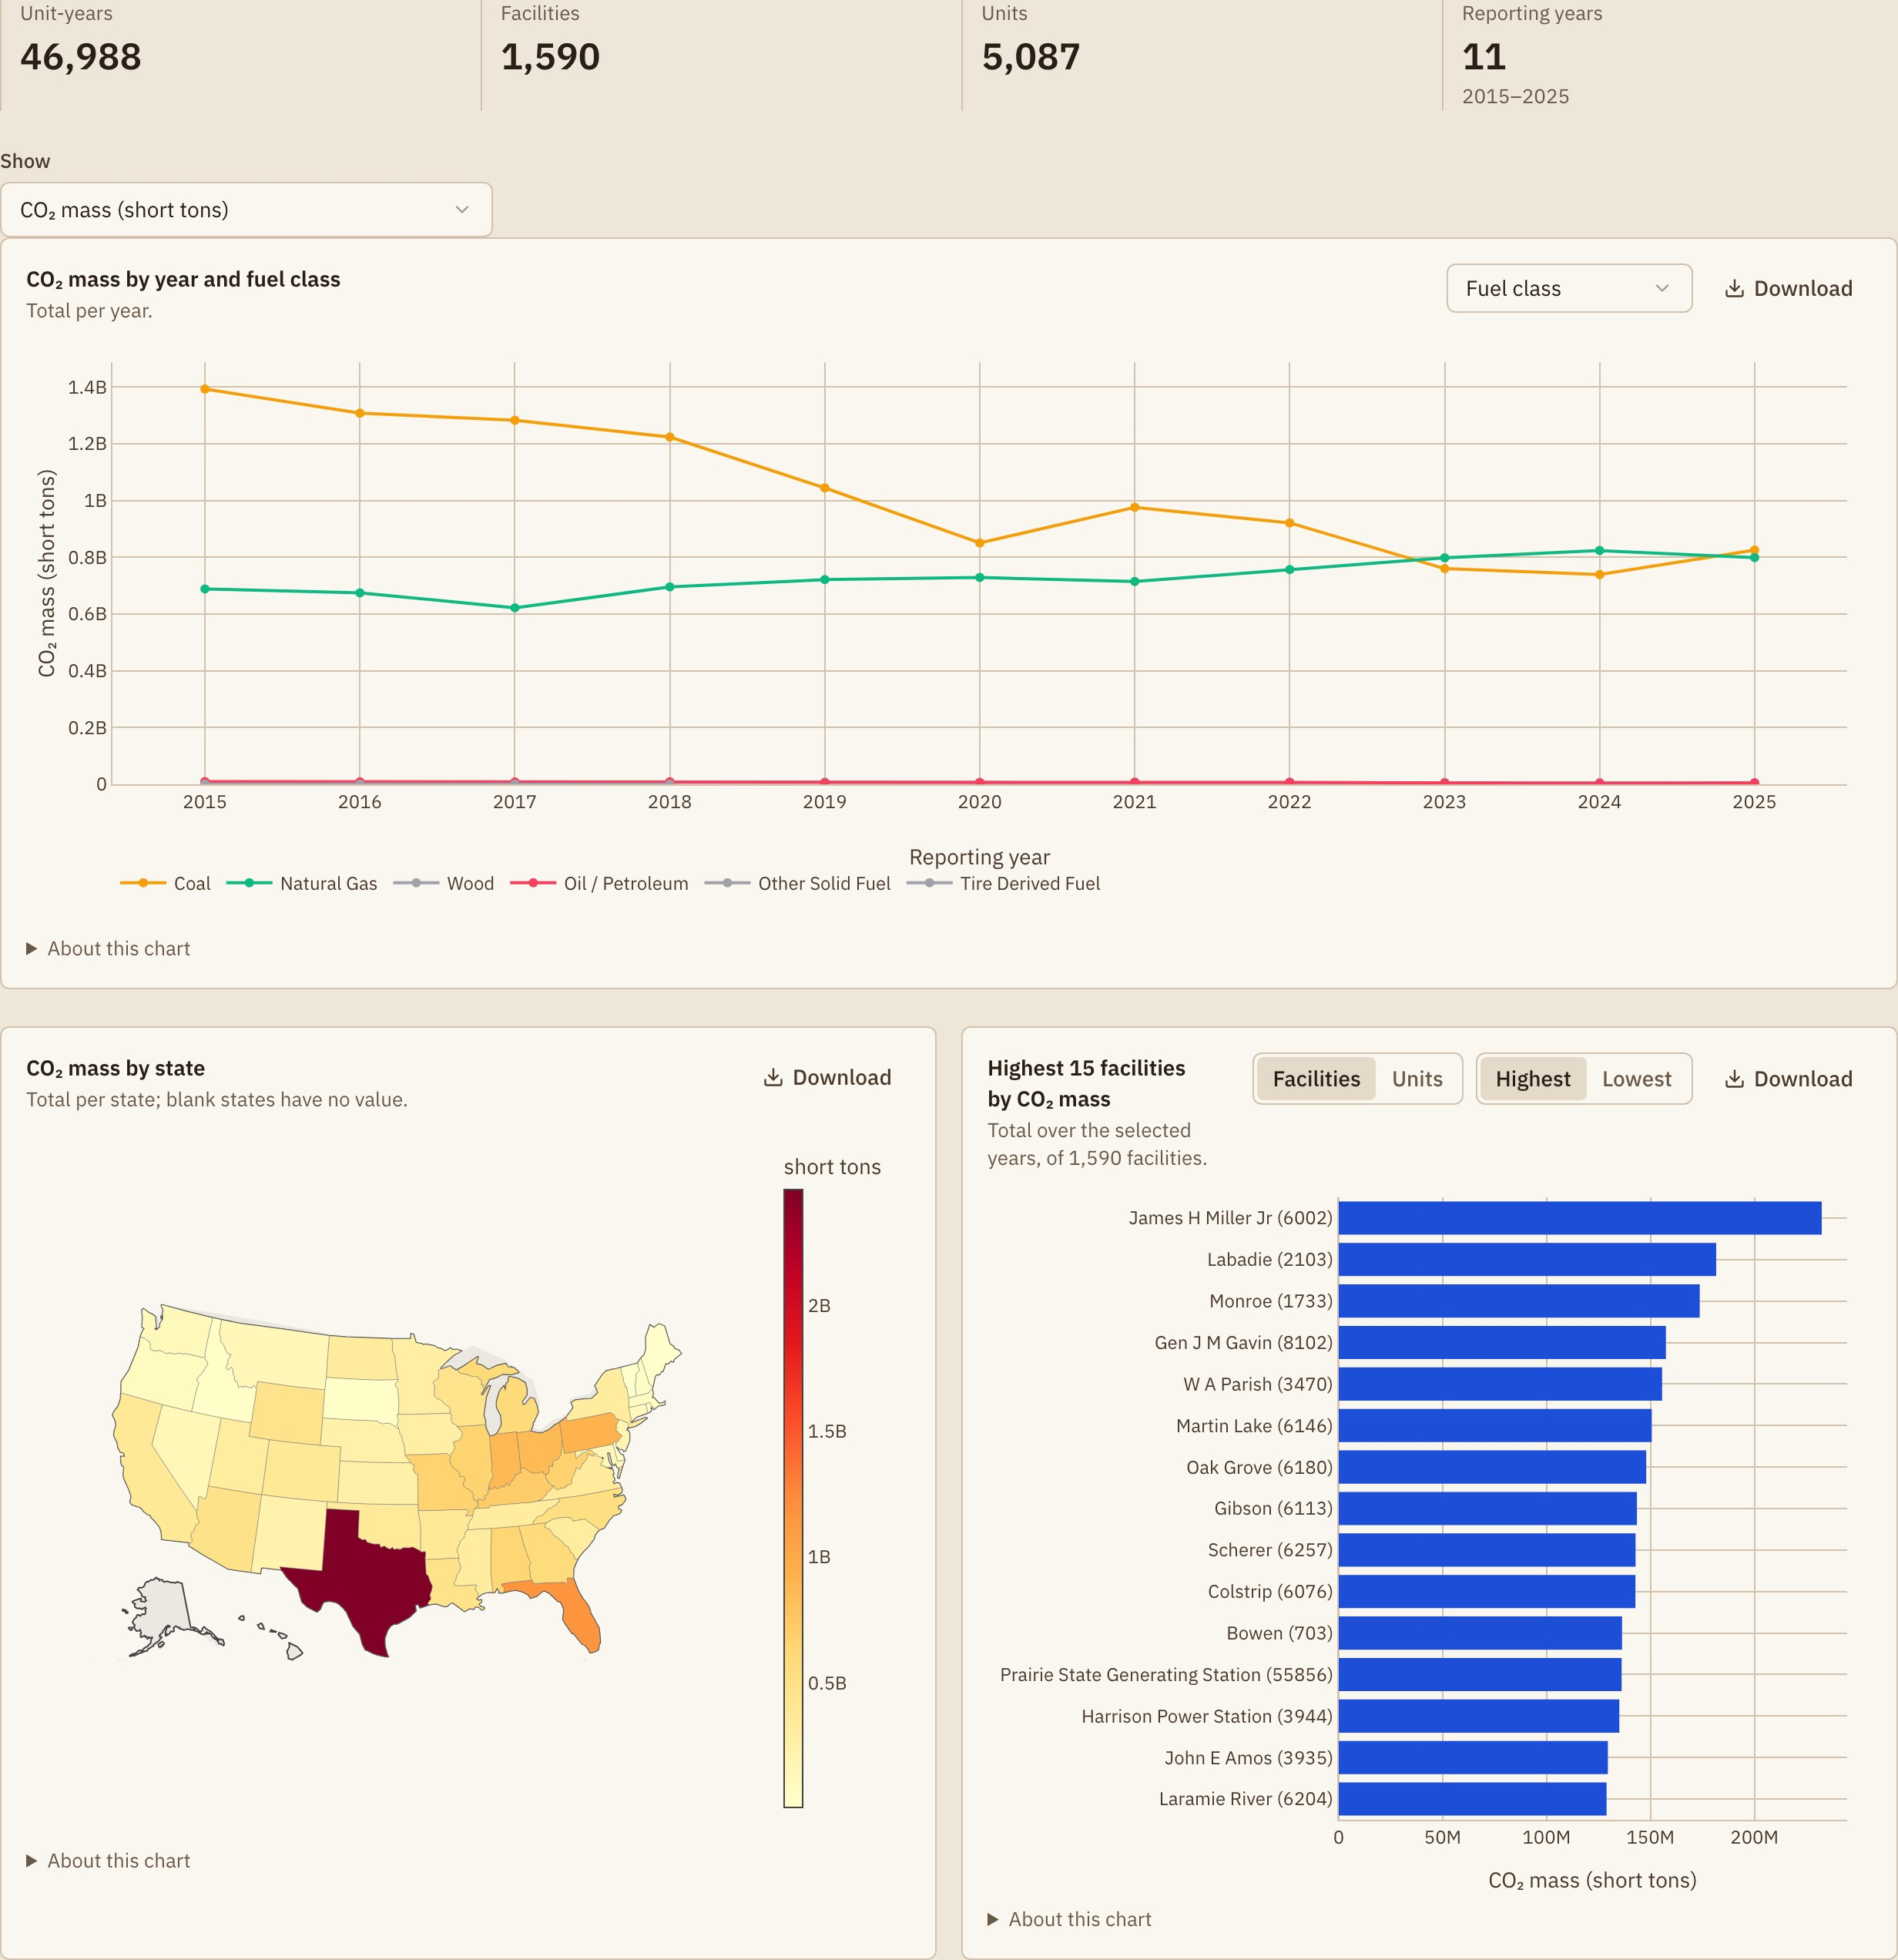
\includegraphics[width=\linewidth]{p2-overview.jpg}
  \caption{Overview tab for 2015--2025 (45{,}441 unit-years): filter chips, the reading, the
  \COtwo{} trend by fuel class, \COtwo{} by state, and the fifteen largest facilities.}
  \label{fig:overview}
\end{figure}

\subsection{Derived indicators}

Twenty-nine variables are available: seven measured values, six derived rates, eight
year-over-year changes, and eight TRACI indicators (Table~\ref{tab:variables}). Derived and TRACI
values are computed from the stored records each time an analysis runs, so they always match
the current data. Section~\ref{sec:methods} gives the definitions and the missing-value rules.

\subsection{Descriptive statistics}

The Distribution tab (Figure~\ref{fig:distribution}) describes one variable over the selection:
count, missing count, minimum, maximum, mean, median, standard deviation, first and third
quartiles, interquartile range (IQR), and the 5th, 10th, 90th, and 95th percentiles, plus the
variable's total, mean, or pooled rate over the whole selection. Six headline values come
first, then a histogram or box plot, then one sortable table with a row for the whole selection
and, with a grouping field, a row per group. It also lists \emph{unusual
observations}: unit-years beyond Tukey's far-out fences, $Q_1 - 3\,\text{IQR}$ and
$Q_3 + 3\,\text{IQR}$, with the count on each side and the ten most extreme. The four example
questions of the specification (average \COtwo{} by state, median \NOx{} intensity by fuel,
total \SOtwo{} by year, and average heat rate by unit type) are one-click examples.

\begin{figure}[!htbp]
  \centering
  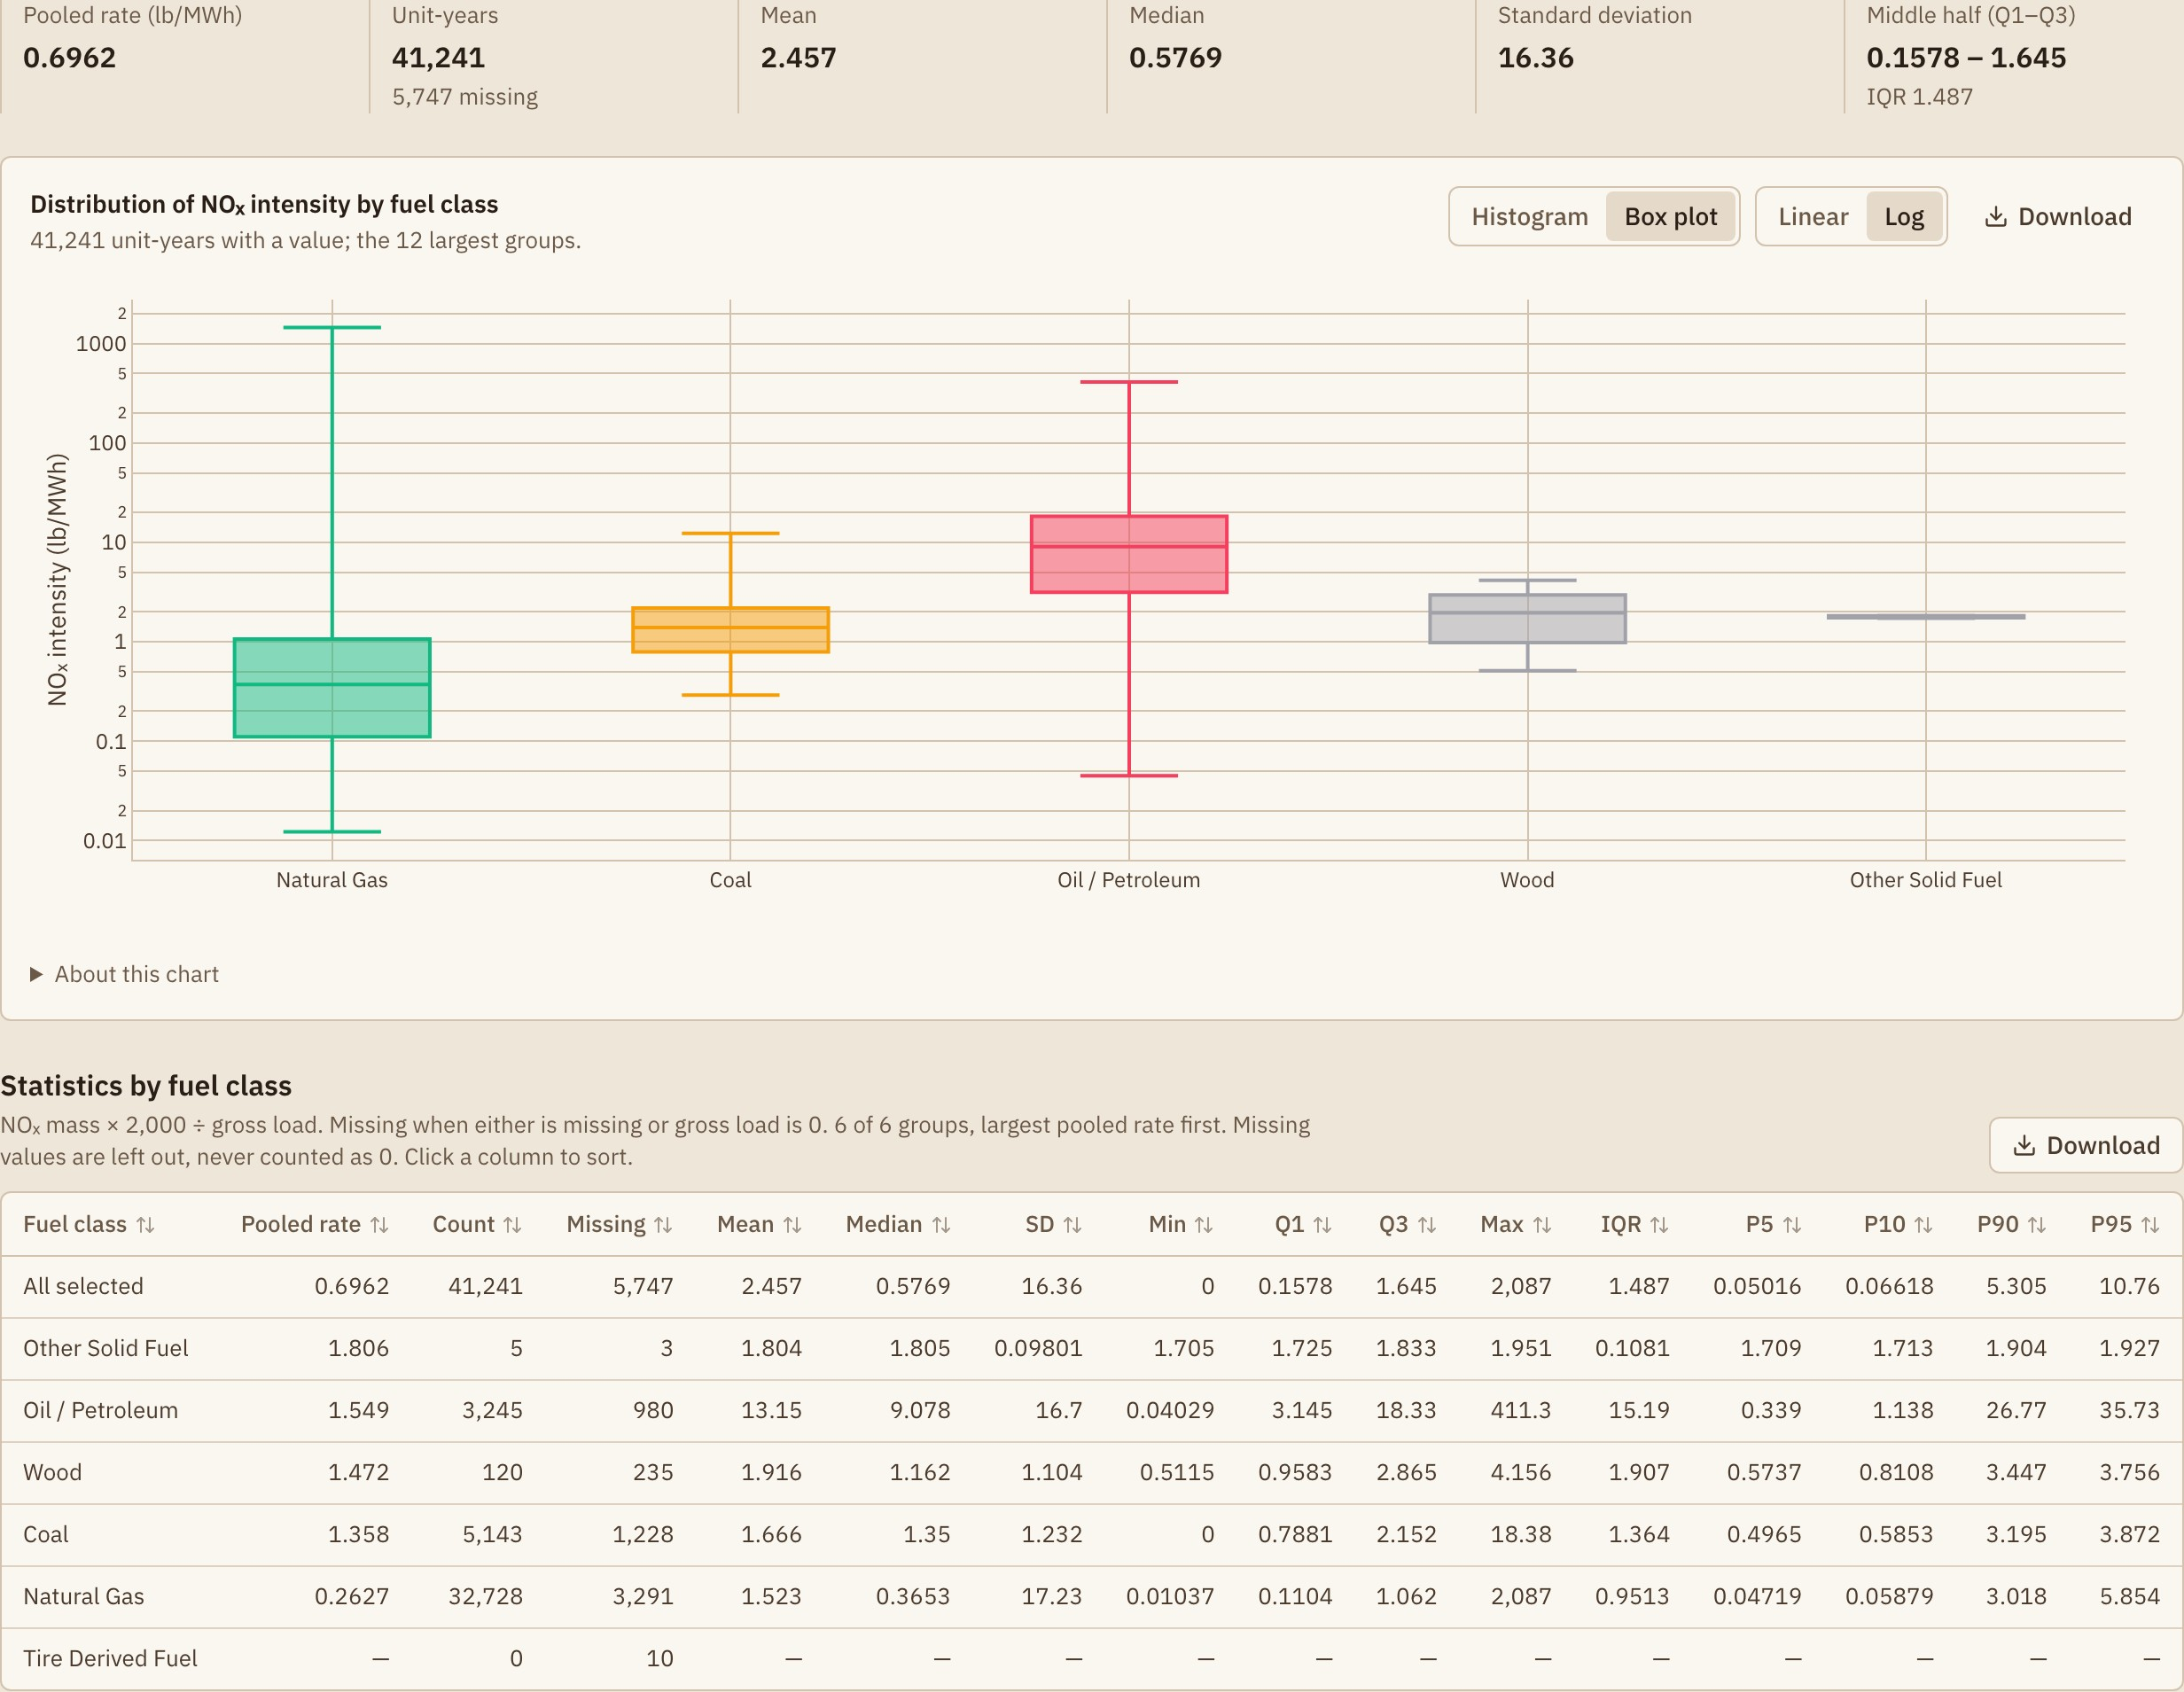
\includegraphics[width=\linewidth]{p2-distribution.jpg}
  \caption{Distribution tab: \NOx{} intensity over 2015--2025, overall and by fuel class (box
  plot on a log scale).}
  \label{fig:distribution}
\end{figure}

\subsection{Interactive visualization}

Seven chart types are drawn over the same selection, each on the tab whose question it answers:
on Overview, a trend of any variable per year with one line per group, a state choropleth, and
the top or bottom fifteen facilities or units; on Distribution, histograms and box plots,
optionally on a log scale and split by group; on Relationships, scatter plots of any two
variables, colored by group, and Pearson and Spearman correlation heat maps of eleven variables side by side;
and on Compare groups, bars for every group. Lines, bars, histograms, box plots, and scatter
plots are drawn with Recharts~\cite{recharts}; the state map and the heat map with
D3~\cite{bostock2011d3}, from U.S.\ state outlines bundled with the application. The Phase~1 Map
page still shows facility locations. Every chart has a descriptive title, a subtitle with the
unit, axis titles with units, a legend, tooltips with values and counts, and a \emph{Download}
button for its data, a PNG image, and metadata. Scatter plots zoom on both axes and line charts on
the horizontal axis by dragging over a region; on a phone, touch still scrolls the page. Log axes
use power-of-ten ticks. A chart whose query fails says so and offers to try again. Fuel classes
keep the colors they have on the Phase~1 map, and the models have colors of their own. For large
selections, distributions use an even sample of at most 20{,}000 values and scatter plots at
most 4{,}000 points, and the chart says so; statistics and correlations always use every value.
Figure~\ref{fig:charts} shows the two chart types not shown elsewhere in this report, a
histogram and a scatter plot; the trend, state map, and ranking are in
Figure~\ref{fig:overview}, the box plot in Figure~\ref{fig:box}, group bars in
Figure~\ref{fig:compare}, and the correlation heat map in Figure~\ref{fig:correlation}.

\begin{figure}[!htbp]
  \centering
  \begin{minipage}[t]{0.49\linewidth}
    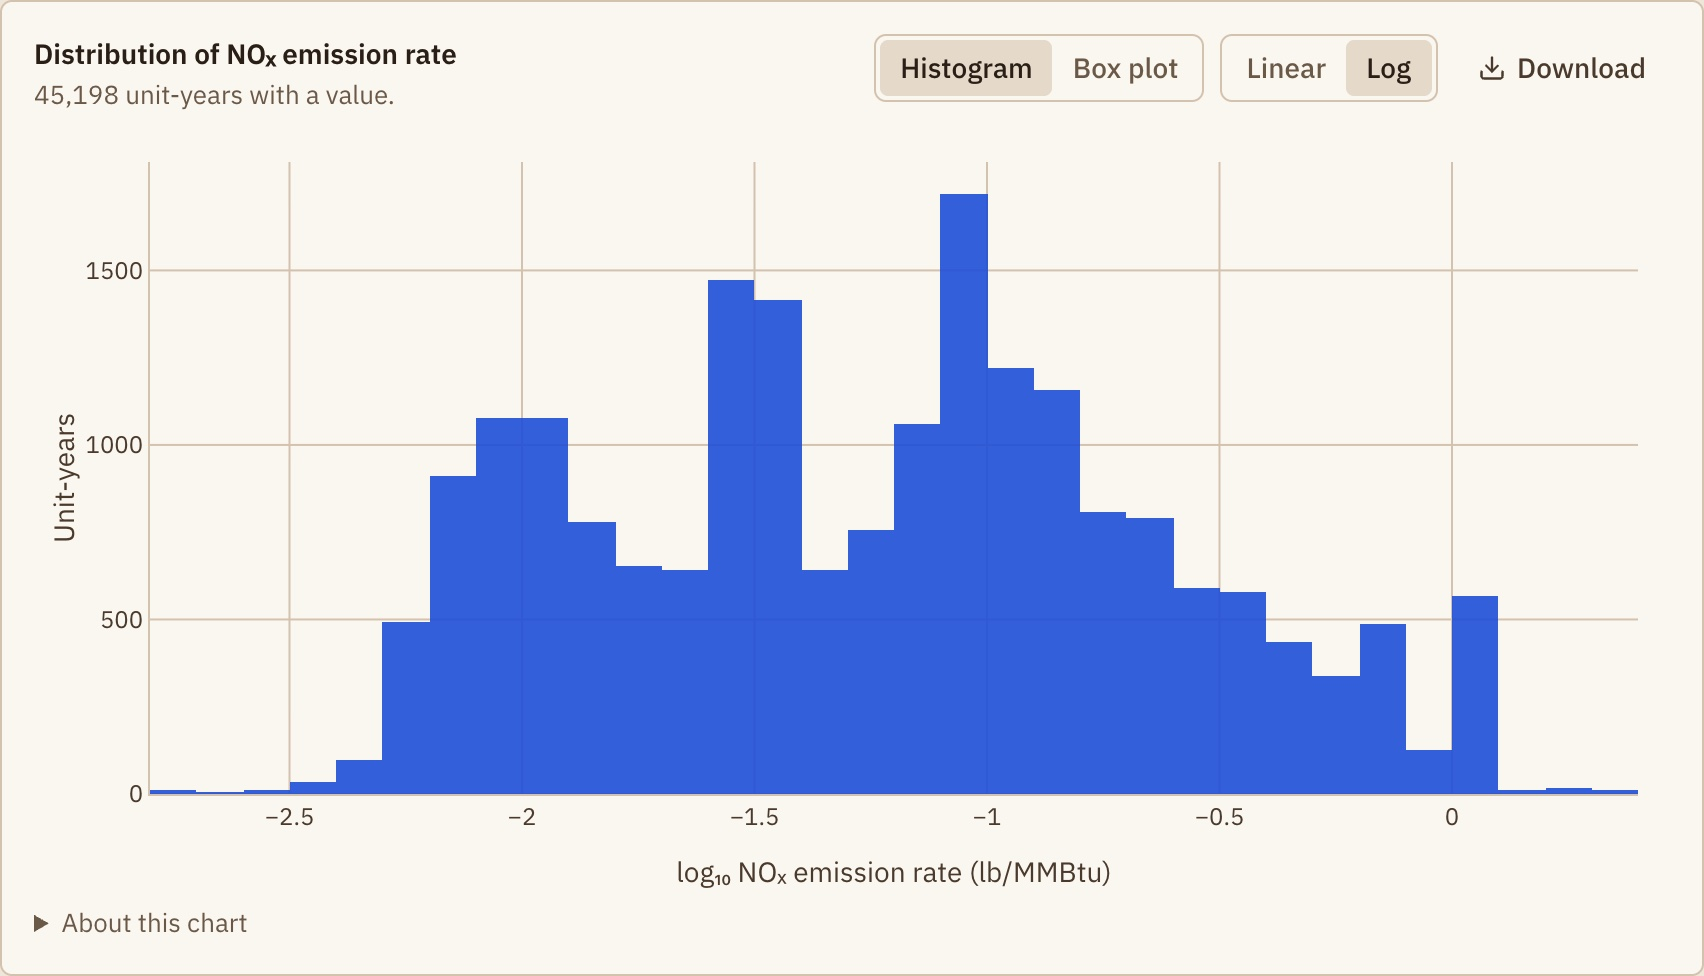
\includegraphics[width=\linewidth]{p2-histogram.jpg}
  \end{minipage}\hfill
  \begin{minipage}[t]{0.49\linewidth}
    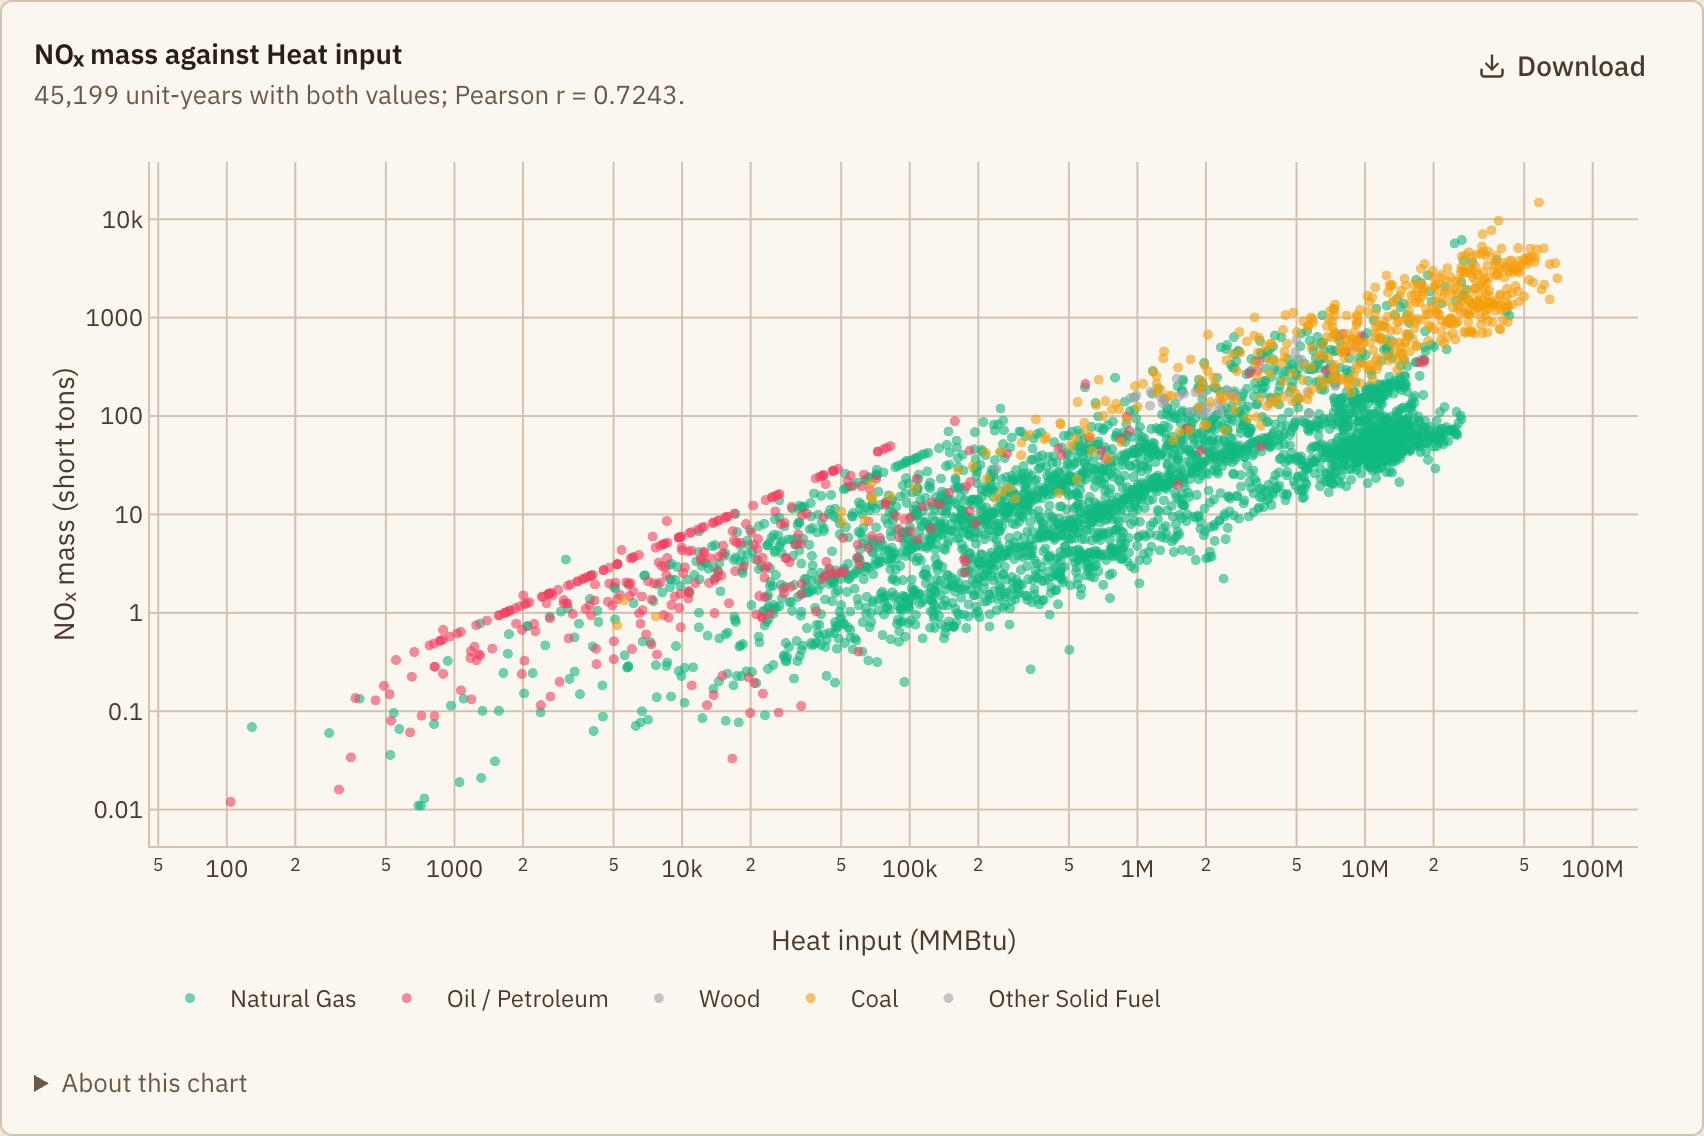
\includegraphics[width=\linewidth]{p2-scatter.jpg}
  \end{minipage}
  \caption{Left: histogram of the \NOx{} emission rate, 2015--2025, on a log scale (Distribution
  tab); the rate spans more than three orders of magnitude, with several peaks. Right: \NOx{}
  mass against heat input on log scales, colored by fuel class (Relationships tab). Since mass is
  rate times heat input, each fuel forms a band of slope about one, set higher or lower by its
  emission rate.}
  \label{fig:charts}
\end{figure}

\subsection{Comparative analysis}

The Compare groups tab first draws the variable for every group of the chosen field, then
compares two to eight of them: facilities or units (found with the search box), states, fuels,
unit types, \NOx{} or \SOtwo{} control classes (for example units with and without SCR), or reporting
years (for example 2015 against 2024). For each group it shows the pooled value of the variable,
its rank among the compared groups, its absolute and percentage difference from the first
group, the count, the mean with a 95\,\% confidence interval, the median, and the standard
deviation. It runs Welch's $t$-test and the Mann--Whitney $U$ test for two groups, and one-way
ANOVA and the Kruskal--Wallis test for any number, and states the result in plain language with
its caveats (Figure~\ref{fig:compare}). It opens on units with SCR against units with no \NOx{}
control. The Phase~1 comparison of two to four individual facilities or units is still
available from the Explore page, and its \emph{Analyze these} button opens the same selection
here, with every year and the tests. Likewise a facility's details link to Analyze and a unit's
details to Predict.

\subsection{Environmental and health impact indicators}

The TRACI impacts tab converts the selected emissions into four TRACI~2.2 impact categories (global
warming, acidification, particulate-matter human health, and smog formation), grouped by any
field. Each category is shown in its own equivalent unit, as a total or per MWh of gross load,
and categories are never added together. Each category's chart shows its own fifteen largest
groups. The full results table and the factors used are in collapsed sections; the factors are
listed with TRACI version,
substance, CAS number, and unit, and the formula of each category. It also states that the
results are potential impacts for comparison, not measured harm (Figure~\ref{fig:impacts}).

\subsection{Prediction}

The Models tab opens with a reading of the result: the best model's average error in tons and as
a share of the actual value, its gain over the baseline, and the persistence rule that beats it
(Section~\ref{sec:prediction}). Two charts follow: the test error (MAE) and the share of
variation explained ($R^2$) of the three registered models (baseline, Ridge regression, and
decision tree), each with 95\,\% bootstrap intervals (Figure~\ref{fig:models}). A collapsed table
compares all metrics on the validation and test years with the ablation. For the chosen model the
tab then plots predicted against actual \NOx{} for the test years, shows the tree's feature
importances or the Ridge coefficients in words and as bars, and charts the average signed error
by fuel class, which shows where the model is wrong and in which direction
(Figure~\ref{fig:errors}). \emph{All test predictions} downloads every test unit-year with each
model's prediction and error. A collapsed section gives the leakage rules and each model's
record: inputs, settings, the years it was fit and tuned on, saved file, software versions, and
training date.

\subsection{Sensitivity and scenario analysis}

The What-if tab asks one question as a sentence: \emph{What if} a baseline (one unit-year,
every unit at a plant, the units of a state, or of the whole country, chosen with the search box,
narrowed to a fuel if wanted) \emph{made} a change \emph{in} a year. The change is one of nine
named scenarios or any combination of power output, fuel burned, SCR, and primary fuel. Both
models, Ridge and the tree, are always shown side by side, each against its own baseline
prediction. The first chart draws one arrow per model from the prediction as reported to the
prediction after the change, next to the \NOx{} actually reported (Figure~\ref{fig:whatif}); a
group adds the units whose prediction changes most, and a single unit the tree's path in words.
The reading gives each model's change in tons and percent, whether it exceeds the model's typical
error, its share of the state's or nation's \NOx{}, and that the TRACI impacts of \NOx{} (smog,
acidification, particulate) change by the same share, since each is \NOx{} times a fixed factor.
A collapsed note lists every input the change sets, with its new and baseline value.

The scenario analysis compares the baseline with the nine named changes on the same units
(Figure~\ref{fig:scenarios}): add or remove SCR, run 10\,\% more or less (load and fuel together),
gross load $+10\,\%$ with heat input as reported, 5\,\% less fuel for the same power, a combined
high-efficiency case (5\,\% less fuel plus SCR), and a switch to gas or to coal. The subtitle
gives each model's baseline prediction in tons, each model's bar is labeled with its percentage
change from that baseline, the tooltip gives the baseline and scenario predictions with the
absolute and percentage change, and a reading names the change that cuts \NOx{} most, the one
that raises it most, and the rank of the user's question. A change that takes any unit outside
the training data is marked with a warning and the number of such units, and the CSV has the
baseline, prediction, absolute and percentage change, and that count for every scenario and
model.

The sensitivity analysis below varies one input and holds all others as reported. The user
chooses the input, a minimum, a maximum, and a step, as a percentage of the baseline value or,
for one unit, in the input's own unit (Figure~\ref{fig:sensitivity}). The curve marks the
baseline with a dot and dashed reference lines at the baseline input and at each model's baseline
prediction, and shades values outside the training data; the tooltip gives each input value
with its prediction and its absolute and percentage change and says when it is out of range, and
the exported CSV has the same columns. For a group, every unit's input is changed by the same
percentage and the totals are drawn, shaded wherever some unit's value leaves the training
range, with the number of such units in the reading and the CSV. The varied input can also be a category (primary fuel, unit type, or a \NOx{} control):
each model's prediction is then drawn as bars, one per value seen in training, with the unit's
own value marked (Figure~\ref{fig:category}).

\subsection{Saving and exporting results}
\label{sec:exports}

Every chart and the statistics, impact, and model-comparison tables have a \emph{Download}
button. Each downloads a ZIP file with the data as CSV, the chart as a PNG image (SVG, HTML, and
canvas charts alike), and a \code{metadata.json} file. The comparison, sensitivity, scenario, and
predicted-against-actual results are exported through their charts; the sensitivity CSV has the
absolute and percentage change and an out-of-range flag for every point, and \emph{All test
predictions} exports every one of the
7{,}755 test unit-years, not the chart's sample. The metadata records the export time and page URL; the
software version and Git commit; a snapshot of the database (unit-years, datasets, and time of
the last import), which serves as the dataset identifier; the filters and tab choices; the
definition, unit, and aggregation of each variable shown; the TRACI factors for impact results;
and, on the Predict page, the model's inputs, settings, fit and tuning years, metrics, saved file,
software versions, and the baseline unit-year. The full analytical dataset is exported by the
server (\code{/api/export?type=analysis}) in the same format, with the filters in place of the
URL. Section~\ref{sec:feat-export} shows an example.

\subsection{Readings, definitions, and input checks}
\label{sec:readings}

Results are interpreted, not only displayed, and inputs are validated. Three mechanisms serve
this.

\paragraph{Readings.} Each tab opens with a short block of sentences generated from the same
numbers as its charts (\code{src/lib/takeaways.ts}): a trend reads as a rise or fall between the
first and last year (``The yearly total of \COtwo{} mass fell 22\,\% from 2015 to 2025''); a
distribution as its middle half, its median, and whether the mean is pulled up by a few large
values; a correlation as a strength in words; a comparison as a difference with both tests and
their caveats; a model result as its error relative to the actual value and to the baseline; and
a scenario set as the largest change and the largest disagreement between models. Each function
returns nothing when there is nothing worth saying, and twelve unit tests cover them.

\paragraph{Definitions.} A glossary of 38 terms (\code{src/lib/glossary.ts}) marks the first
use of each term in a reading, subtitle, or note and in table headers, and shows its definition on
hover. Every variable's definition, unit, and missing-value rule is one click away.

\paragraph{Inputs.} Inputs the application cannot use are corrected and reported, never silently
dropped. On Analyze, an empty selection offers \emph{Clear filters}, a backwards year range offers
\emph{Swap years}, and \emph{Download all} is disabled when there is nothing to export; an unknown
variable sent to the server is answered with HTTP~400. On What-if, a minimum above the maximum is
read low to high, a step that is zero, negative, or empty becomes a twentieth of the range, a
range of more than 200 points is drawn with a wider step, negative values of a physical input are
dropped and counted (a range down to $-150\,\%$ of the baseline would otherwise ask for a negative
heat input), a scenario never sets an input below zero, and a message under the inputs says what
was drawn instead. A facility or unit ID that does not exist returns an empty result rather than
an error page.

\subsection{Requirement traceability}

Table~\ref{tab:trace} maps each requirement of the Phase~2 specification to the function that
meets it.

{\small
\begin{longtable}{@{}R{0.3\linewidth}R{0.5\linewidth}R{0.13\linewidth}@{}}
\caption{Phase~2 requirements and where they are met.}\label{tab:trace}\\
\toprule
\textbf{Specification} & \textbf{epaData} & \textbf{Status}\\
\midrule\endfirsthead
\toprule
\textbf{Specification} & \textbf{epaData} & \textbf{Status}\\
\midrule\endhead
\S1 Trends, relationships, unusual observations & Trend and correlation charts; Tukey far-out fences on the Distribution tab & Met\\
\S3 CAMPD multi-year data & 2015--2025 API years (and older uploads) in \code{annual\_records} & Met\\
\S3 TRACI version, pollutant, category, factor, unit stored & \code{traci\_factors} table & Met\\
\S4.1 Filters: years, state, facility, unit, fuel, unit type, controls, program, minimum operating time or load & Explore filter bar on Analyze & Met\\
\S4.1 Record, facility, unit, year counts; missing values; variables & Overview tab & Met\\
\S4.1 Reproducible through URL or saved configuration & URL parameters; filters in exported metadata & Met (URL)\\
\S4.2 Count, missing, min, max, mean, median, SD, quartiles, IQR, percentiles; grouped & Distribution tab & Met\\
\S4.3 \COtwo{}, \SOtwo{}, \NOx{} intensity; heat rate; year-over-year change; utilization & Derived variables; capacity factor & Met\\
\S4.3 Division by zero and missing values stay missing & Variable rules; unit tests & Met\\
\S4.4 Line, bar, histogram, box, scatter, correlation heat map, rankings & Overview, Distribution, Relationships, and Compare groups tabs & Met\\
\S4.4 State or facility-location maps & State choropleth; Phase~1 Map page & Met\\
\S4.4 Titles, units, legends, tooltips, filters, image and data download & Shared \code{Chart} component & Met\\
\S4.5 Facilities, units, states, fuels, unit types, with and without control, periods & Compare groups tab; Phase~1 compare dialog & Met\\
\S4.5 Statistics, differences, rankings, charts, normalized indicators, tests, plain language & Compare groups tab & Met\\
\S4.6 Short tons to kg; exact pollutant match; sum within category; per MWh; factors recorded & TRACI impacts tab; \code{impactVariables} & Met\\
\S5.1 One prediction target & Annual \NOx{} mass per unit-year & Met\\
\S5.2 Candidate features; no target leakage & Section~\ref{sec:prediction}; ablation & Met\\
\S5.3 Baseline and at least two models & Median baseline, Ridge, decision tree; persistence as a reference (Q4) & Met\\
\S5.4 Chronological split; MAE, RMSE, $R^2$, MAPE & 2016--21 / 2022--23 / 2024--25; 95\,\% bootstrap intervals on test metrics & Met\\
\S6.2 Model, baseline unit, input, minimum, maximum, step; value, prediction, changes, curve & What-if tab; both models shown side by side rather than picked (Table~\ref{tab:changes}) & Met\\
\S6.3 Baseline, load $+10\,\%$, heat input $-5\,\%$, fuel or control change, combined high efficiency; range warnings & Nine named changes on the What-if tab, each flagged when it leaves the training range & Met\\
\S6.4 Curve, baseline point and input and prediction reference lines, scenario bars, labels, out-of-range shading & What-if tab & Met\\
\S6.4 Same units; image or data export & Shared \code{Chart} component & Met\\
\S6.4 Response of impact indicators & The reading states the change in \NOx{}'s TRACI impacts, which move by the same share as predicted \NOx{} & Met\\
\S7 Export filtered dataset & \code{/api/export?type=analysis} & Met\\
\S7 Export statistics and comparison results & Statistics table; comparison chart & Met\\
\S7 Export model evaluation and predictions & Model-comparison table; predicted-against-actual chart; every test prediction & Met\\
\S7 Export sensitivity and scenario results & Sensitivity and scenario charts & Met\\
\S7 Export chart images or data & PNG (including HTML and canvas charts) and CSV in every chart's ZIP & Met\\
\S7 Metadata for reproducibility & \code{metadata.json} in every ZIP; a unit test checks each of the six items & Met\\
\S8 Steps 5 and 10: pandas analysis; Flask pages or JSON & Statistics in TypeScript, checked against NumPy and SciPy; tRPC procedures (Section~\ref{sec:design}) & Changed\\
\S8.1 Flask, Jinja2, SQLAlchemy, pandas, scikit-learn, joblib, pytest & Next.js, React, Drizzle; pandas, scikit-learn, joblib, and pytest offline & Changed\\
\S12.3 Instructions, migrations, environment template, tests, fixtures, no keys & README, migrations 0009--0010, \code{.env.example}, 116 + 10 tests, 120~KB fixture & Met\\
\bottomrule
\end{longtable}}

\subsection{Specified functions not completed or changed}
\label{sec:changes}

Every function in the Phase~2 specification was delivered (Table~\ref{tab:trace}).
Table~\ref{tab:changes} lists where the delivered system departs from the specification, and
why.

{\small
\begin{longtable}{@{}R{0.26\linewidth}R{0.27\linewidth}R{0.41\linewidth}@{}}
\caption{Departures from the specification.}\label{tab:changes}\\
\toprule
\textbf{Specified} & \textbf{Delivered} & \textbf{Reason}\\
\midrule\endfirsthead
\toprule
\textbf{Specified} & \textbf{Delivered} & \textbf{Reason}\\
\midrule\endhead
\S8.1, rubric: Phase~2 in the existing Flask application (Jinja2, Bootstrap) & Phase~2 in the existing Next.js application (React, tRPC, Drizzle) & The Phase~1 application is built on Next.js; the specification allows React for dashboards with extensive client-side state (Section~\ref{sec:discussion}).\\
\S8, steps 5 and 10: analysis with pandas & Statistics in TypeScript; pandas for training & One query per selection and no Python process per request; every statistic is checked against NumPy and SciPy.\\
\S8.1: Plotly.js for interactive charts & Recharts and D3 & Plotly charts did not match the interface and its theme; zoom and image export were rebuilt (Section~\ref{sec:discussion}).\\
\S8.1: models stored with joblib, metadata in the database & joblib files kept; each model also stored as JSON with its metadata & The browser replays the JSON, so What-if needs no Python server (Section~\ref{sec:design}).\\
\S5.2: state as a candidate feature & Not used & State is sparse within many fuel and unit-type combinations.\\
\S6.2: the user selects a trained model for sensitivity & What-if always shows Ridge and the tree side by side & Their disagreement is the main finding of Q4, and a single model would hide it; the Models tab still picks one model for its detail charts.\\
\bottomrule
\end{longtable}}

% ------------------------------------------------------------------------
\section{System design}
\label{sec:design}

\subsection{Architecture}

Phase~2 keeps the Phase~1 stack: Next.js~16~\cite{nextjs} with React~19~\cite{react}, tRPC
procedures for typed calls from the browser, Drizzle ORM, and SQLite~\cite{gaffney2022sqlite}.
The specification recommends Flask, with pandas and
scikit-learn for the analysis. We extended the Phase~1 application instead of porting it to Flask: a port
would have spent the phase re-implementing retrieval, upload, validation, and search rather than
building the analysis, and the specification allows React for dashboards with extensive
client-side state, which the Analyze and What-if pages are. Python still does what the
specification assigns to it, training and evaluating the models with pandas and scikit-learn.
For the analysis we chose a hybrid (Figure~\ref{fig:architecture}).
Statistics, indicators, and TRACI impacts are computed in TypeScript on the server, next to the
database. Models are trained offline in Python with pandas and
scikit-learn~\cite{pedregosa2011sklearn}, and each trained model is stored in the database with
its preprocessing and parameters as JSON, which a small TypeScript module replays exactly.
Predictions, sensitivity curves, and scenarios therefore need no Python process at request time
and also run on the hosted build, where Python is not available.

\begin{figure}[!htbp]
  \centering
  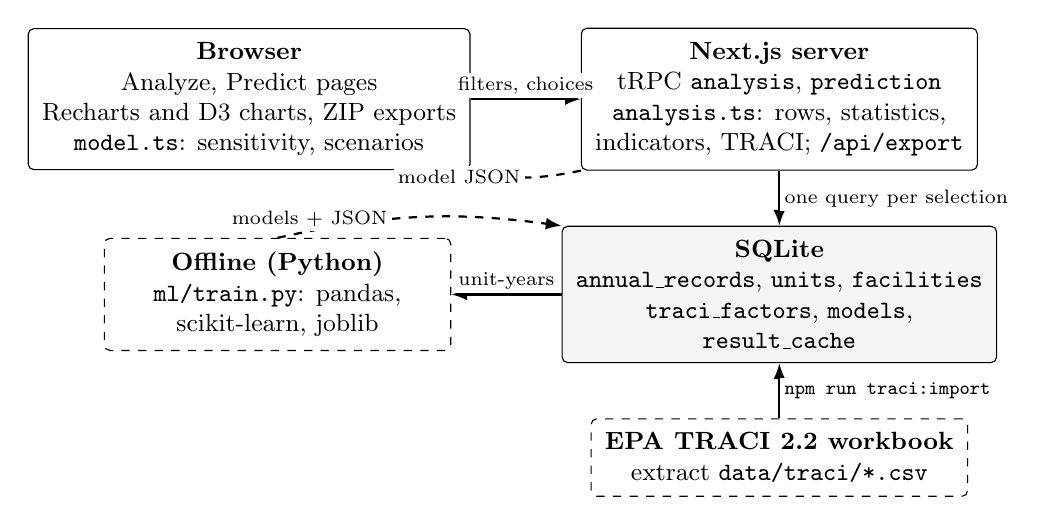
\begin{tikzpicture}[node distance=7mm and 9mm]
    \node[box, minimum width=4.4cm] (pages) {\textbf{Browser}\\Analyze, Predict pages\\Recharts and D3 charts, ZIP exports\\\code{model.ts}: sensitivity, scenarios};
    \node[box, right=14mm of pages, minimum width=4.6cm] (server) {\textbf{Next.js server}\\tRPC \code{analysis}, \code{prediction}\\\code{analysis.ts}: rows, statistics,\\indicators, TRACI; \code{/api/export}};
    \node[store, below=of server, minimum width=4.6cm] (db) {\textbf{SQLite}\\\code{annual\_records}, \code{units}, \code{facilities}\\\code{traci\_factors}, \code{models},\\\code{result\_cache}};
    \node[ext, left=14mm of db, minimum width=4.4cm] (train) {\textbf{Offline (Python)}\\\code{ml/train.py}: pandas,\\scikit-learn, joblib};
    \node[ext, below=of db, minimum width=4.6cm] (traci) {\textbf{EPA TRACI 2.2 workbook}\\extract \code{data/traci/*.csv}};
    \draw[flow] (pages) -- node[lbl, above] {filters, choices} (server);
    \draw[flow] (server) -- node[lbl, right] {one query per selection} (db);
    \draw[flow] (db) -- node[lbl, above] {unit-years} (train);
    \draw[lflow] (train.north) to[bend left=10] node[lbl, left, pos=0.4] {models + JSON} (db.north west);
    \draw[flow] (traci) -- node[lbl, right] {\code{npm run traci:import}} (db);
    \draw[lflow] (server.south west) to[bend left=12] node[lbl, left, pos=0.5] {model JSON} (pages.south east);
  \end{tikzpicture}
  \caption{Phase~2 architecture. Solid arrows run on every request or import; dashed arrows
  carry the trained models from the offline pipeline to the browser.}
  \label{fig:architecture}
\end{figure}

\subsection{Life cycle of an analysis}

When a tab needs a result, the browser calls a tRPC procedure with the filters and the tab's
choices. The server turns the filters into the same SQL conditions the Explore page uses (one
shared function, \code{unitYearConditions}) and selects the matching unit-years, joined with
their unit, their facility, and the same unit's previous year, which the year-over-year
variables need. The rows are cached for five minutes, keyed by the filters and the time of the
latest import, because one page usually asks for several views of the same selection. The
variables are evaluated in memory and only the result (a table, chart points, or a matrix) is
returned. Slower results are first looked up in \code{result\_cache}, so a view opened before
on the same data is read rather than recomputed. Section~\ref{sec:perf} gives the measured times.

\subsection{Database additions}

Phase~2 adds three tables. Migration 0009 adds two. \code{traci\_factors} holds one row per TRACI version,
pollutant, medium, and impact category, with the TRACI substance name, CAS number, factor, unit,
and the workbook column it was read from; a unique index prevents duplicates. It is loaded from
a six-row extract of the EPA workbook (\code{data/traci/traci\_2\_2\_air.csv}), whose source,
download date, and checksum are recorded next to it. \code{models} holds one row per trained
model: name and kind, target, inputs, tuned settings, training, validation, and test years,
metrics, the JSON artifact used for prediction, the path of the saved scikit-learn object, and
the software versions and Git commit that produced it. The committed database contains six
factors and three models. Migration 0010 adds \code{result\_cache}, which stores the results of
the slower analyses (summary, statistics, aggregates, distributions, scatter plots,
correlations, and comparisons) keyed by procedure and input, with the version of the data they
were computed from: the time of the latest import, a hash of the TRACI factors, and a version of
the analysis code. An import or a factor change makes old results unreachable at once, and
\code{npm run db:precompute} recomputes the stored ones; the committed database ships 90.
Column-level documentation is in \code{DATABASE\_BREAKDOWN.md}.

\subsection{Data flow and reproducibility}

A Phase~2 result can be traced back through five steps. CAMPD records enter the database
through retrieval or upload, as in Phase~1, and each record keeps the dataset that last wrote
it. \code{npm run traci:import} loads the factor extract, whose checksum ties it to the EPA
workbook. \code{npm run ml:train} reads the unit-years, trains and evaluates the models, and
writes them with their metrics and software versions to the \code{models} table, together with
the fixture used by the parity test. An analysis evaluates the variables for the selected
unit-years. An export writes the result with the filters, variable definitions, factors or model
record, the Git commit, and the database snapshot. Opening the recorded URL on a database with
the same snapshot reproduces the same numbers.

% ------------------------------------------------------------------------
\section{Technical details}
\label{sec:technical}

\subsection{Languages}

TypeScript implements the interface, the server, the statistics, the TRACI calculation, and
model inference. Python implements the offline training pipeline (\code{ml/train.py}) and, as in
Phase~1, the upload parser. SQL is mostly generated by Drizzle; the selection of unit-years with
their previous year is a self-join written as a Drizzle query.

\subsection{Frameworks and libraries}

Table~\ref{tab:stack} lists what Phase~2 adds to the Phase~1 stack. The committed models were
trained with Python~3.15 and the versions in the table. The minimum versions in
\code{requirements.txt} allow the Python~3.9 documented in the README. On Python~3.9.25 with the
newest versions it installs (pandas 2.3, NumPy 2.0, scikit-learn 1.6), the pipeline tests pass
and retraining gives the same Ridge and baseline models; the tree's test MAE differs by
0.0001~t, and no reported value changes at the precision shown. NumPy 2.0 on macOS prints
spurious overflow warnings from the bootstrap's matrix products; on the same inputs the bootstrap
gives identical intervals on both versions.

\begin{table}[H]
\centering\small
\caption{Libraries added in Phase~2.}
\label{tab:stack}
\begin{tabularx}{\linewidth}{@{}>{\raggedright\arraybackslash}p{0.3\linewidth}L@{}}
\toprule
\textbf{Component} & \textbf{Role in epaData}\\
\midrule
Recharts 3.10~\cite{recharts} & Line, bar, histogram, box-plot, and scatter charts: tooltips, legends, drag-to-zoom.\\
D3 7.9~\cite{bostock2011d3}, topojson-client & State choropleth and correlation heat map; color scales; U.S.\ outlines from us-atlas, bundled in \code{public/geo/}.\\
fflate & Builds the ZIP exports in the browser and on the server.\\
pandas 3.1~\cite{mckinney2010pandas}, NumPy 2.5~\cite{harris2020numpy} & Feature extraction and preprocessing in \code{ml/train.py}.\\
scikit-learn 1.9.1~\cite{pedregosa2011sklearn} & Ridge regression, decision tree, metrics.\\
joblib & Saves the fitted scikit-learn objects (\code{ml/models/*.joblib}).\\
SciPy 1.18~\cite{virtanen2020scipy} & Reference values for the statistics tests.\\
pytest & Tests of the training pipeline (\code{ml/test\_pipeline.py}).\\
\bottomrule
\end{tabularx}
\end{table}

\subsection{External services}

\textbf{Vercel} hosts the application at \url{https://epadata.vercel.app}. The hosted build
is read-only (\code{READ\_ONLY=true}): Upload and Retrieve show a notice to run the application
locally, while Analyze and Predict work fully because they only read the committed database.
The state outlines for the choropleth are bundled with the application, so Analyze and Predict
need no outside service; only the Phase~1 flat map loads CARTO background tiles. Phase~2 adds no
API keys; \code{.env.example} is unchanged.

\subsection{Scripts and configuration}

Table~\ref{tab:scripts} lists the scripts added in Phase~2. The Phase~1 scripts are unchanged.

\begin{table}[H]
\centering\small
\caption{Scripts added in Phase~2.}
\label{tab:scripts}
\begin{tabularx}{\linewidth}{@{}>{\raggedright\arraybackslash}p{0.3\linewidth}L@{}}
\toprule
\textbf{Command} & \textbf{Purpose}\\
\midrule
\code{npm run traci:import} & Loads \code{data/traci/traci\_2\_2\_air.csv} into \code{traci\_factors}.\\
\code{npm run ml:train} & Trains, tunes, and evaluates the models; writes \code{ml/models/}, the \code{models} rows, and the parity fixture.\\
\code{npm run test:py} & Runs the pytest tests of the training pipeline.\\
\code{npm test} & Runs all 116 TypeScript tests, including the Phase~2 ones.\\
\code{npm run report} & Builds this report with Tectonic.\\
\bottomrule
\end{tabularx}
\end{table}

% ------------------------------------------------------------------------
\section{Methods}
\label{sec:methods}

\subsection{Variables and missing values}

Table~\ref{tab:variables} defines the derived variables. A value is \emph{missing} when CAMPD did
not report it, or when an input of a derived value is missing or its denominator is zero or
negative. Missing values are left out of statistics and counted separately. They are never
treated as zero, which would pull every mean and intensity down.

{\small
\begin{longtable}{@{}R{0.24\linewidth}R{0.16\linewidth}R{0.52\linewidth}@{}}
\caption{Derived variables (computed per unit-year).}\label{tab:variables}\\
\toprule
\textbf{Variable} & \textbf{Unit} & \textbf{Definition}\\
\midrule\endfirsthead
\toprule
\textbf{Variable} & \textbf{Unit} & \textbf{Definition}\\
\midrule\endhead
\COtwo{}, \SOtwo{}, \NOx{} intensity & lb/MWh & mass (short tons) $\times$ 2{,}000 $\div$ gross load\\
\NOx{} emission rate & lb/MMBtu & \NOx{} mass $\times$ 2{,}000 $\div$ heat input\\
Heat rate & MMBtu/MWh & heat input $\div$ gross load\\
Capacity factor & \% & gross load $\div$ (nameplate MW $\times$ hours in the year) $\times$ 100; 8{,}784 hours in leap years; values above 100\,\% are kept\\
Change (load, \COtwo{}, \SOtwo{}, \NOx{}) & MWh or tons & this year minus the same unit's previous year\\
Change (\%) & \% & (this year $-$ previous year) $\div$ previous year $\times$ 100\\
TRACI impact, category $c$ & kg eq & $\sum_i$ mass$_{i,\text{kg}}$ $\times$ CF$_{i,c}$ (Section~\ref{sec:traci})\\
TRACI impact per MWh & kg eq/MWh & impact $\div$ gross load\\
\bottomrule
\end{longtable}}

\paragraph{Combining groups.} Each variable has one rule for combining unit-years into a group
value. Masses, energy, changes in tons, and impacts are summed. Operating time and nameplate
capacity are averaged per unit-year. Rates are \emph{pooled}: the sum of the numerators divided
by the sum of the denominators, over the unit-years where the rate is defined. A state's
\COtwo{} intensity is therefore its total \COtwo{} divided by its total gross load, not the mean
of its units' intensities. The mean would give a peaking turbine that ran ten hours the same
weight as a baseload coal unit.

\subsection{Descriptive statistics and correlation}

Quantiles use linear interpolation between order statistics, $Q(p) = x_{(\lfloor h\rfloor)} +
(h - \lfloor h\rfloor)(x_{(\lfloor h\rfloor + 1)} - x_{(\lfloor h\rfloor)})$ with $h = (n-1)p$,
which is Hyndman and Fan's type~7~\cite{hyndman1996quantiles} and NumPy's default. The standard
deviation is the sample standard deviation ($n - 1$). Pearson's $r$ and Spearman's $\rho$
(Pearson's $r$ of average ranks) use the unit-years where both variables are reported.

\subsection{Comparisons and tests}

The 95\,\% confidence interval of a group mean is $\bar{x} \pm t_{0.975,\,n-1}\, s/\sqrt{n}$.
Two groups are compared with Welch's $t$-test~\cite{welch1947}, which does not assume equal
variances, and with the Mann--Whitney $U$ test~\cite{mann1947} (normal approximation with tie
correction), which asks whether one group tends to have larger values and is robust to the
heavy tails of emissions data. Three or more groups are compared with one-way ANOVA and the
Kruskal--Wallis test~\cite{kruskal1952}. The $t$, $F$, $\chi^2$, and normal distribution
functions are computed in TypeScript from the regularized incomplete beta and gamma functions
and checked against SciPy~\cite{virtanen2020scipy}.

Two assumptions limit these tests, and the page states both. First, the groups differ in more
than the attribute compared (size, age, fuel, hours run), so a difference is an association, not
an effect of that attribute. Second, the tests treat every unit-year as independent, but the
same unit appears in several years, so the $p$-values are smaller than they should be.

\subsection{TRACI impact assessment}
\label{sec:traci}

CAMPD supplies the inventory, the mass of each pollutant a unit emitted in a year. TRACI supplies
characterization factors~\cite{bare2011traci,epa2022traci22}: the potential contribution of one
kilogram of a substance emitted to air to an impact category. The two are joined by a fixed
mapping from CAMPD pollutant to TRACI substance, never by approximate name matching. CAMPD's
\COtwo{} maps to \emph{CARBON DIOXIDE} (CAS 124-38-9), \SOtwo{} to \emph{SULFUR DIOXIDE} (CAS
7446-09-5), and \NOx{} to \emph{NITROGEN OXIDES}, which has no CAS number in TRACI. TRACI also
lists \emph{NITROGEN DIOXIDE}, with a smog factor of 16.85~kg~O\textsubscript{3}~eq/kg against
24.79 for nitrogen oxides. CAMPD reports \NOx{}, so the nitrogen-oxides row is the right one.
Table~\ref{tab:factors} lists every non-empty air factor of the three substances in the TRACI~2.2
workbook.

\begin{table}[H]
  \centering\small
  \caption{TRACI~2.2 factors used (per kg emitted to air).}\label{tab:factors}
  \begin{tabular}{@{}llll@{}}
    \toprule
    \textbf{Category} & \textbf{\COtwo{}} & \textbf{\SOtwo{}} & \textbf{\NOx{}}\\
    \midrule
    Global warming (kg \COtwo{} eq) & 1 & --- & ---\\
    Acidification (kg \SOtwo{} eq) & --- & 1 & 0.7\\
    Human health, particulate (kg \PMtwofive{} eq) & --- & 0.061111 & 0.0072222\\
    Smog formation (kg O\textsubscript{3} eq) & --- & --- & 24.793590\\
    \bottomrule
  \end{tabular}
\end{table}

For each unit-year, CAMPD masses are converted from short tons to kilograms and multiplied by
their factors, summing only within a category:
\begin{align}
  \text{Mass}_{i,\text{kg}} &= \text{Mass}_{i,\text{short ton}} \times 907.18474,\\
  \text{Impact}_c &= \sum_i \text{Mass}_{i,\text{kg}} \times \text{CF}_{i,c},\\
  \text{Impact intensity}_c &= \text{Impact}_c \,/\, \text{Gross load}_{\text{MWh}}.
\end{align}
Categories keep their own units and are never added together. If a pollutant that contributes
to a category was not reported, that category is missing for the unit-year, while categories
that do not need the pollutant are still computed: a unit-year without \SOtwo{} has no
acidification result but does have a smog result. Group results are sums of unit-year results,
and group intensities are pooled as above.

\paragraph{Worked example.} In 2024 the four units of Ghent (facility 1356, Kentucky) reported
11{,}399{,}877.916 short tons of \COtwo{}, 9{,}157.169 tons of \SOtwo{}, 6{,}987.671 tons of
\NOx{}, and a gross load of 11{,}580{,}029.2~MWh. Acidification is $(9{,}157.169 \times 1 +
6{,}987.671 \times 0.7) \times 907.18474 = 14{,}048.539 \times 907.18474 = 12{,}744{,}620$~kg
\SOtwo{}~eq, or 1.1006~kg \SOtwo{}~eq per MWh. Global warming is $11{,}399{,}877.916 \times
907.18474 = 1.0342 \times 10^{10}$~kg \COtwo{}~eq; particulate human health is
553{,}447~kg~\PMtwofive{}~eq; smog formation is $1.5717 \times 10^{8}$~kg O\textsubscript{3}~eq.
The TRACI impacts tab, grouped by facility for 2024, shows the same values.

\subsection{Prediction}
\label{sec:prediction}

\paragraph{Target.} The models predict a unit's annual \NOx{} mass in short tons. We chose \NOx{}
over \COtwo{} because \COtwo{} is close to a fixed multiple of heat input for a given fuel, so a
\COtwo{} model would mostly learn that multiple. \NOx{} depends on combustion conditions and
controls, so the controls carry information, and every scenario in the specification (changed
load, changed heat input, changed control) affects the prediction.

\paragraph{Inputs.} Heat input, gross load, and operating time of the same year; nameplate
capacity; unit age (reporting year minus the year of commercial operation); the unit's \NOx{}
rate (lb/MMBtu) and operating time in the previous year; primary fuel and unit type; and five
\NOx{} control flags (SCR, SNCR, low-\NOx{} burners, water, steam, or ammonia injection, and
overfire air), read from the controls reported that year.

\paragraph{Leakage.} No input is the target or is computed from it: same-year \NOx{} mass,
\NOx{} rate, and \NOx{} intensity are excluded. The previous year's \NOx{} rate is allowed because
it is known before the year starts. Same-year heat input, gross load, and operating time are not
known in advance, but they are what the scenarios change, so they are kept. To show how much
accuracy they provide, every model is also fitted without them (the ablation column of
Table~\ref{tab:models}).

\paragraph{Split.} Unit-years from 2016 (the first year with a previous year) to 2025 with a
reported \NOx{} mass are split by year: 25{,}116 training unit-years (2016--2021), 7{,}970
validation unit-years (2022--2023), and 7{,}755 test unit-years (2024--2025). Settings are chosen
on the validation years; the chosen models are then refit on 2016--2023 and evaluated once on
2024--2025. A random split was not used because it would let a model learn a unit's 2024
emissions from its 2025 record.

\paragraph{Models.} The baseline predicts the median \NOx{} of training unit-years with the same
primary fuel and unit type, or the overall median for unseen combinations. Ridge
regression~\cite{hoerl1970ridge} is fitted to $\log(1 + \text{NO}_x)$, because \NOx{} spans six
orders of magnitude, with the penalty $\alpha$ chosen from $\{0.01, 0.1, 1, 10, 100\}$; its
predictions are transformed back and floored at zero. The decision tree~\cite{breiman1984cart}
is fitted to tons, with the maximum depth chosen from $\{4, 6, 8, 10, 12, 16, 20, 24\}$ or
unlimited and the minimum leaf size from $\{5, 20, 50\}$. Validation selected $\alpha = 10$ and a
maximum depth of 20 with at least 20 unit-years per leaf. An earlier grid stopped at depth 16 and
chose its top value, so it was extended. The extension changes nothing: with 20 unit-years per
leaf the tree stops growing at depth 18 by itself, so limits of 20, 24, and none give the same
tree, and its validation MAE differs from the depth-16 tree's by 0.001 tons.

\paragraph{Persistence reference.} A model can only be judged against a fair alternative. Besides
the required median baseline, \code{train.py} computes a \emph{persistence} reference: the unit's
previous-year \NOx{} rate times this year's heat input, divided by 2{,}000, or the median
baseline when either is missing (1.4\,\% of test unit-years). It uses only inputs the models
also see. In the ablation, where same-year heat input is unknown, it predicts last year's tons.
It is reported with the metrics (\code{ml/models/metrics.json}) but not registered as a model
or shown in the application.

\paragraph{Metrics.} Mean absolute error (MAE), root mean squared error (RMSE), coefficient of
determination ($R^2$), and mean absolute percentage error (MAPE). MAPE is computed only over
unit-years of at least one ton, because for peaking turbines that emit a fraction of a ton a
percentage error has no useful meaning. Each test metric has a 95\,\% percentile interval from
1{,}000 bootstrap samples. Because the test years hold up to two unit-years of each unit, which
are not independent, each sample draws units with replacement and keeps all of a drawn unit's
years (a cluster bootstrap). The same samples give an interval for the difference between a
model's MAE and the persistence reference's.

\paragraph{Sensitivity and scenarios.} A sensitivity curve changes one input of the baseline
unit-year at each step, holds every other input fixed, and records the prediction, its absolute
change, and its percentage change, $(\hat{y}_{\text{scenario}} - \hat{y}_{\text{baseline}}) /
\hat{y}_{\text{baseline}} \times 100$. An input is \emph{outside the training data} when it is
below the minimum or above the maximum of that input in the training years, or when its fuel or
unit type was not seen in training. The check is per input, so a combination of individually
ordinary values can still be unlike any training unit-year.

% ------------------------------------------------------------------------
\section{Results}
\label{sec:results}

All results use the reporting years 2015--2025 of the committed database unless stated
otherwise.

\subsection{Q1: emissions trends and the shift from coal to gas}

Total \COtwo{} from the selected units fell from 2{,}098 million short tons in 2015 to 1{,}635
million in 2025 (22\,\%), and the pooled \COtwo{} intensity fell from 1{,}557 to 1{,}279 lb/MWh
(18\,\%). Figure~\ref{fig:trend} shows where the decline came from. Coal units emitted 1{,}393
million tons in 2015 and 739 million in 2024, while gas units rose from 688 to 824 million. The
two lines crossed twice: in 2023 gas units emitted more \COtwo{} than coal units for the first
time in the data, and in 2025 coal was ahead again (825 against 799 million). The intensity of
each fuel changed little: coal units averaged 2{,}041 lb/MWh in 2015 and 2{,}036 in 2025, gas
units 1{,}051 and 926. The sector's falling intensity is therefore mainly a change in the
generation mix, not cleaner coal plants.

\begin{figure}[!htbp]
  \centering
  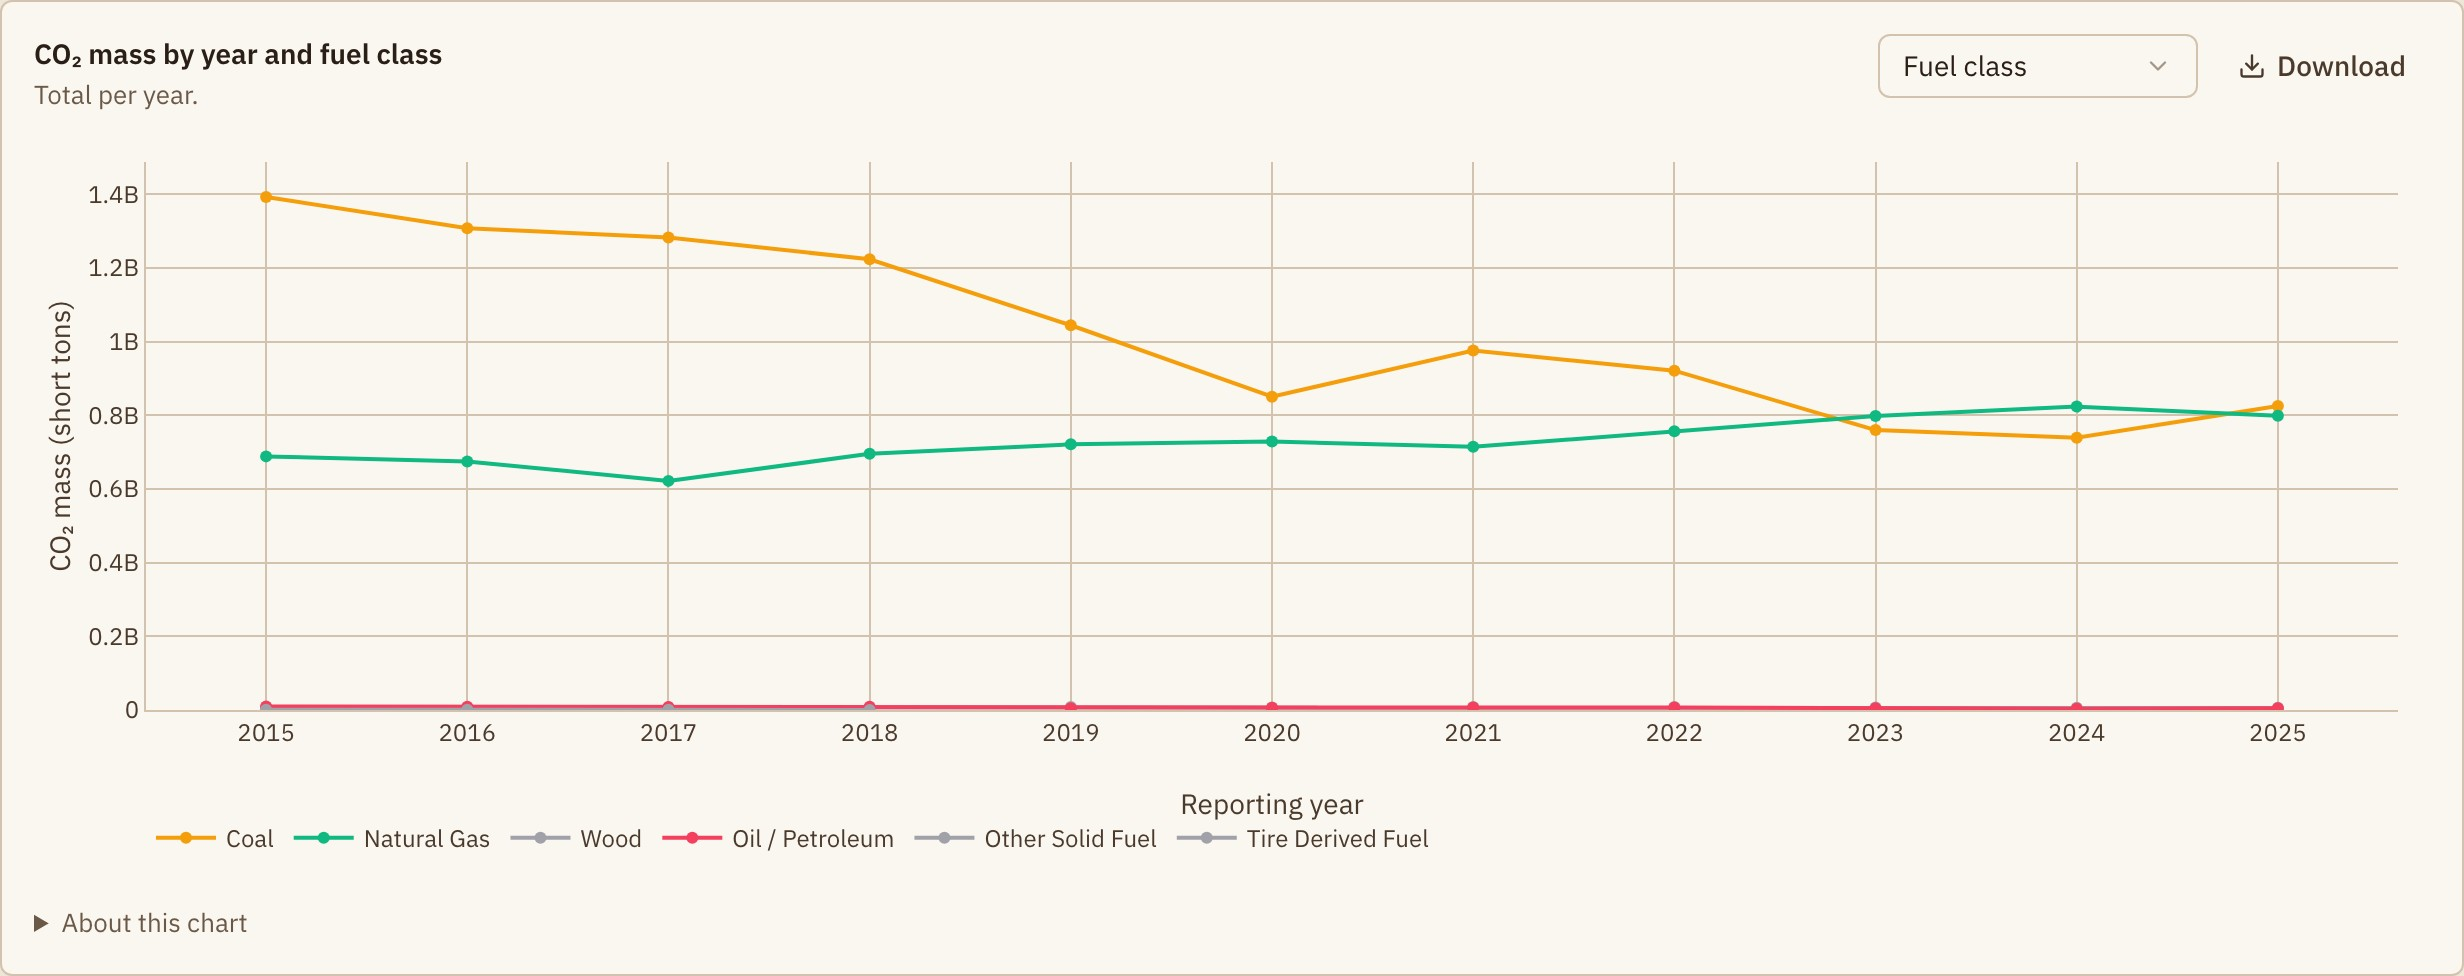
\includegraphics[width=\linewidth]{p2-trend.jpg}
  \caption{Trend chart: total \COtwo{} per year from coal and natural-gas units, 2015--2025.}
  \label{fig:trend}
\end{figure}

\subsection{Q2: \NOx{} rate and post-combustion control}

Figure~\ref{fig:box} shows the \NOx{} emission rate by fuel class on a log scale. Gas units have
a median of 0.034~lb/MMBtu (IQR 0.013--0.096), coal units 0.136 (0.082--0.219), and oil units
0.574 (0.188--1.20), with wide overlap within each fuel.

\begin{figure}[!htbp]
  \centering
  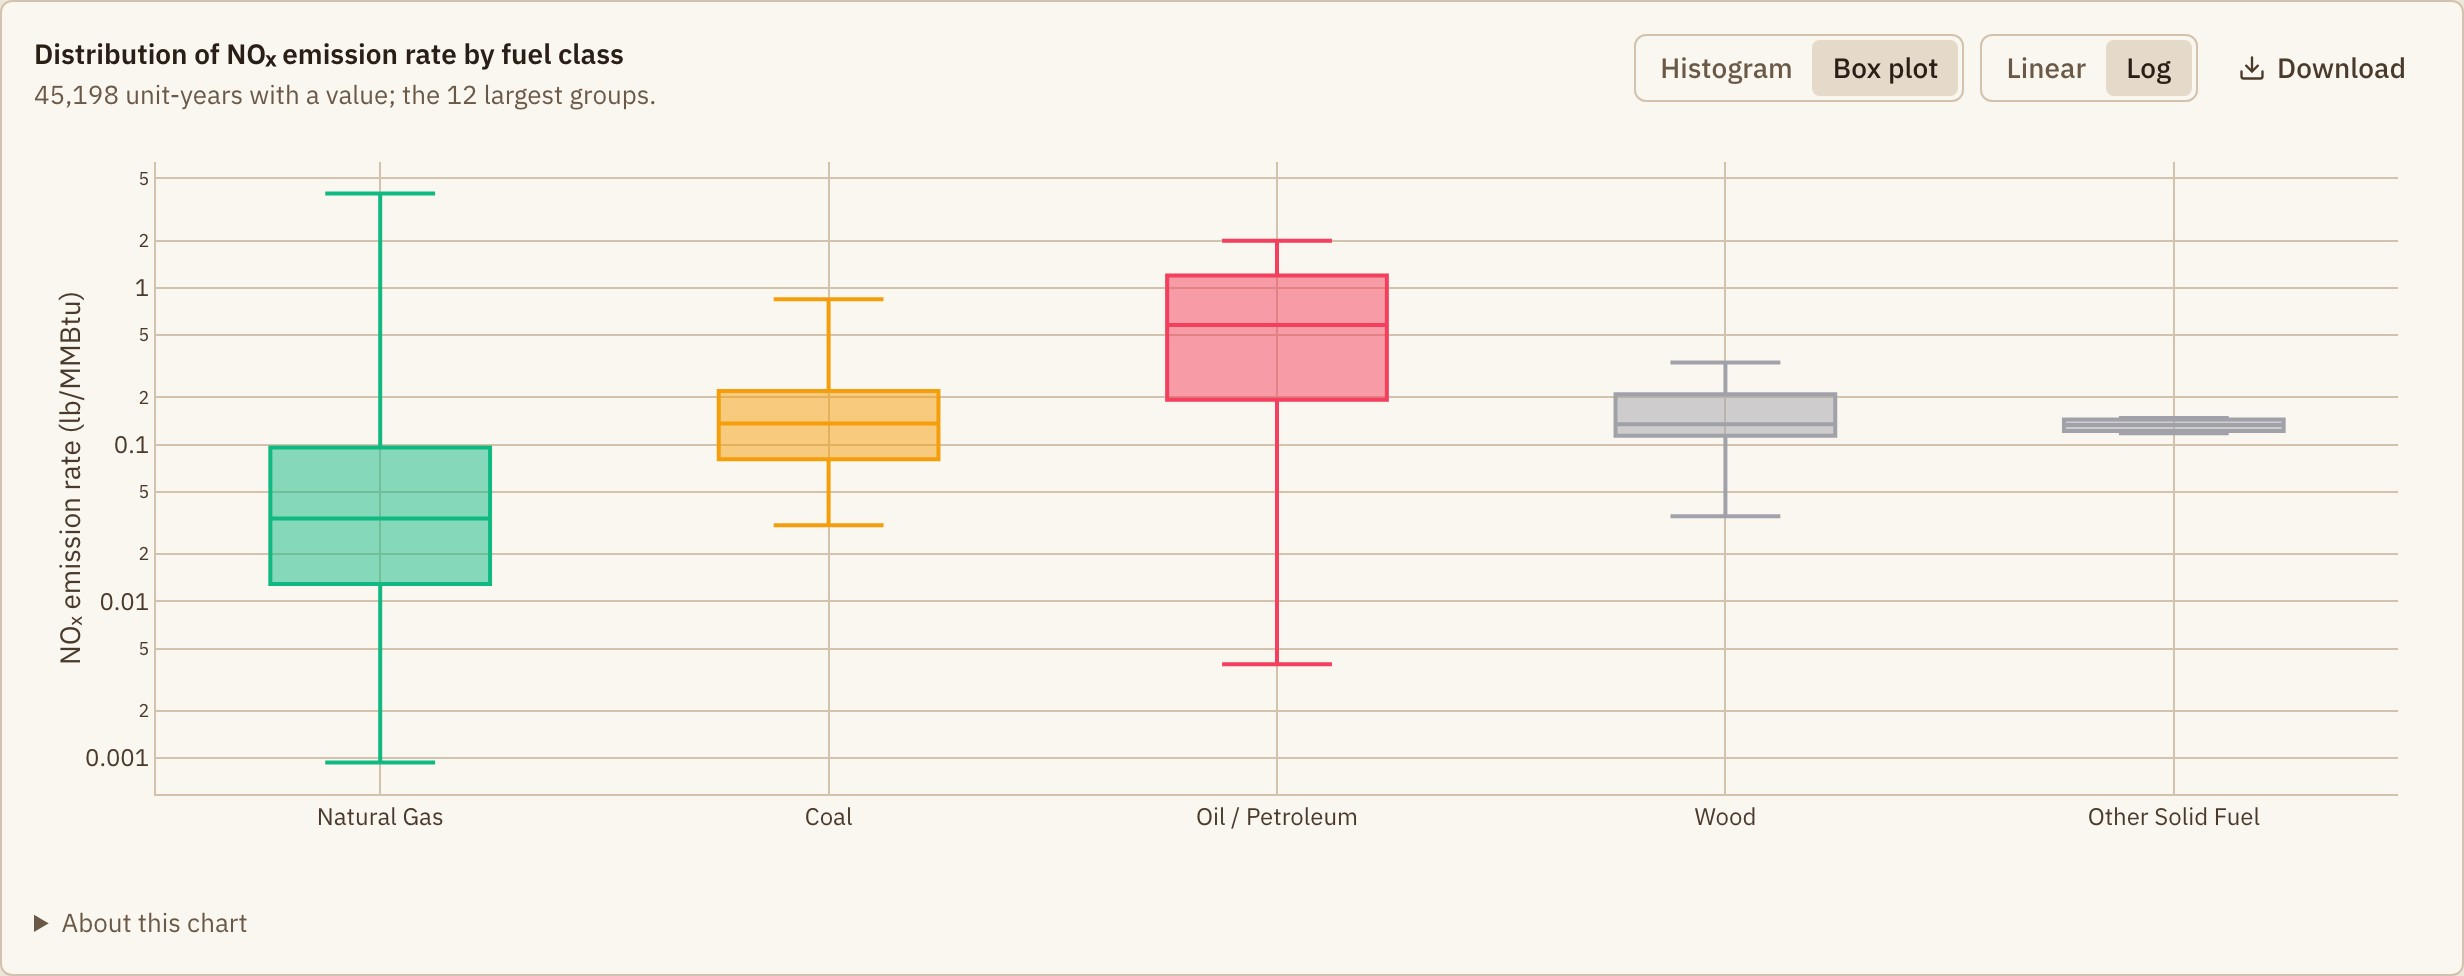
\includegraphics[width=\linewidth]{p2-box.jpg}
  \caption{Box plot of the \NOx{} emission rate by fuel class (log scale).}
  \label{fig:box}
\end{figure}

In 2024, 1{,}548 unit-years that ran list SCR among their \NOx{} controls and 487 list no \NOx{}
control.
The rate is defined (\NOx{} mass reported and heat input above zero) for 1{,}547 and 479 of them.
Their pooled rates are 0.037 and 0.159~lb/MMBtu, so units without control emit at a 330\,\%
higher rate; the medians are 0.012 and 0.305 (Figure~\ref{fig:compare}). Welch's test
($t = -22.3$, $p < 0.001$) and the Mann--Whitney test ($z = -29.8$, $p < 0.001$) both reject
equal groups. The difference is real, but not all of it is due to SCR, because the two groups
are different fleets: 874 of the 1{,}548 SCR unit-years are combined-cycle units, while the
487 uncontrolled unit-years are mostly gas and oil units (283 gas and 180 oil). A fairer comparison holds fuel and unit type fixed, which the Compare groups tab supports by
adding those filters.

\begin{figure}[!htbp]
  \centering
  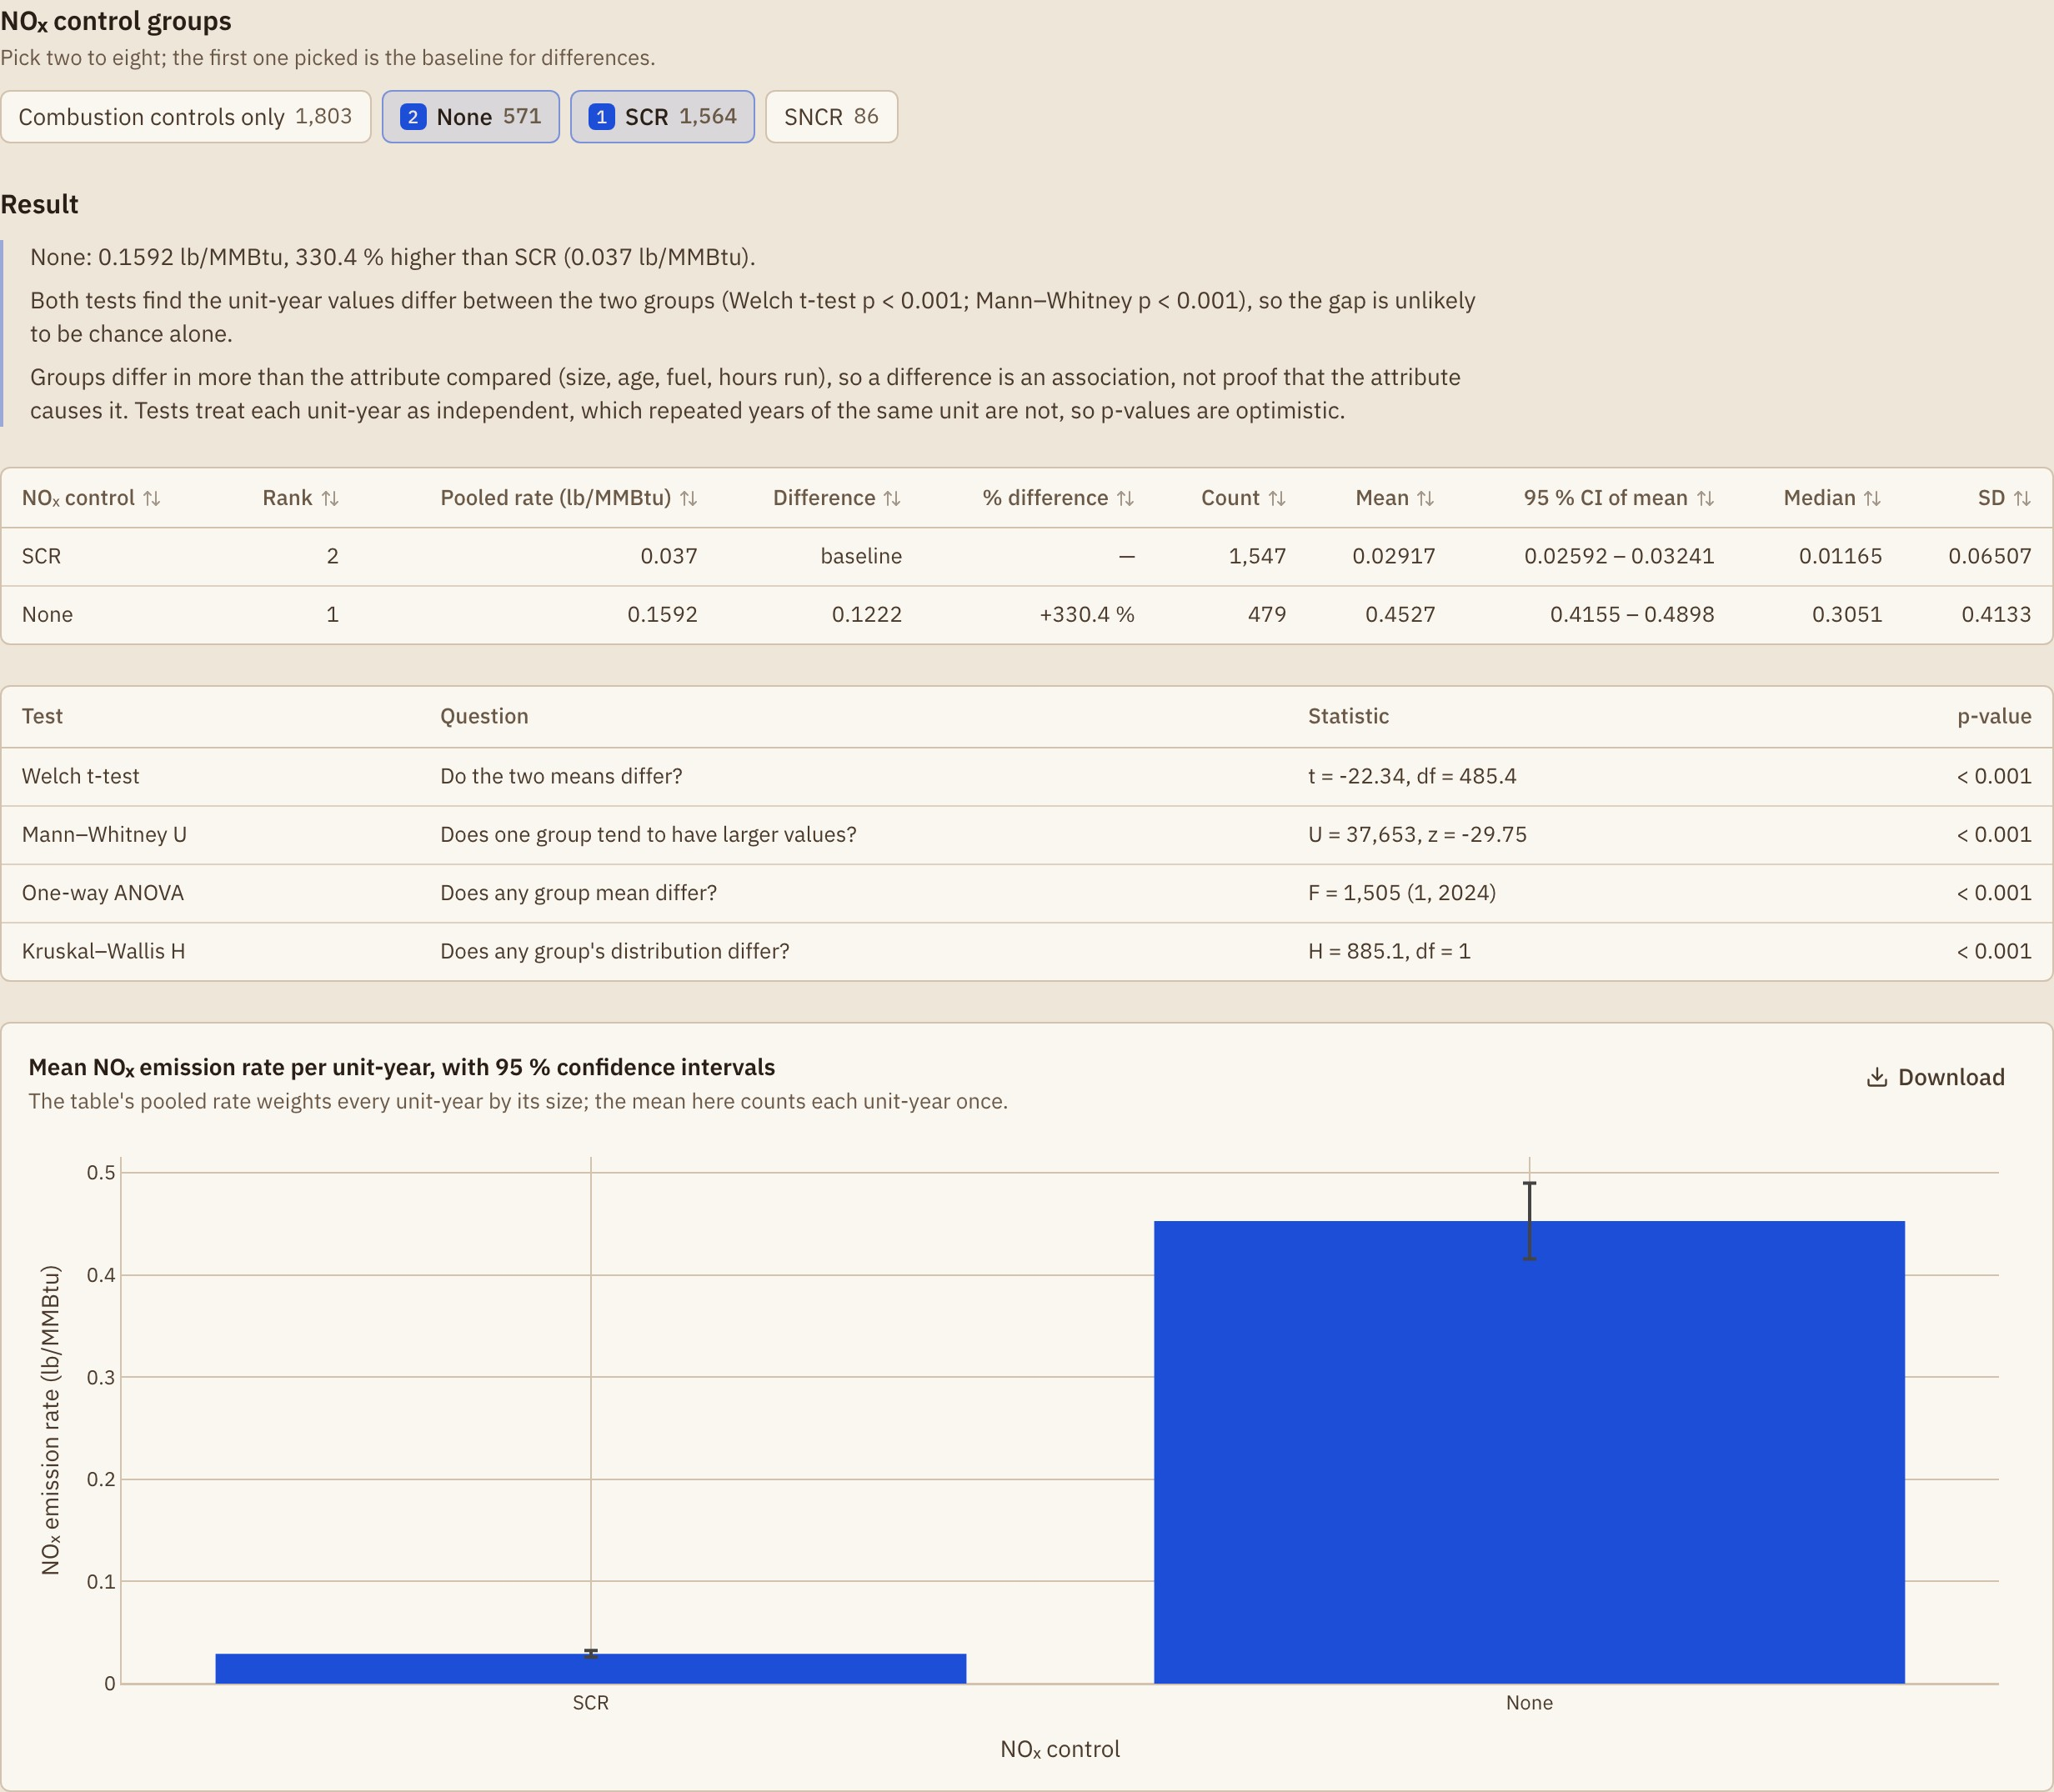
\includegraphics[width=\linewidth]{p2-compare.jpg}
  \caption{Compare groups tab: \NOx{} emission rate of units with SCR and with no \NOx{} control, 2024.}
  \label{fig:compare}
\end{figure}

\paragraph{Unusual observations.} Over 2015--2025, 3{,}582 unit-years lie above the far-out fence
for \NOx{} intensity (6.1~lb/MWh, against a median of 0.58). Of these, 3{,}491 are combustion
turbines with a median operating time of 42~hours a year: peaking units whose start-ups emit
\NOx{} with almost no generation. They are real reports, not errors, and they are why the pooled
rate (0.70~lb/MWh) is a better summary than the mean (2.46).

\paragraph{A misleading correlation.} The Pearson correlation between \COtwo{} intensity and heat
rate over the 37{,}718 unit-years reporting both is 0.9998, while Spearman's rank correlation is
0.765 (Figure~\ref{fig:correlation}). A few unit-years with tiny gross loads have intensities
and heat rates thousands of times the norm. They dominate Pearson's $r$ and barely affect the
ranks, so Spearman's $\rho$ is the better summary for these heavy-tailed variables. This is why
the chart offers both.

\begin{figure}[!htbp]
  \centering
  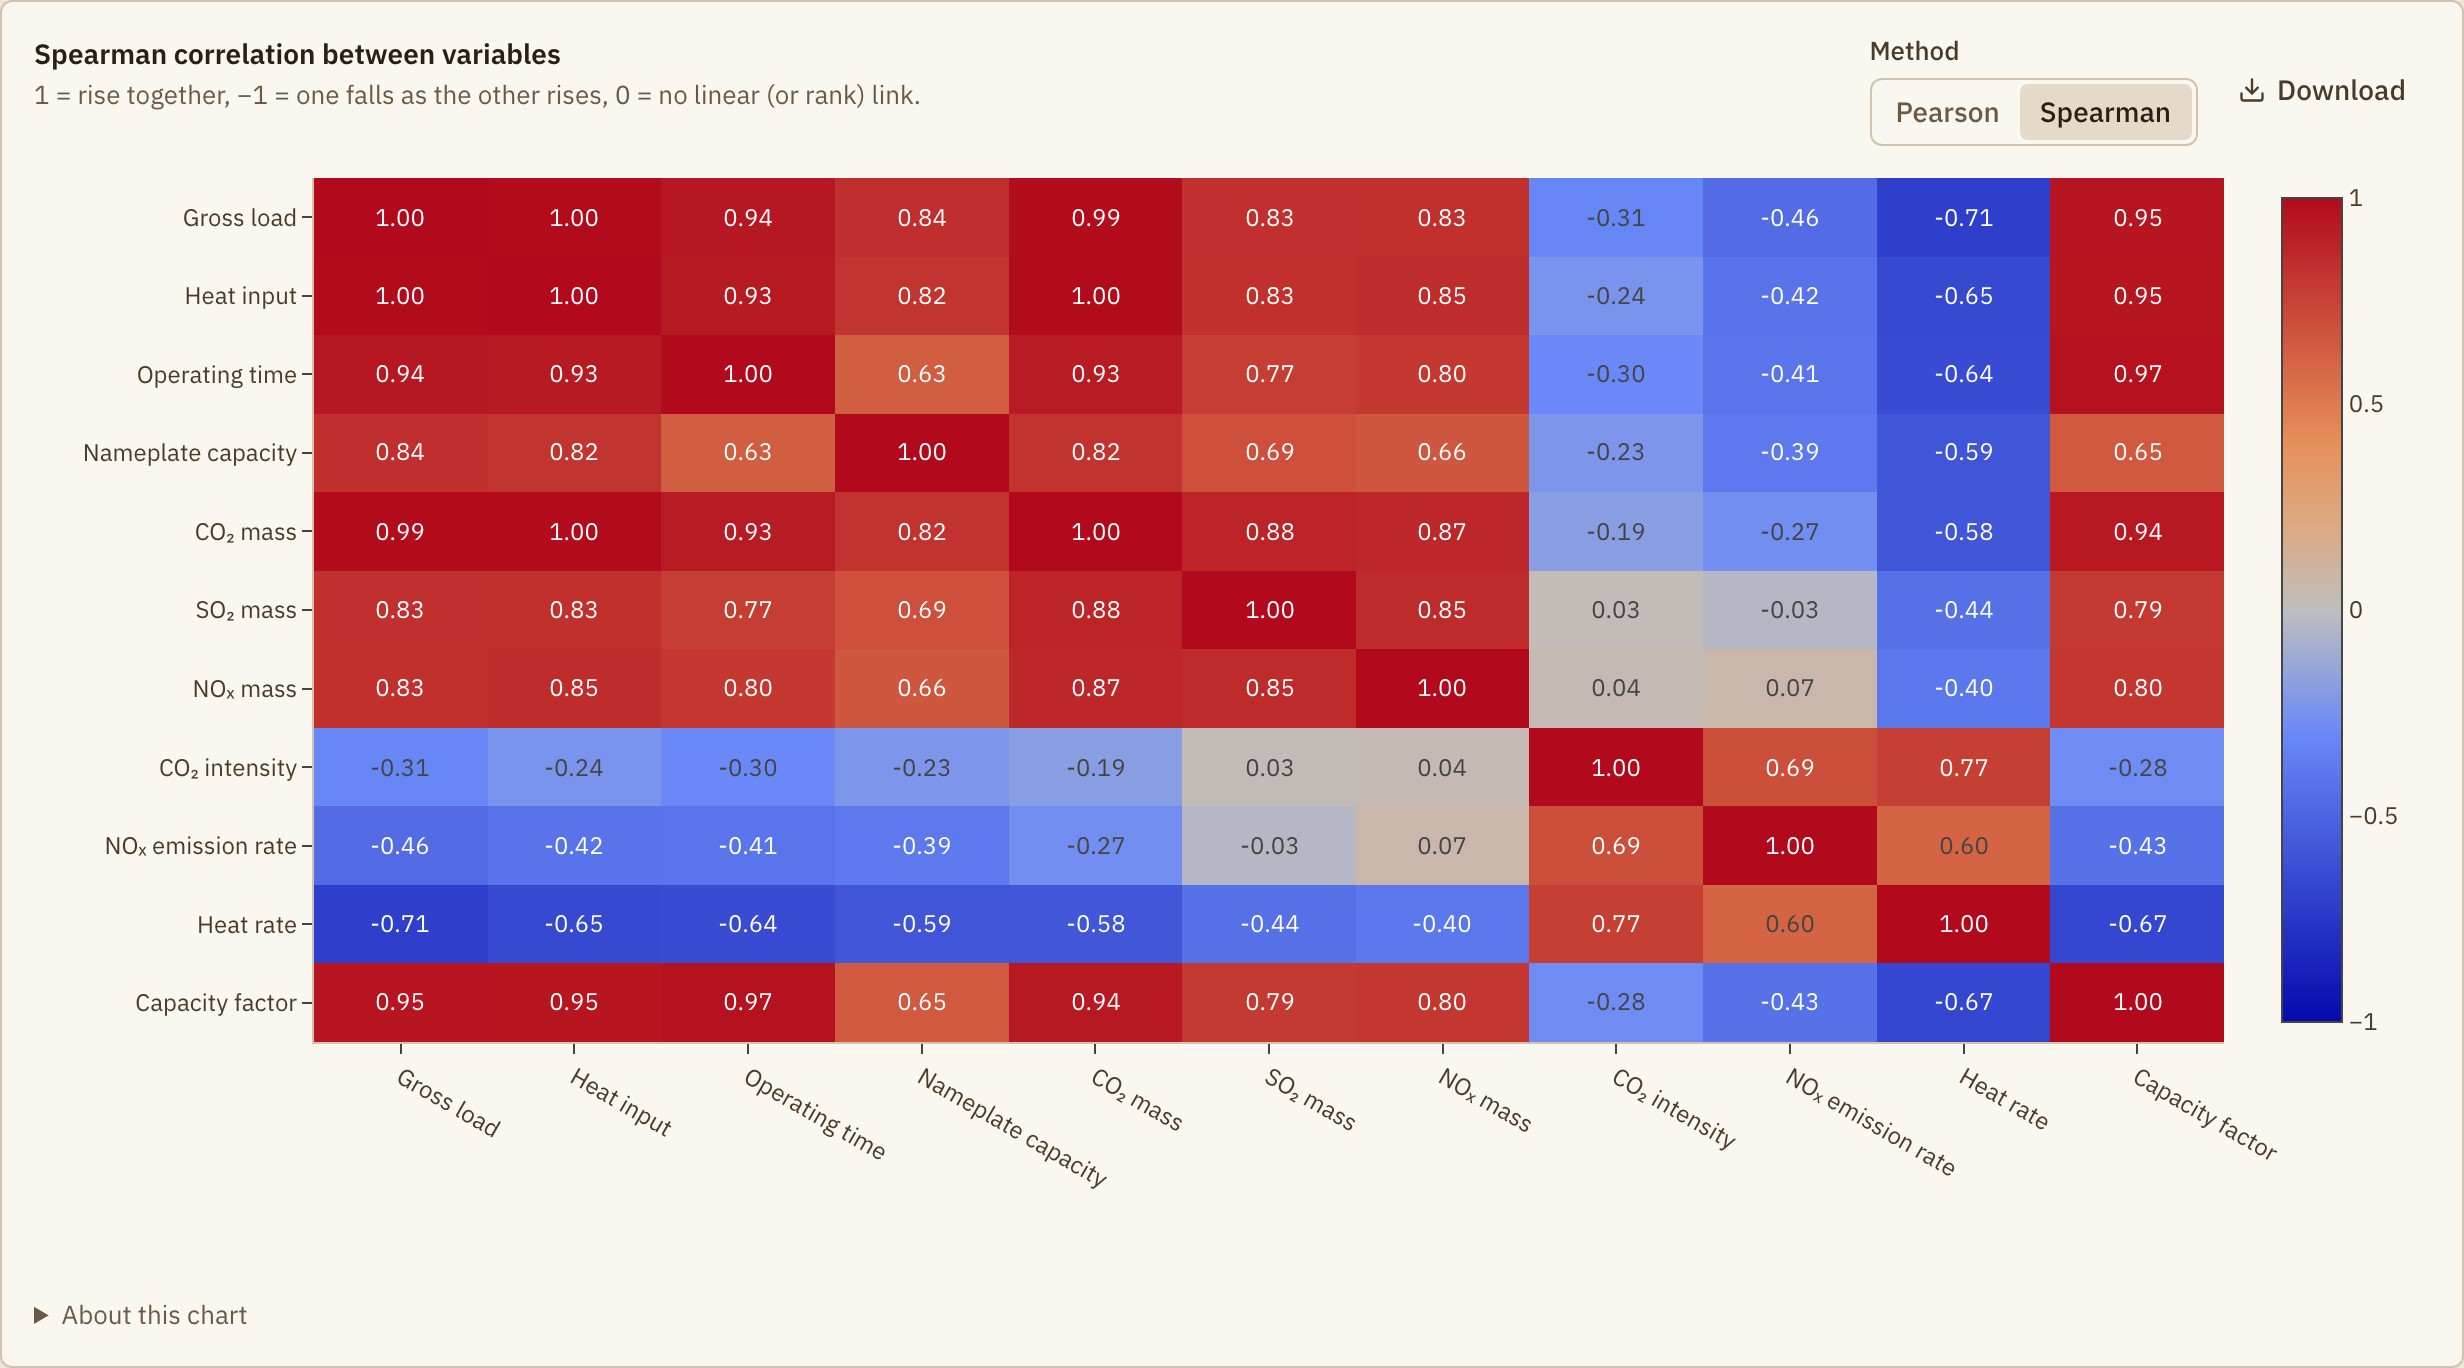
\includegraphics[width=0.85\linewidth]{p2-correlation.jpg}
  \caption{Spearman correlation heat map of eleven variables, 2015--2025.}
  \label{fig:correlation}
\end{figure}

\subsection{Q3: impacts by state}

In 2024 Texas contributed the most to every category: $1.91 \times 10^{11}$~kg \COtwo{}~eq of
global warming and $1.34 \times 10^{8}$~kg \SOtwo{}~eq of acidification, followed for
acidification by Missouri ($7.93 \times 10^{7}$) and Kentucky ($5.65 \times 10^{7}$)
(Figure~\ref{fig:impacts}). Per MWh the order changes: Nebraska (2.32~kg \SOtwo{}~eq/MWh), North
Dakota (1.83), and Missouri (1.57) lead. Coal units produced 93\,\% of the reported gross load
of Nebraska and North Dakota and 83\,\% of Missouri's, against 20\,\% in Texas, whose pooled
\SOtwo{} intensity was 0.51~lb/MWh against Nebraska's 3.95. Totals show where impacts occur;
intensities show how clean a state's generation is.

\begin{figure}[!htbp]
  \centering
  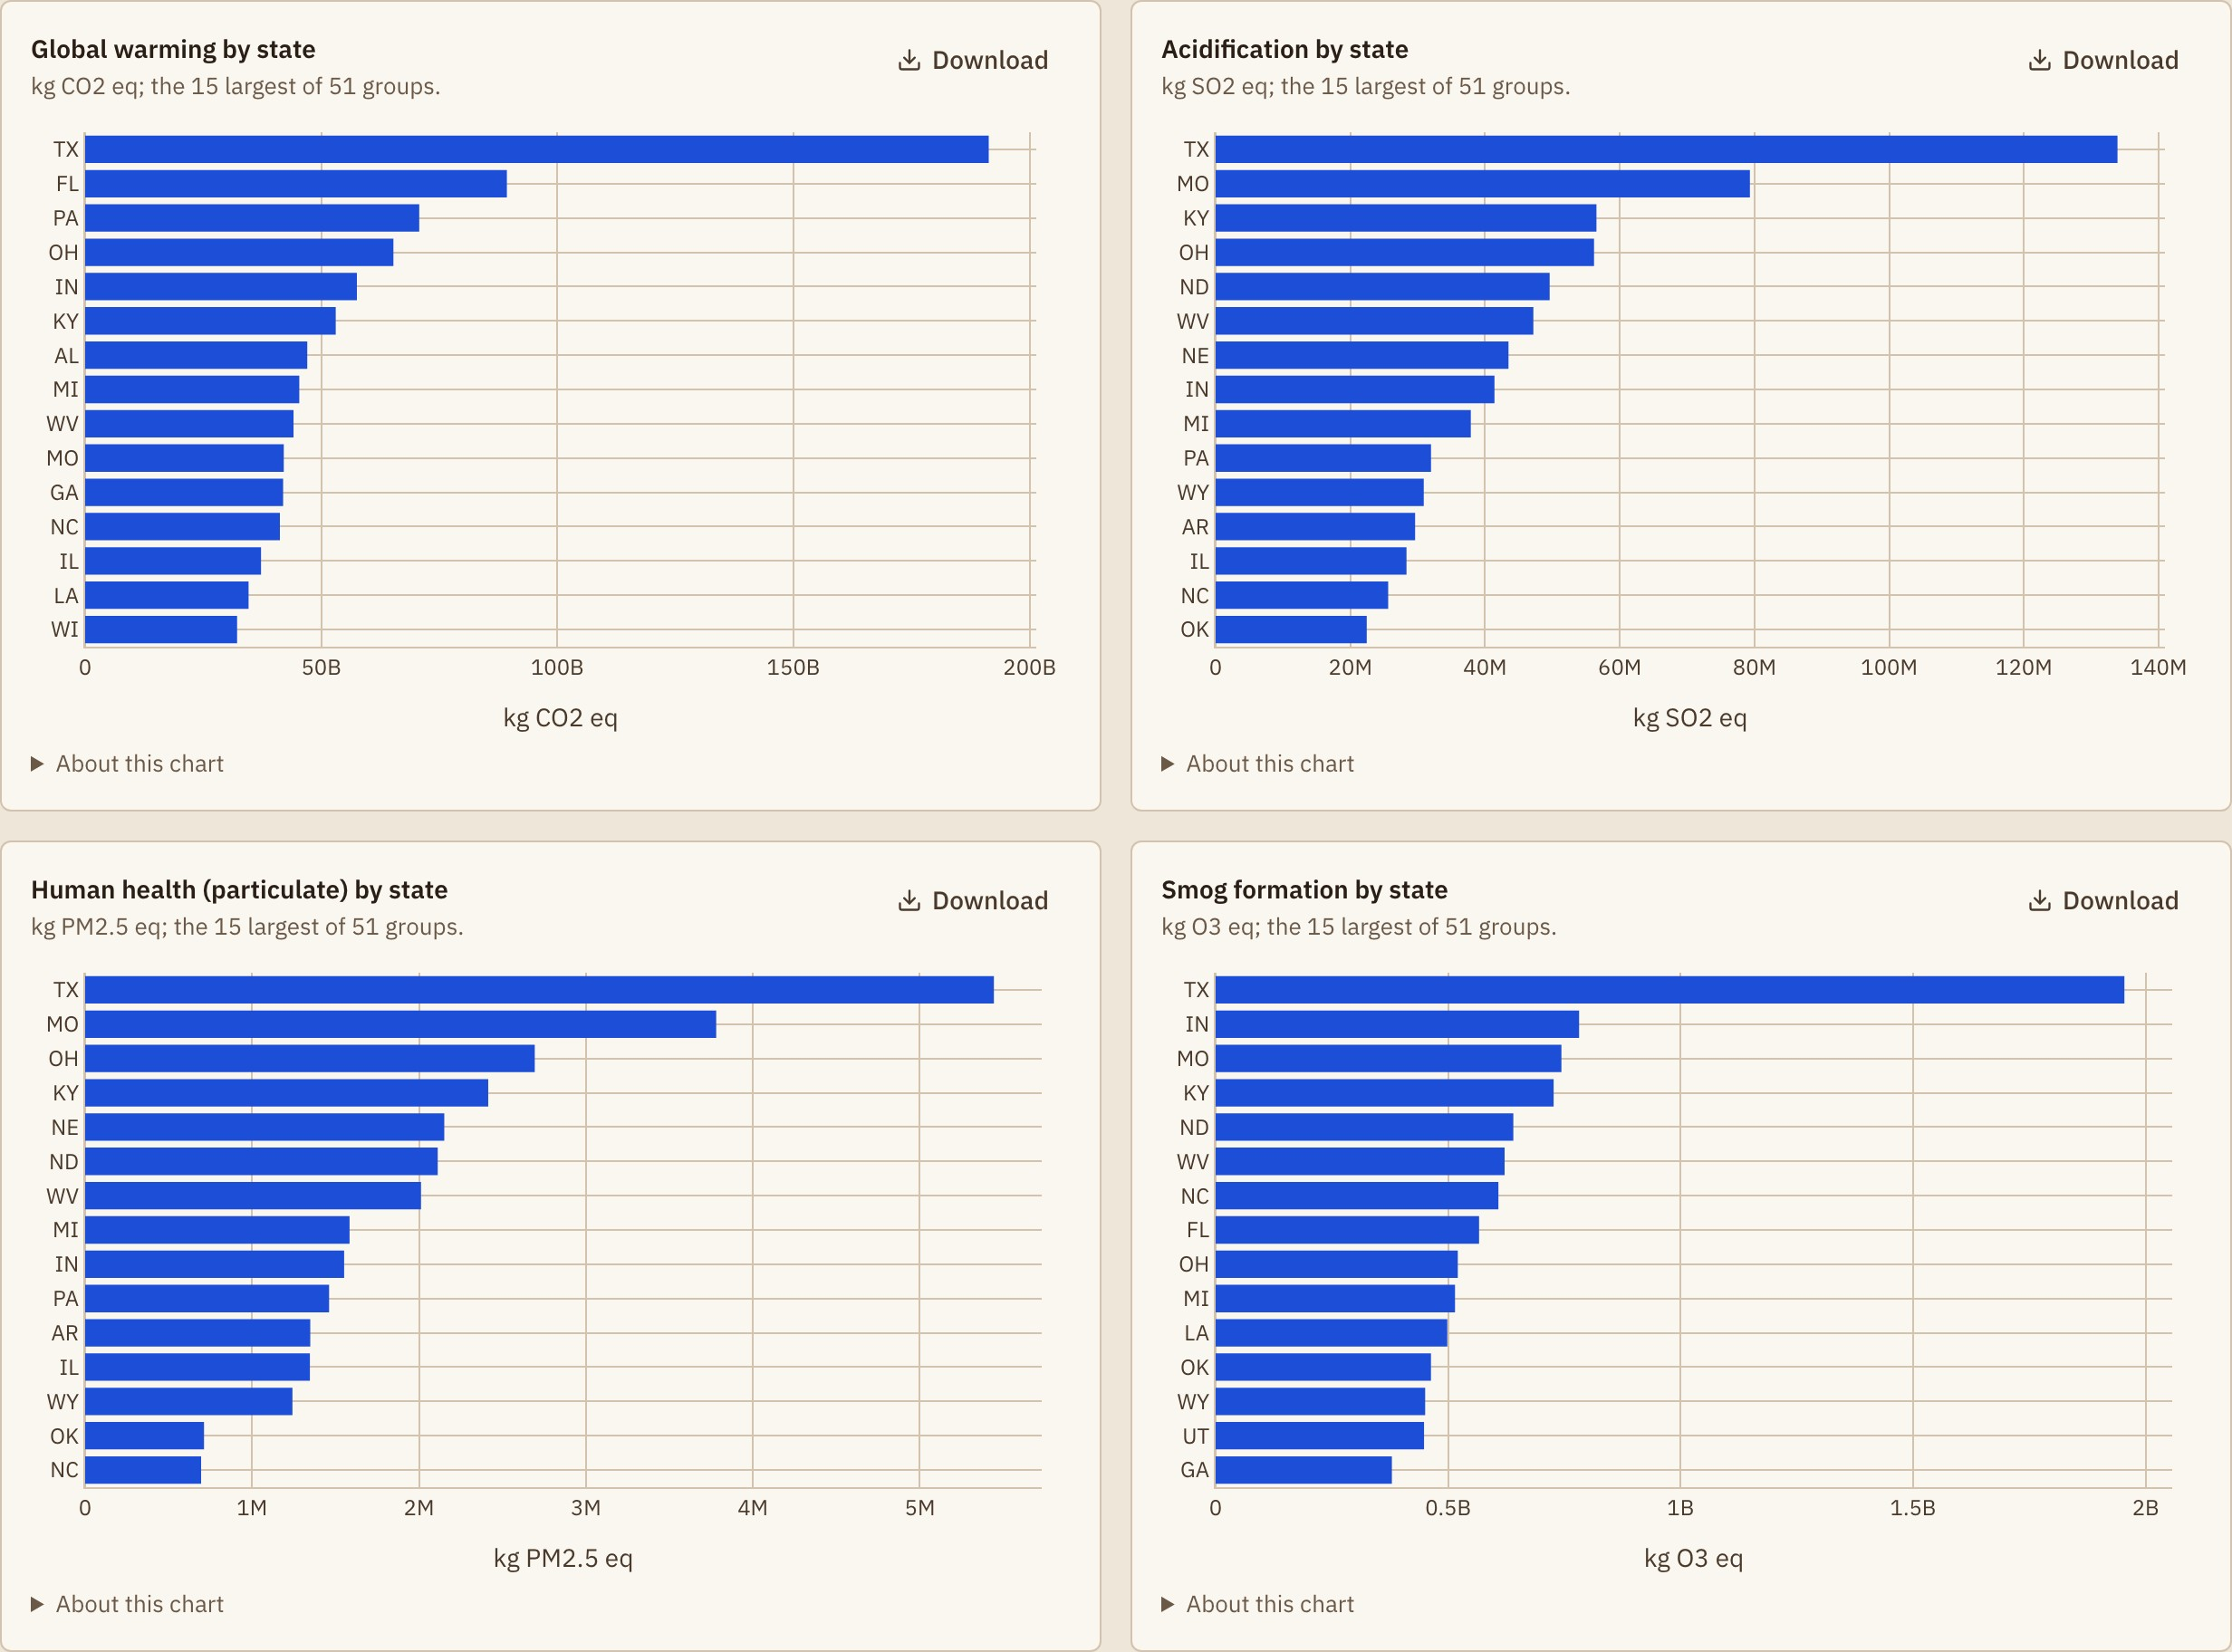
\includegraphics[width=\linewidth]{p2-impacts.jpg}
  \caption{TRACI impacts tab: TRACI categories by state for 2024, each in its own unit (the 15
  largest states per category).}
  \label{fig:impacts}
\end{figure}

\subsection{Q4: prediction}

Table~\ref{tab:models} compares the models. Both trained models beat the median baseline by a
wide margin on the test years: Ridge lowers the MAE by 47\,\% and the tree by 76\,\%, and the
intervals do not overlap. The tree's training ($R^2 = 0.956$), validation, and test results are
close, so it does not noticeably overfit despite its depth. Without same-year heat input, gross
load, and operating time, validation $R^2$ falls from 0.853 to 0.704 for Ridge and from 0.967 to
0.837 for the tree. Most of the remaining accuracy comes from the previous year's \NOx{} rate,
which reflects the unit's combustion technology and controls.

The persistence reference is more accurate than both models. Its test MAE is 18.5~tons
(16.1--21.2), against 26.3 for the tree; the tree's MAE is 7.8~tons higher (6.3--9.4), and
Ridge's 40.0~tons higher (35.8--44.8). Persistence also wins without same-year activity, where
last year's tons reach a validation $R^2$ of 0.884 against the tree's 0.837. The reason is
physical: \NOx{} mass is the emission rate times heat input, and a unit's rate changes little from
one year to the next. A tree can approximate that product only in steps, and Ridge on the log
scale gives the previous rate a linear rather than a logarithmic effect.

We tried three reformulations that build the product into the model, each tuned on the
validation years and scored once on the test years (\code{ml/reformulations.py}): the
persistence estimate as an extra input (test MAE: tree 21.3, Ridge 25.0~tons); predicting this
year's rate and multiplying by heat input (tree 20.2, Ridge 44.8); and predicting a correction
to the persistence estimate (tree 19.7, Ridge 22.4). None beats persistence: the inputs carry
little information about \emph{changes} in a unit's rate. One likely cause of such changes, a
control installed or retired, is invisible to the models, which see this year's controls but not
last year's, so they cannot tell a new control from one the previous rate already reflects.

The models are therefore not the best point forecast of next year's \NOx{}. What they add is a
response to inputs that persistence ignores: persistence scales only with heat input, while the
models also respond to load, controls, fuel, and unit type, which is what the What-if scenarios
need. Those responses are associations learned across units, not measured effects, as the
scenarios below show.

\begin{table}[H]
  \centering\small
  \setlength{\tabcolsep}{4.5pt}
  \caption{\NOx{} models: validation (2022--2023) and test (2024--2025) results, with 95\,\%
  cluster-bootstrap intervals for test MAE and $R^2$. Ablation: validation $R^2$ without
  same-year heat input, gross load, and operating time. Persistence is a reference, not a
  registered model.}\label{tab:models}
  \begin{tabular}{@{}lrrrrrrr@{}}
    \toprule
    & \multicolumn{2}{c}{\textbf{Validation}} & \multicolumn{4}{c}{\textbf{Test}} & \textbf{Ablation}\\
    \cmidrule(lr){2-3}\cmidrule(lr){4-7}\cmidrule(l){8-8}
    \textbf{Model} & MAE (t) & $R^2$ & MAE (t) & RMSE (t) & $R^2$ & MAPE & $R^2$\\
    \midrule
    Baseline (median) & 114.2 & 0.474 & 109.4 & 366.9 & 0.489 & 143.6\,\% & 0.474\\
    & & & \scriptsize 99.3--121.0 & & \scriptsize 0.443--0.538 & & \\
    Ridge ($\alpha = 10$) & 57.9 & 0.853 & 58.5 & 213.5 & 0.827 & 49.3\,\% & 0.704\\
    & & & \scriptsize 52.7--64.9 & & \scriptsize 0.784--0.870 & & \\
    Tree (depth $\le 20$, leaf 20) & 26.5 & 0.967 & 26.3 & 113.9 & 0.951 & 20.9\,\% & 0.837\\
    & & & \scriptsize 23.4--29.7 & & \scriptsize 0.937--0.963 & & \\
    \midrule
    Persistence (reference) & 18.7 & 0.965 & 18.5 & 92.8 & 0.967 & 15.3\,\% & 0.884\\
    & & & \scriptsize 16.1--21.2 & & \scriptsize 0.953--0.979 & & \\
    \bottomrule
  \end{tabular}
\end{table}

\begin{figure}[!htbp]
  \centering
  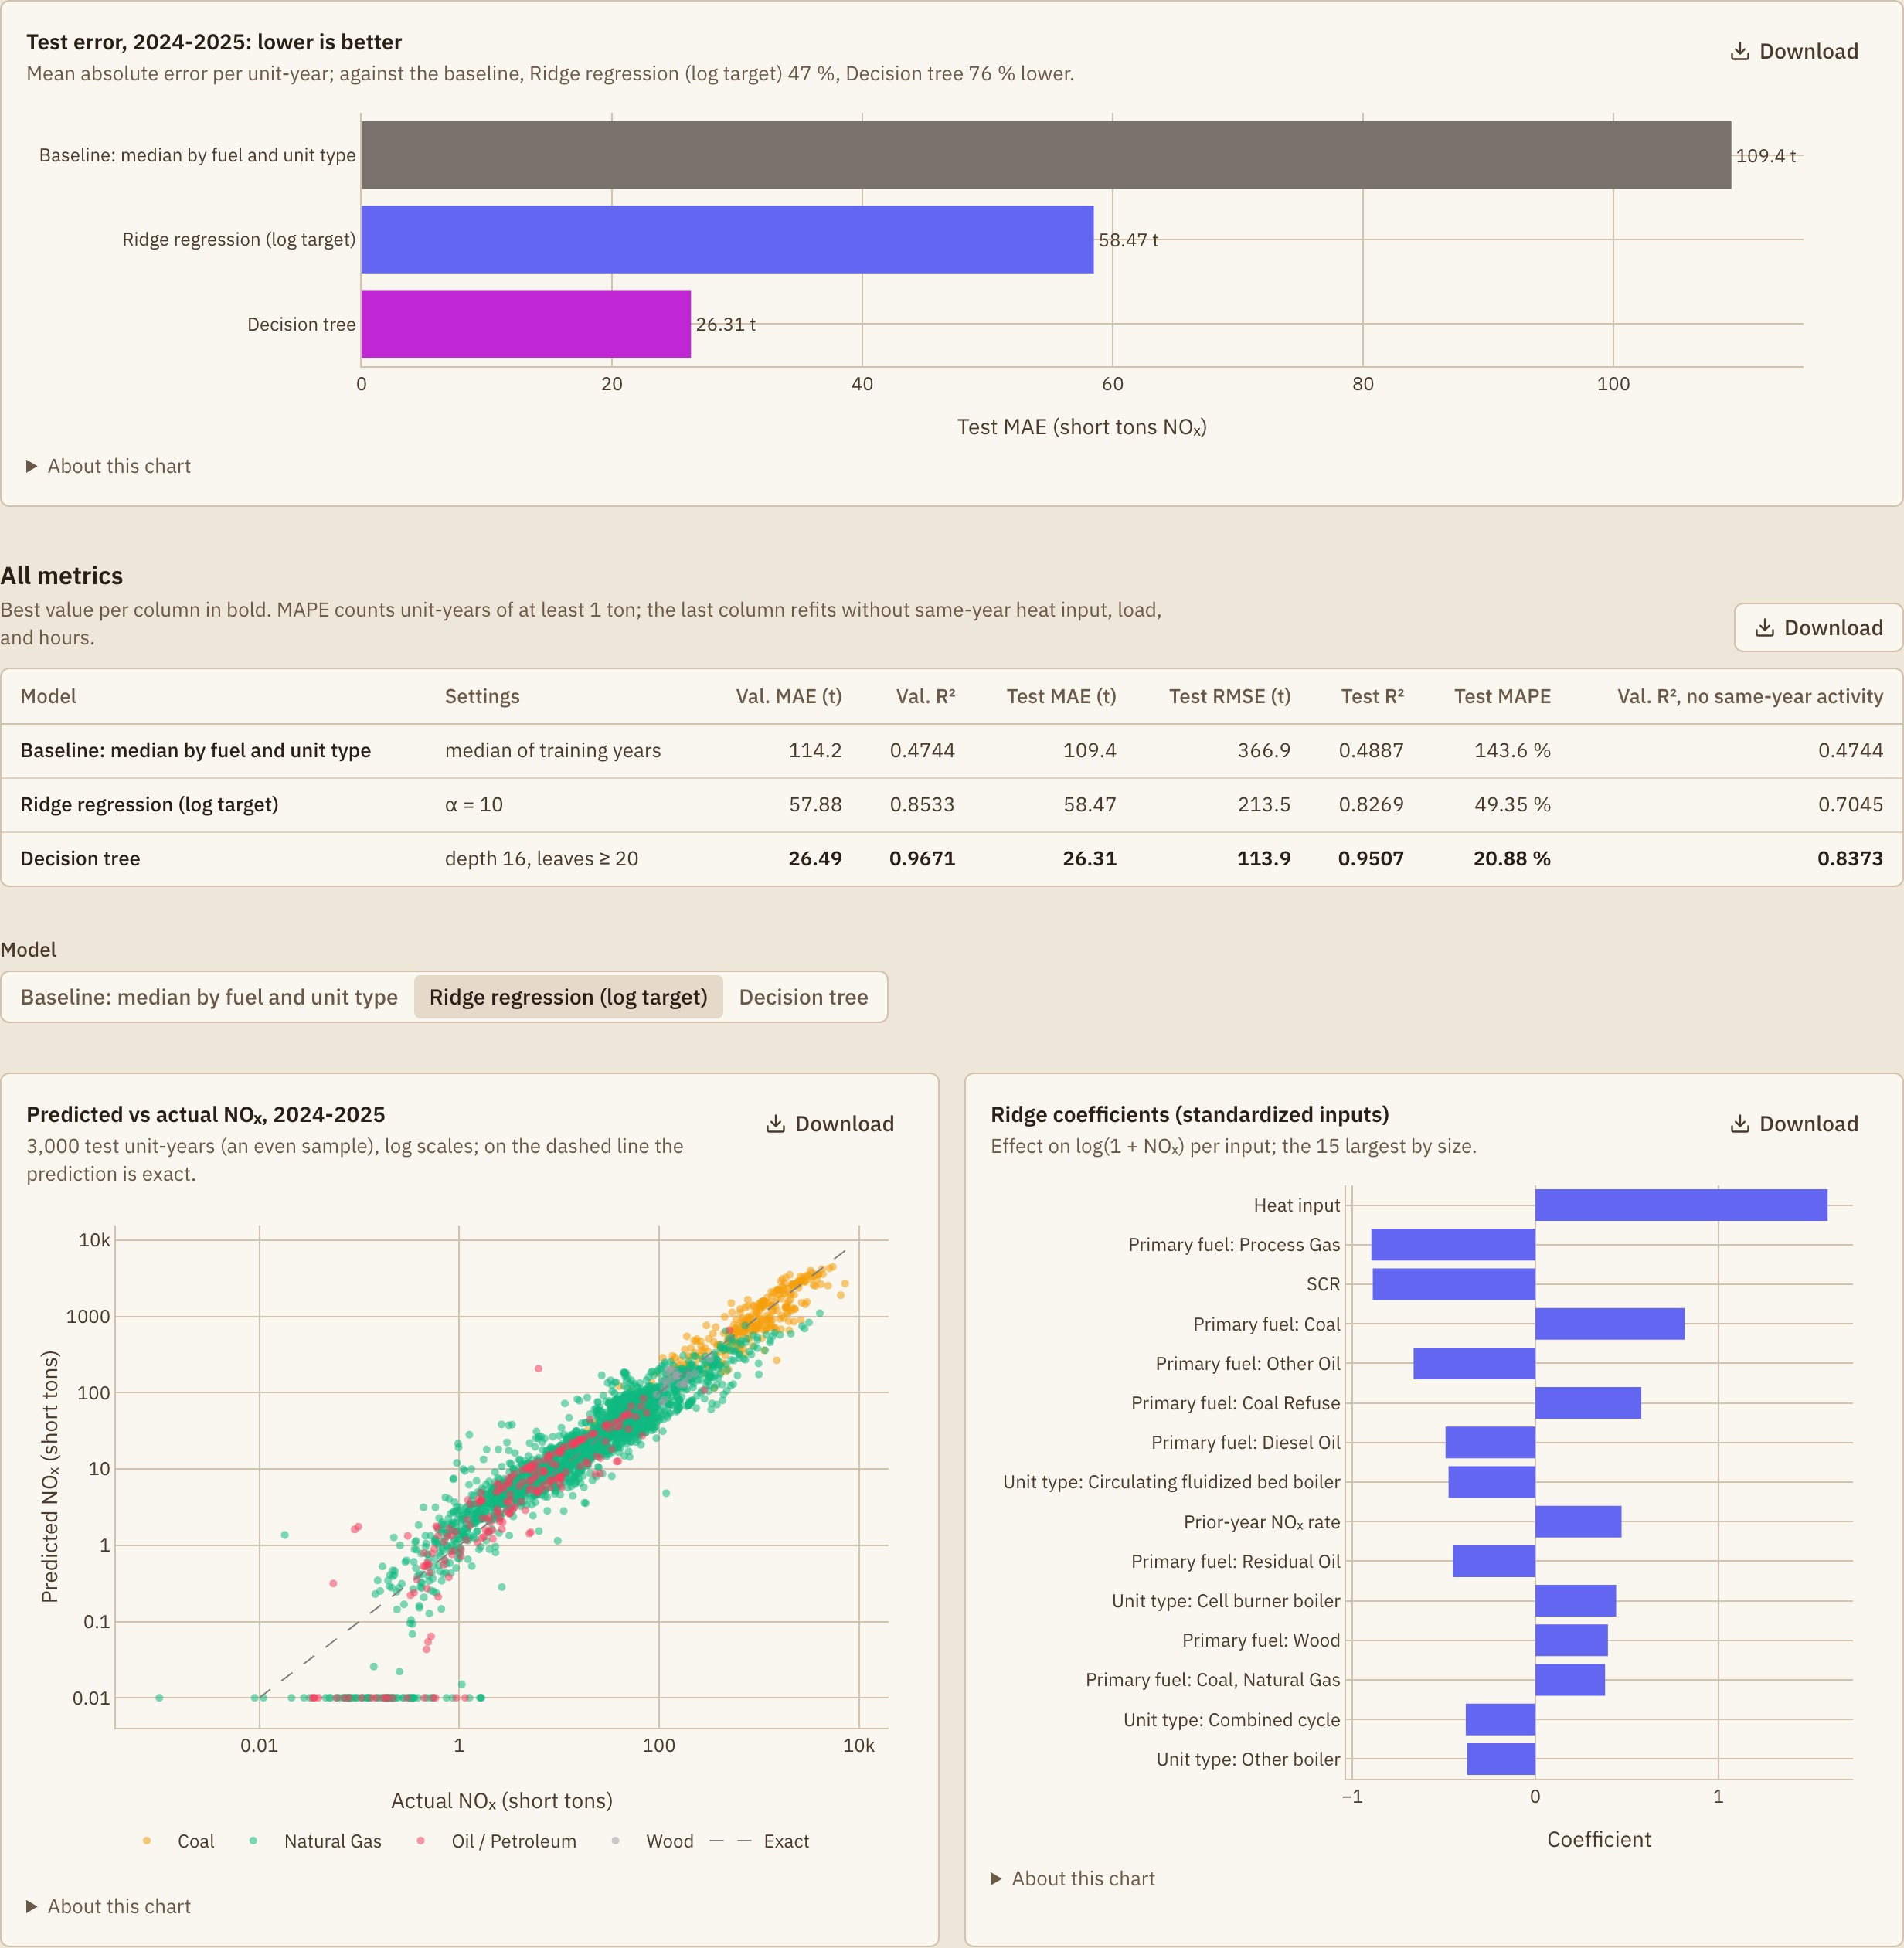
\includegraphics[width=\linewidth]{p2-models.jpg}\\[4pt]
  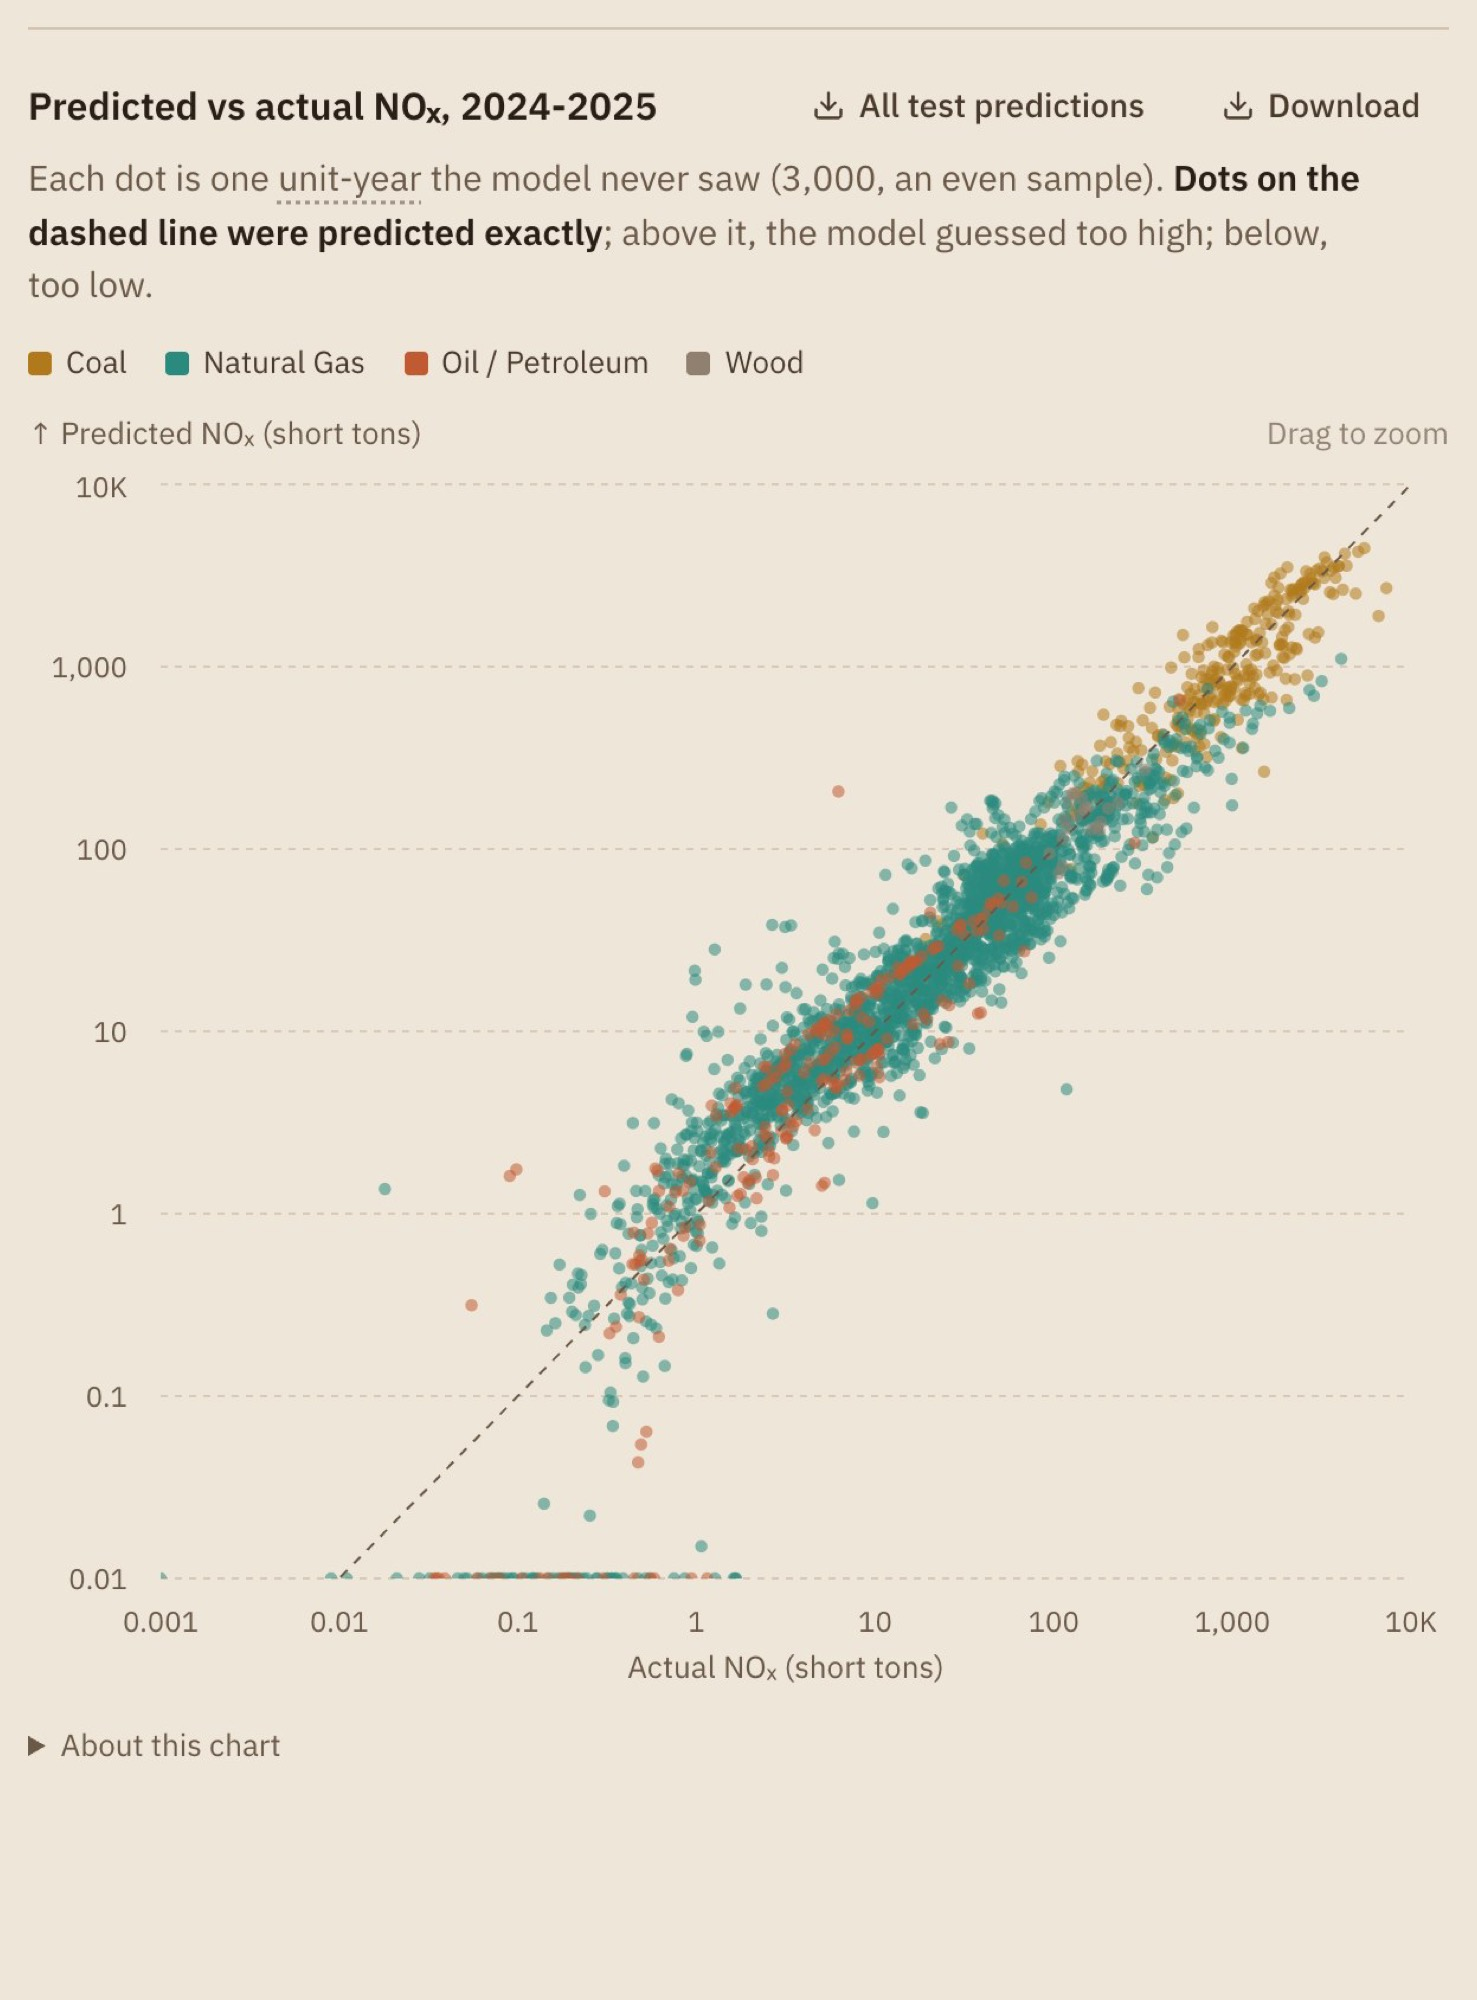
\includegraphics[width=\linewidth]{p2-predicted.jpg}
  \caption{Models tab. Top: test MAE and $R^2$ of the three models with 95\,\% intervals. Bottom:
  predicted against actual \NOx{} for an even sample of 3{,}000 test unit-years (log scales) and
  the tree's feature importances.}
  \label{fig:models}
\end{figure}

\paragraph{Where the errors are.} The error is concentrated in a few large units. Coal units are
789 of the 7{,}755 test unit-years (10\,\%), but the tree's MAE on them is 166.9~tons against
11.1 for gas, 15.8 for wood, and 2.6 for oil units, so coal accounts for about 65\,\% of the
tree's total absolute error. On average the tree under-predicts coal units by 31.7~tons, and Ridge
by 57.0 (Figure~\ref{fig:errors}, drawn from the 3{,}000-unit-year sample, shows 169.6 and
42.6~tons for the tree). This is consistent with persistence's advantage: the largest units are
where a change in a unit's emission rate costs the most tons, and the models see last year's rate
but not why it changed.

\begin{figure}[!htbp]
  \centering
  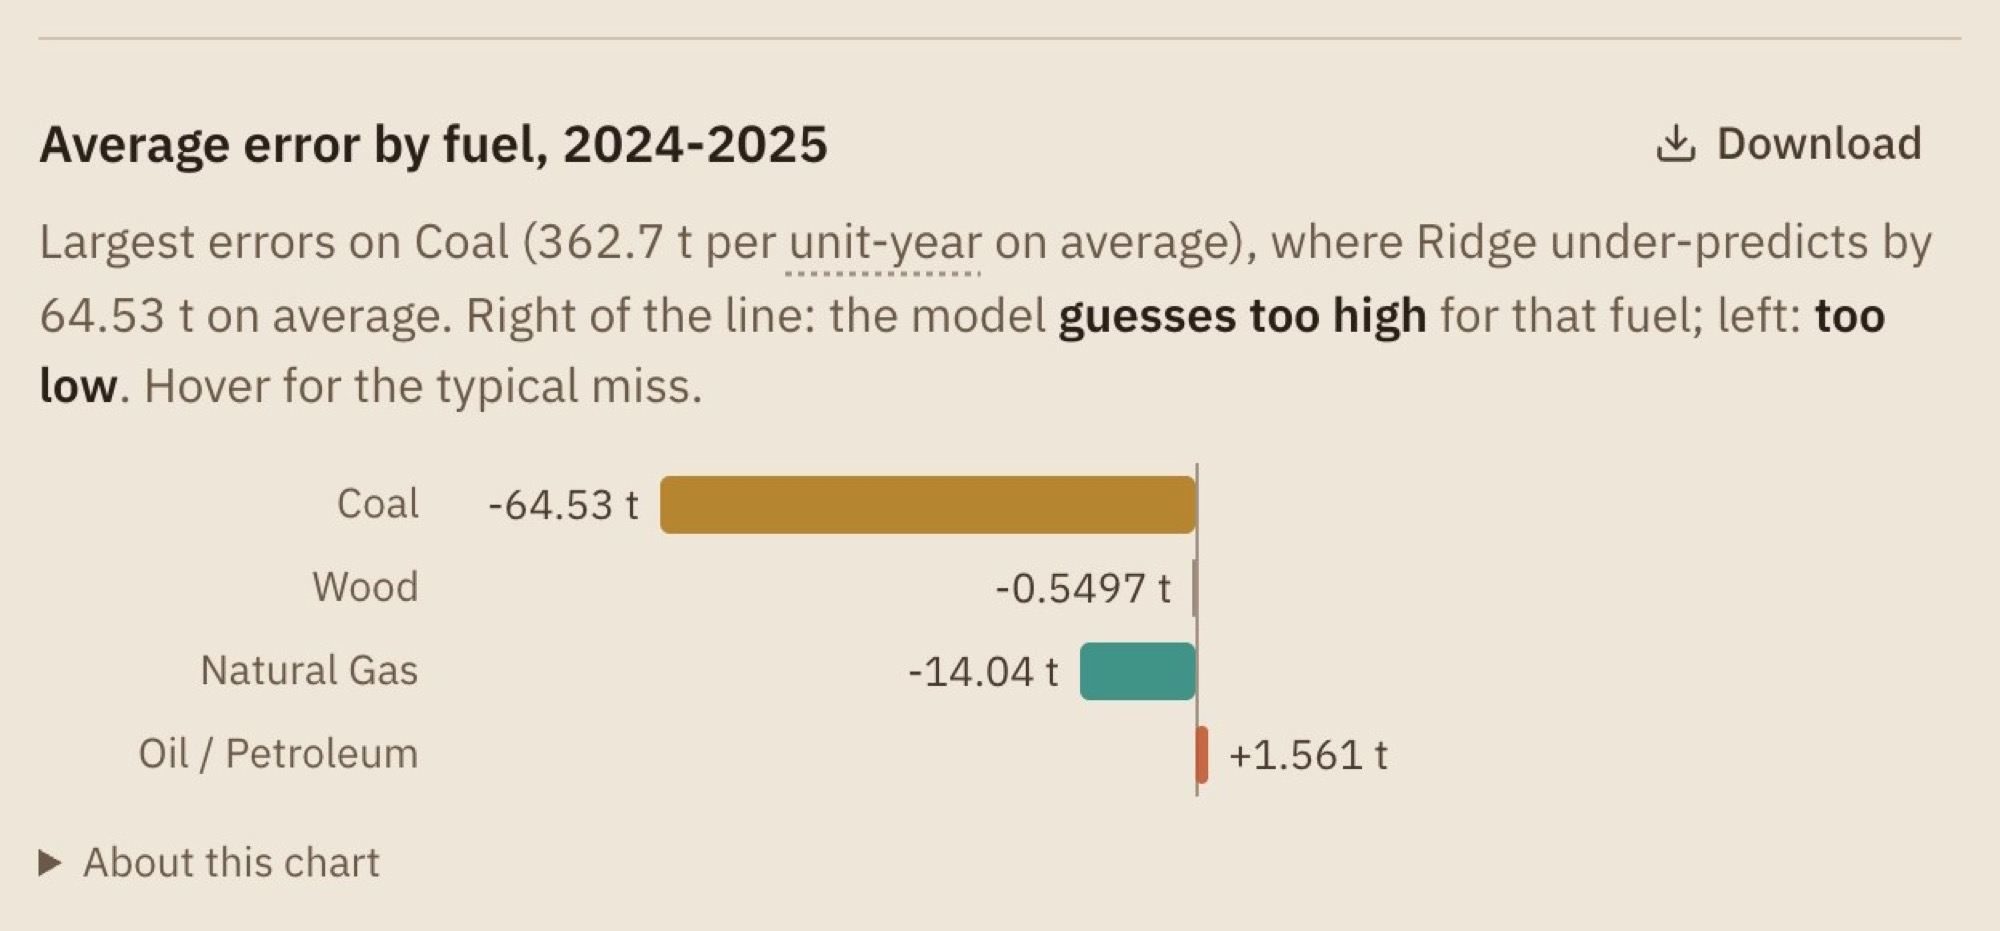
\includegraphics[width=0.6\linewidth]{p2-errors.jpg}
  \caption{Average signed error of the decision tree by fuel class, test years 2024--2025 (left of
  the line: under-prediction). Hovering a bar gives its mean absolute error.}
  \label{fig:errors}
\end{figure}

\paragraph{Sensitivity.} Figure~\ref{fig:sensitivity} varies the heat input of Ghent unit~2 in
2024, a 556~MW tangentially fired coal unit with low-\NOx{} burners and overfire air but no SCR.
It emitted 4{,}146 tons of \NOx{}. Both models under-predict this unit-year: Ridge predicts
2{,}972 tons and the tree 2{,}738. The reason is in the inputs: the unit's \NOx{} rate rose from
0.227~lb/MMBtu in 2023 to 0.314 in 2024, and the models rely on the previous year's rate. Raising
heat input by 50\,\% raises Ridge's prediction to 3{,}827 tons (29\,\%), an elasticity of about
0.6. The tree behaves differently: above about 33 million MMBtu its prediction stops rising
(about 3{,}500 tons), well inside the training range. A tree's prediction is a step function:
along this unit's path no split separates larger heat inputs, so more heat input changes
nothing. Beyond 85.8 million MMBtu, the largest heat input in the training years, the last five
of the 61 points enter the shaded region, and the reading above the chart says those predictions are
extrapolations.

\begin{figure}[!htbp]
  \centering
  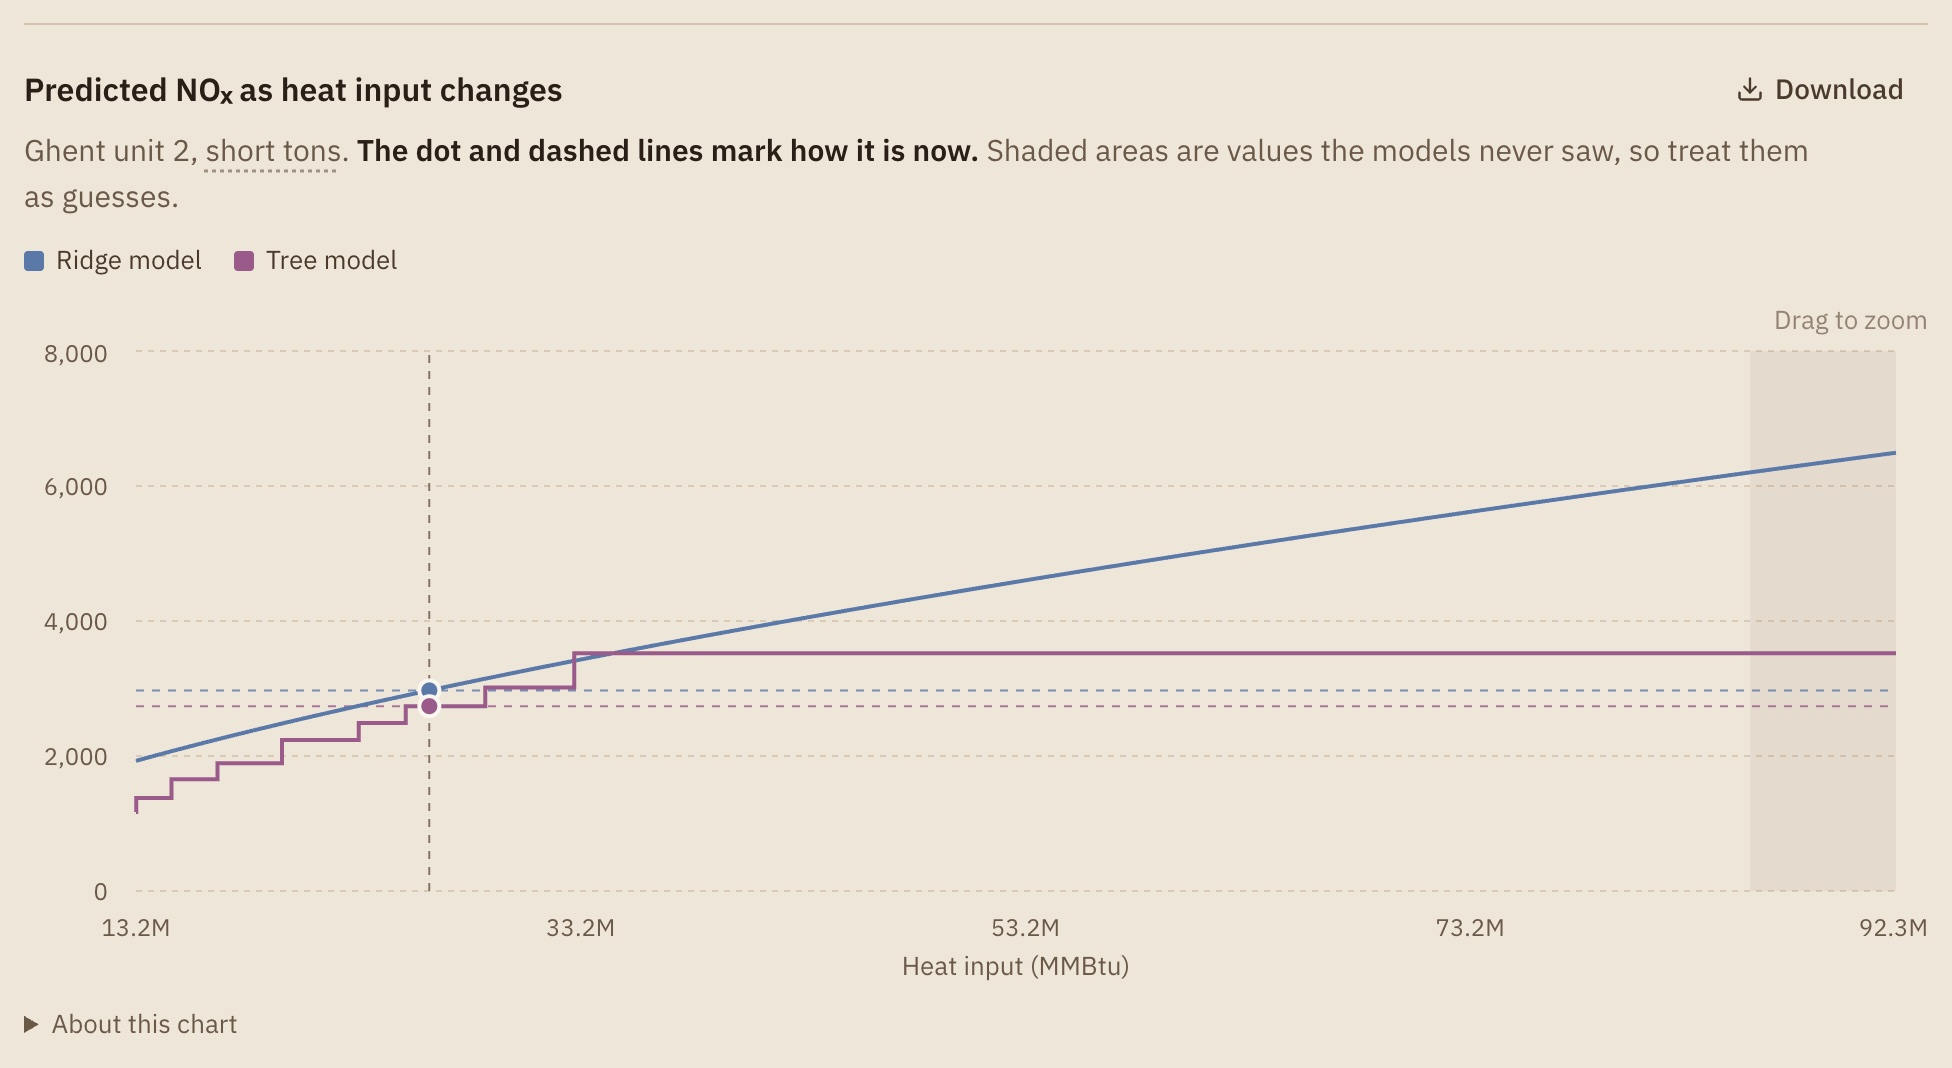
\includegraphics[width=\linewidth]{p2-sensitivity.jpg}
  \caption{Sensitivity of the Ridge and tree \NOx{} predictions to heat input for Ghent unit~2,
  2024, from $-50\,\%$ to $+250\,\%$. Shaded: outside the training data.}
  \label{fig:sensitivity}
\end{figure}

\paragraph{Sensitivity to a category.} Varying the primary fuel of the same unit
(Figure~\ref{fig:category}) shows the two models' structure directly. Ridge gives every fuel its
own coefficient: as reported (coal) it predicts 2{,}972 tons, as coal refuse 2{,}346 ($-21\,\%$),
as pipeline gas 928 ($-69\,\%$), and as process gas 537 ($-82\,\%$). The tree predicts 2{,}738
tons for every fuel, every unit type, and with or without SCR: its feature importances give heat
input 65\,\% and last year's \NOx{} rate 26\,\% of its error reduction, and SCR none, so no split
on this unit's path tests the fuel or the controls. The page's reading says so (``The tree barely
responds'').

\begin{figure}[!htbp]
  \centering
  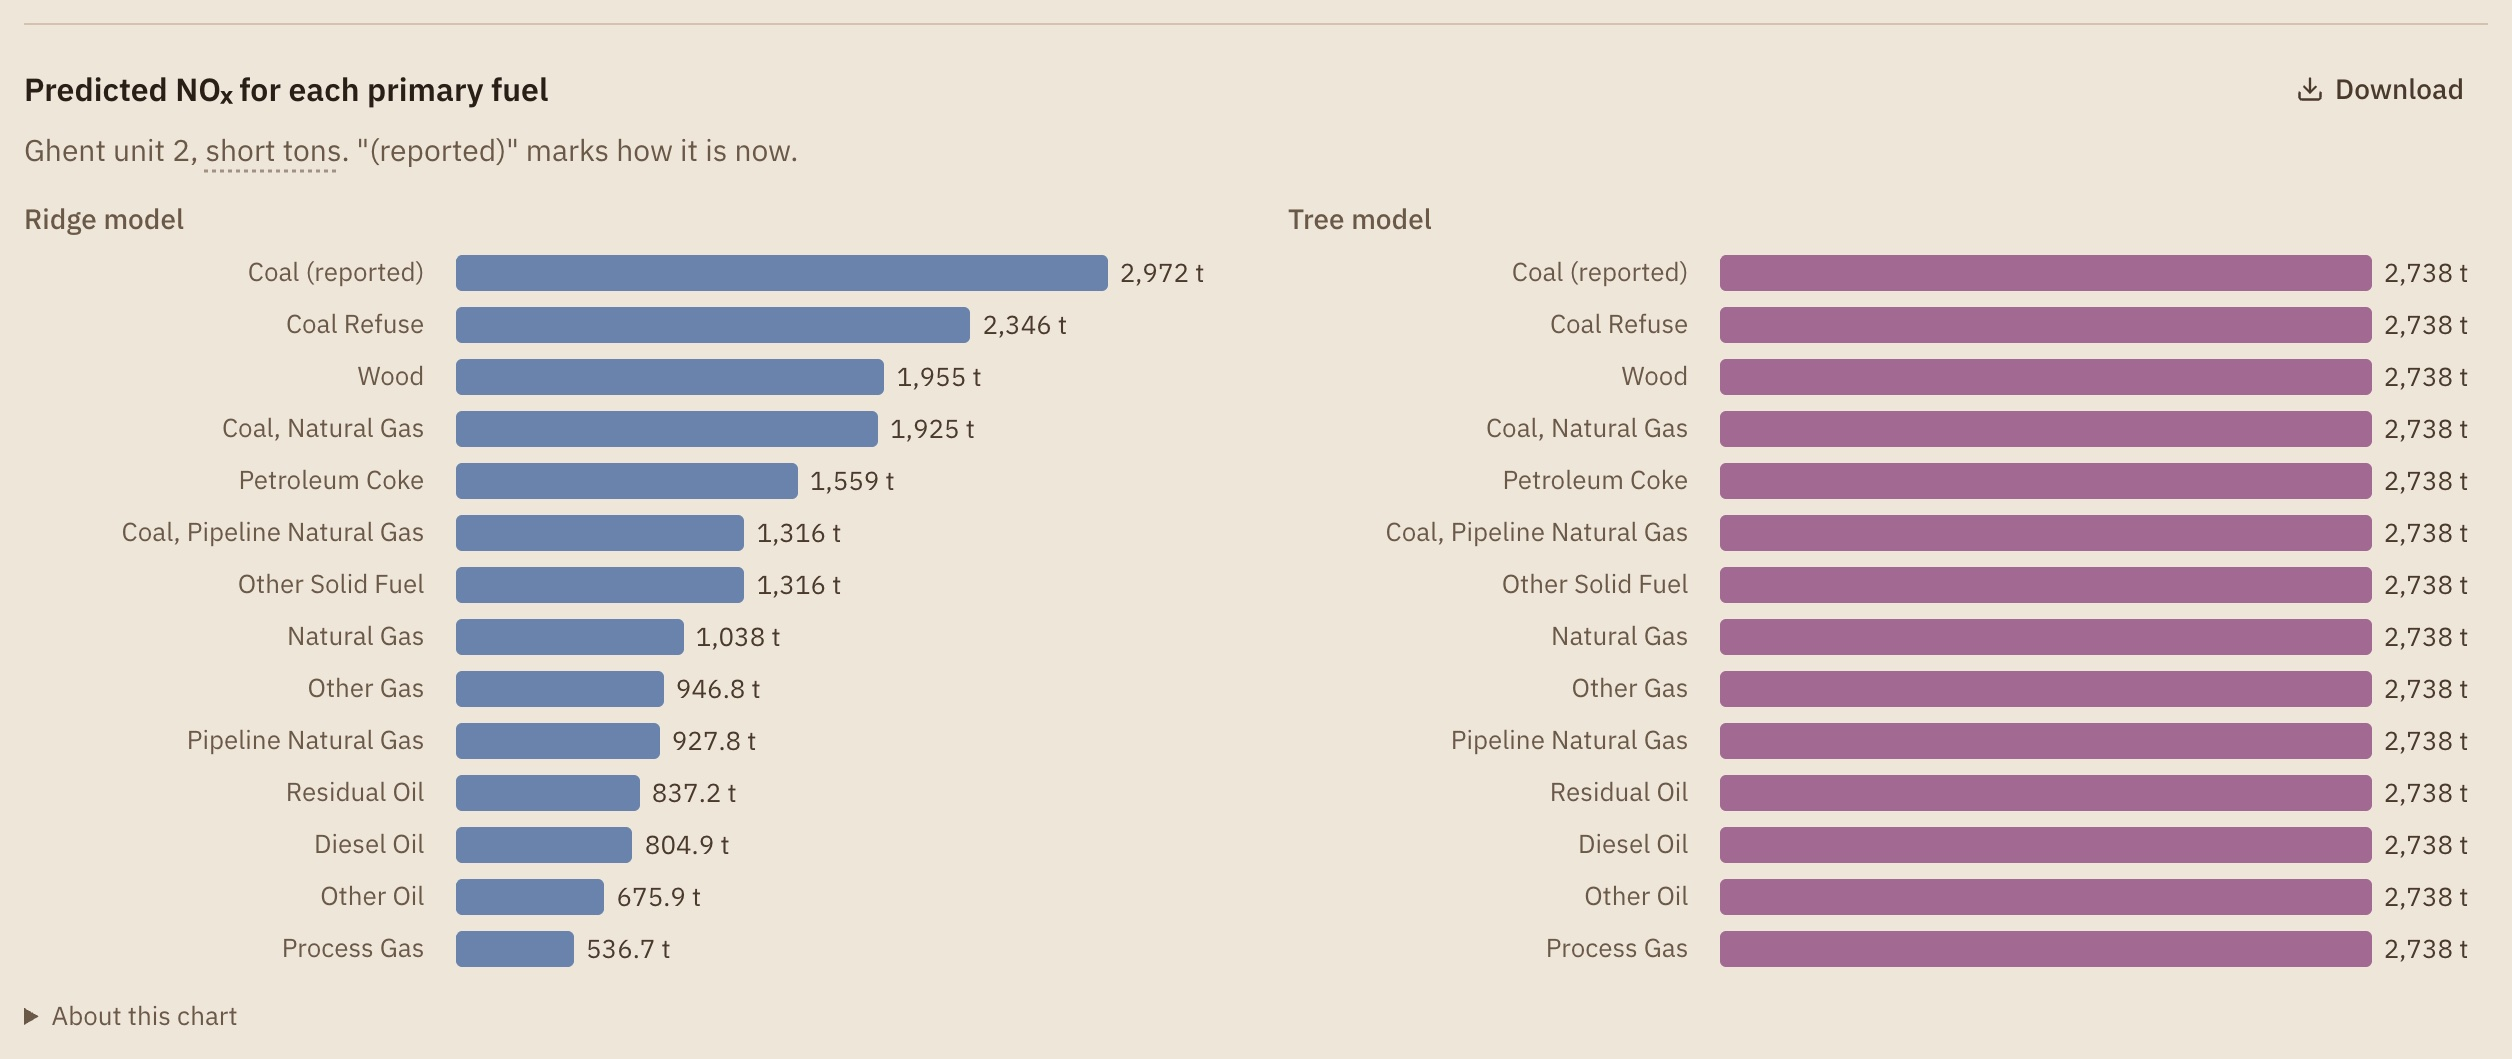
\includegraphics[width=\linewidth]{p2-category.jpg}
  \caption{Sensitivity to the primary fuel for Ghent unit~2, 2024: one bar per fuel seen in
  training, the unit's own fuel marked ``reported''.}
  \label{fig:category}
\end{figure}

\paragraph{Scenarios.} Figure~\ref{fig:scenarios} applies the named scenarios to the same unit.
The models move in the same direction when the unit runs 10\,\% more or less (Ridge $+6.2$ and
$-6.4\,\%$, tree $+10.1$ and $-9.1\,\%$) and when it makes the same power from 5\,\% less fuel
(Ridge $-3.2\,\%$, tree $-9.1\,\%$). Raising gross load by 10\,\% with heat input held fixed
changes neither prediction (Ridge $+0.03\,\%$, tree $0\,\%$): \NOx{} follows fuel burned, not
power sold. They disagree on controls and fuel. Ridge predicts that
adding SCR would cut \NOx{} by 59\,\%, the combined high-efficiency change by 60\,\%, and
switching to gas by 69\,\%; the tree predicts no change for SCR or gas, and for the combined
change only the 9\,\% of its lower fuel. The tree splits
mostly on heat input and the previous year's \NOx{} rate, which still describes the unit as it
was, so a changed control flag rarely changes its path. Ridge applies one average SCR
coefficient to every unit. Neither number is a causal estimate. When two reasonable models
disagree this much, the data do not determine the effect, and the page says so.

\begin{figure}[!htbp]
  \centering
  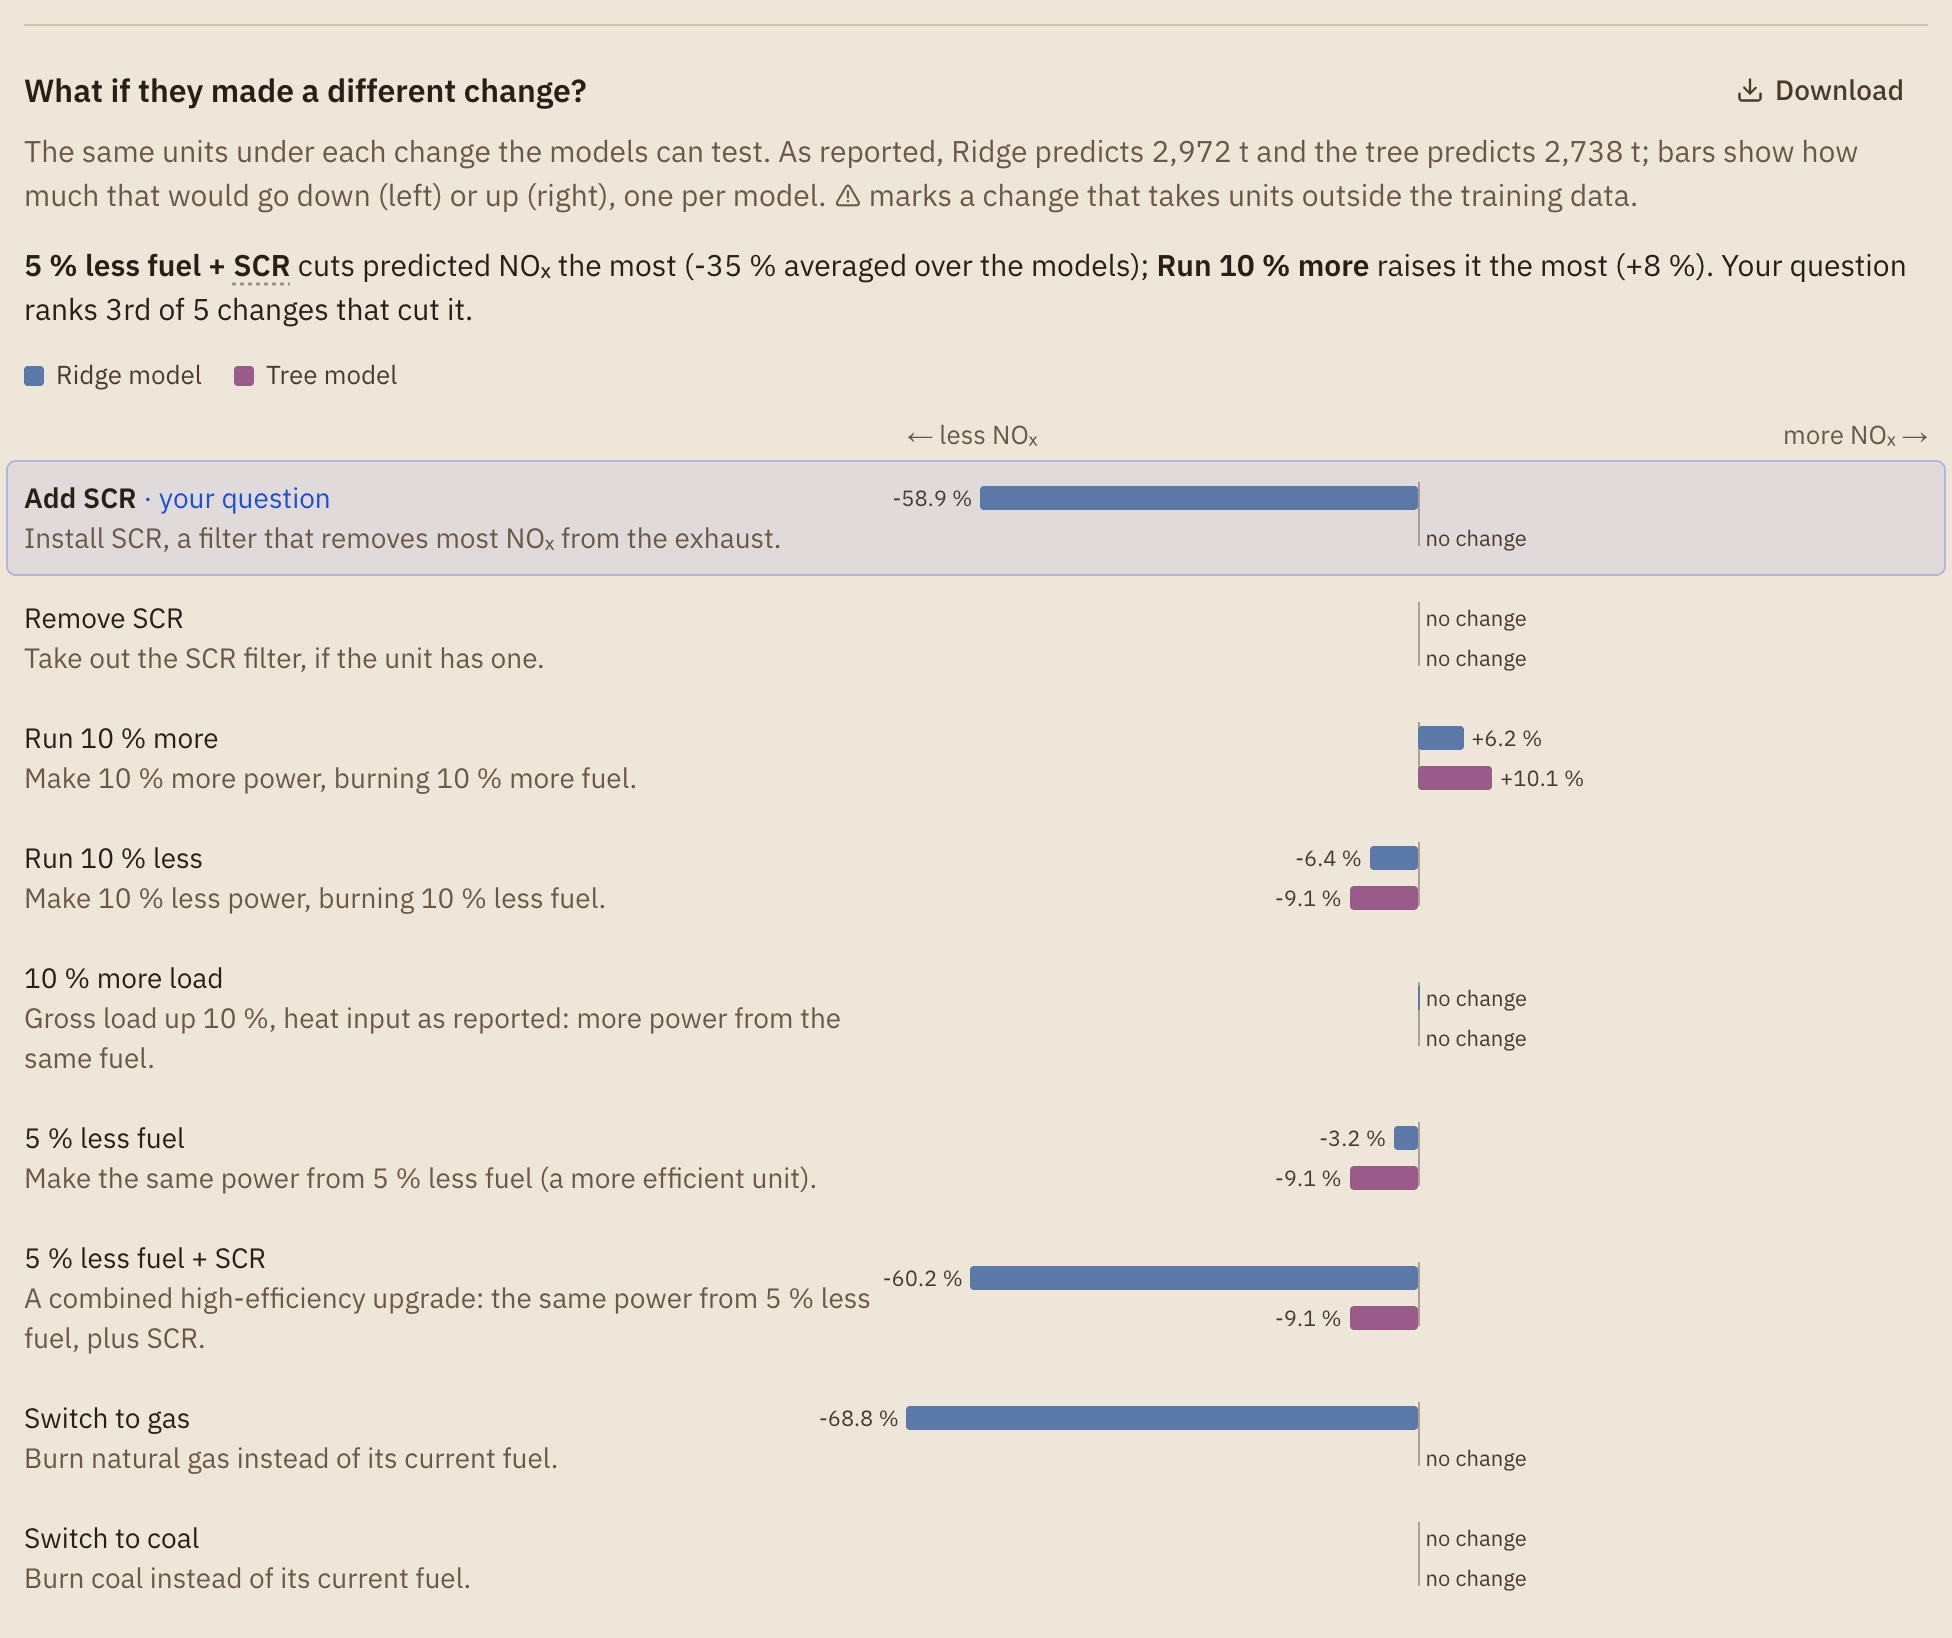
\includegraphics[width=\linewidth]{p2-scenarios.jpg}
  \caption{The nine named scenarios for Ghent unit~2, 2024, under Ridge and the decision tree;
  labels give the change from each model's baseline prediction.}
  \label{fig:scenarios}
\end{figure}

\paragraph{Scenario impacts.} Each TRACI category of \NOx{} is the predicted mass times a fixed
factor, so a scenario changes \NOx{}'s impacts by the same share as its \NOx{}, and the page says
so instead of repeating the table. Ridge's baseline of 2{,}972 tons is $6.68 \times 10^{7}$~kg
O\textsubscript{3}~eq of smog-formation potential, $1.89 \times 10^{6}$~kg \SOtwo{}~eq of
acidification, and 19{,}500~kg \PMtwofive{}~eq of particulate human health; adding SCR
($-58.9\,\%$, Figure~\ref{fig:whatif}) lowers these to $2.75 \times 10^{7}$, 776{,}000, and
8{,}007. These are \NOx{}'s share of each category only, since the models do not predict
\COtwo{} or \SOtwo{}, and they inherit the models' disagreement: under the tree, adding SCR
changes no impact at all.

\begin{figure}[!htbp]
  \centering
  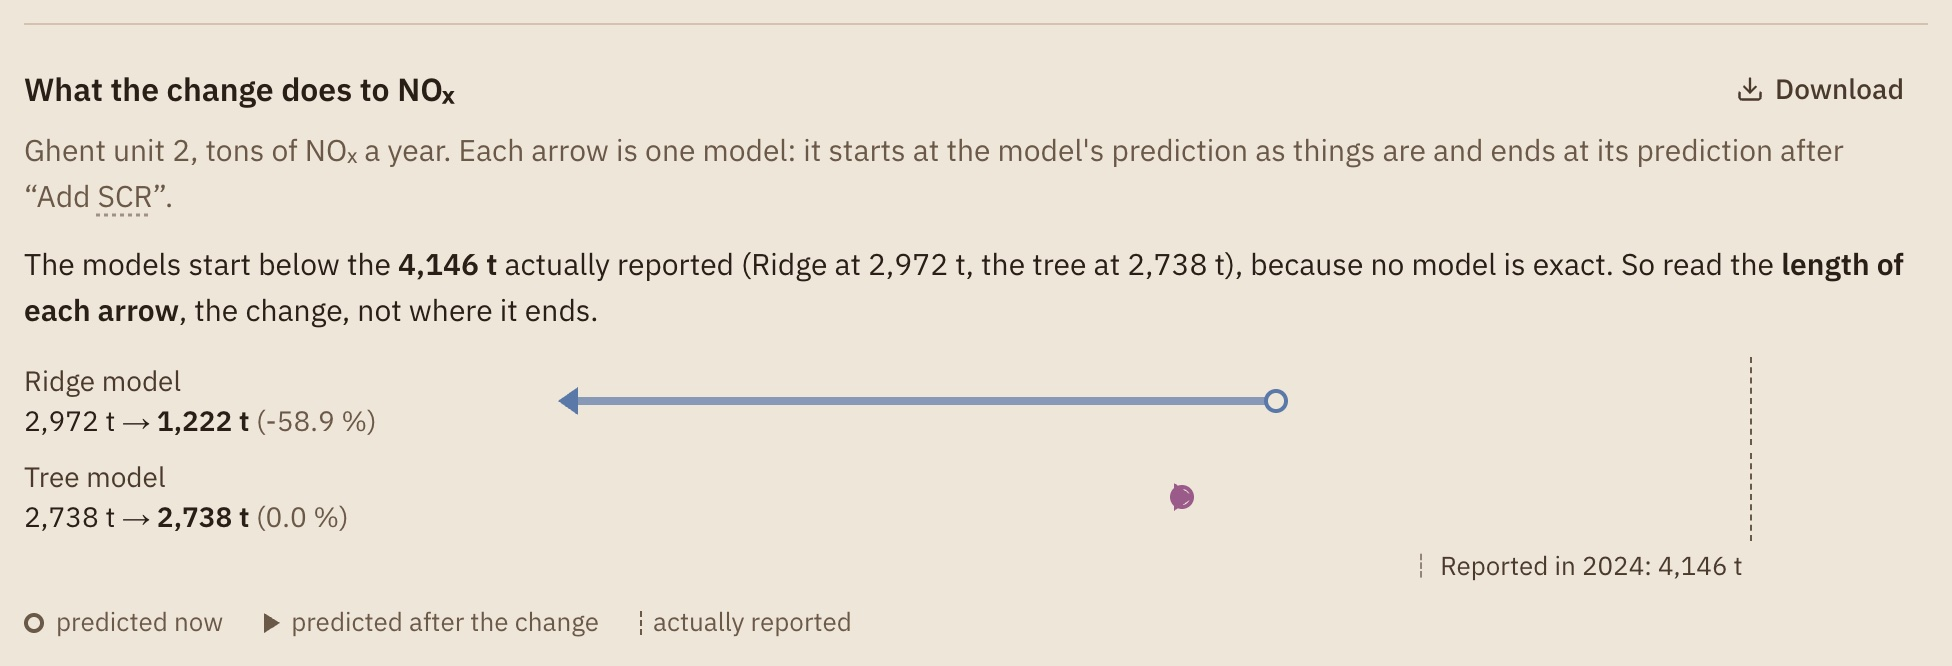
\includegraphics[width=\linewidth]{p2-whatif.jpg}
  \caption{What-if for Ghent unit~2, 2024, ``Add SCR'': each arrow runs from a model's prediction
  as reported to its prediction after the change; the dotted line is the \NOx{} actually
  reported.}
  \label{fig:whatif}
\end{figure}

% ------------------------------------------------------------------------
\section{Highlighted features}
\label{sec:features}

This section describes four implementation choices in more detail, with the code behind them.

\subsection{One variable catalogue for every analysis}
\label{sec:feat-variables}

Every measured value, derived rate, year-over-year change, and TRACI category is an object with
a key, unit, definition, aggregation rule, and a function that computes its value for one
unit-year (\code{buildVariables} in \code{src/lib/analysis.ts}). Statistics, charts,
comparisons, impacts, exports, and the Overview tab's variable list all read this one list, so each is written
once and works for all 29 variables. Rates are built by one helper that also stores the
numerator and denominator, which is what makes pooling possible (Listing~\ref{lst:ratio}).

\par\noindent\begin{minipage}{\linewidth}
\begin{lstlisting}[language=TypeScript, caption={Rates and pooling (\code{src/lib/analysis.ts}, abridged).}, label=lst:ratio]
/** A rate: null when either input is missing or the denominator is 0 (or negative). */
function ratio(base, num: Value, den: Value, scale = 1): Variable {
  return {
    ...base,
    aggregation: "ratio",
    ratio: { num, den, scale },
    value: (r) => {
      const n = num(r);
      const d = den(r);
      return n === null || d === null || d <= 0 ? null : (n / d) * scale;
    },
  };
}

/** A variable's value over a group, by its aggregation; null when no row defines it. */
export function aggregate(v: Variable, rows: readonly AnalysisRow[]) {
  let n = 0, sum = 0, num = 0, den = 0;
  for (const r of rows) {
    const x = v.value(r);
    if (x === null) continue;           // missing: skipped, never counted as 0
    n++;
    sum += x;
    if (v.ratio) {
      num += v.ratio.num(r)!;
      den += v.ratio.den(r)!;
    }
  }
  if (!n) return null;
  if (v.ratio) return den > 0 ? (num / den) * v.ratio.scale : null;
  return v.aggregation === "mean" ? sum / n : sum;
}
\end{lstlisting}
\end{minipage}

\subsection{TRACI impacts as ordinary variables}

Each TRACI category becomes two variables built from the rows of \code{traci\_factors}: the total
and the per-MWh rate. Because the factors come from the database, the formula shown in the
interface and written to export metadata is generated from the same rows used in the
calculation (Listing~\ref{lst:traci}).

\par\noindent\begin{minipage}{\linewidth}
\begin{lstlisting}[language=TypeScript, caption={Impact of one category for one unit-year (\code{impactVariables}, abridged).}, label=lst:traci]
const terms = factors.filter((f) => f.impactCategory === category);
const impact: Value = (r) => {
  let total = 0;
  for (const { p, factor } of parts) {   // one term per matched pollutant
    const tons = r[p.mass];
    if (tons === null) return null;     // a missing pollutant makes the category missing
    total += tons * SHORT_TON_KG * factor;   // SHORT_TON_KG = 907.18474
  }
  return total;
};
\end{lstlisting}
\end{minipage}

\subsection{Prediction without Python on the server}

\code{ml/train.py} implements its own preprocessing instead of scikit-learn's pipeline objects,
so that every step can be written to JSON. Missing numeric inputs are replaced by the training
median, three skewed inputs are log-transformed ($\log(1 + x)$), numeric inputs are standardized
with the training mean and standard deviation, fuel and unit type are one-hot encoded over
categories seen at least 30 times, and the control flags are passed through. Ridge stores its
coefficients and intercept; the tree stores its node arrays (children, split feature,
threshold, and leaf value). \code{src/lib/model.ts} repeats the same steps.

One detail mattered. scikit-learn compares tree features as 32-bit floats, so the TypeScript
version rounds each feature to single precision before comparing it with a threshold
(Listing~\ref{lst:tree}). Without this, a value that falls between a threshold's single- and
double-precision forms takes the wrong branch. A parity test replays 200 test-year unit-years
exported by the training script and requires each model's TypeScript prediction to equal
scikit-learn's within $10^{-6}$.

\par\noindent\begin{minipage}{\linewidth}
\begin{lstlisting}[language=TypeScript, caption={Tree inference (\code{predict} in \code{src/lib/model.ts}).}, label=lst:tree]
// scikit-learn trees compare float32 features against their thresholds.
const t = model.tree!;
let node = 0;
while (t.left[node] !== -1) {
  node =
    Math.fround(x[t.feature[node]!]!) <= t.threshold[node]!
      ? t.left[node]!
      : t.right[node]!;
}
return t.value[node]!;
\end{lstlisting}
\end{minipage}

\subsection{Exports that can be reproduced}
\label{sec:feat-export}

Exporting Kentucky, 2024 with Analyze's \emph{Download all} gives a ZIP with a CSV of 90 unit-years (one
column per variable) and the \code{metadata.json} shown, shortened, in
Listing~\ref{lst:meta}. The database snapshot and commit identify the data and code; the filters
and variable definitions say what was selected and how each column was computed; the factor
list makes every impact value checkable by hand.

\par\noindent\begin{minipage}{\linewidth}
\begin{lstlisting}[language={}, caption={\code{metadata.json} of an analytical-dataset export (shortened).}, label=lst:meta, numbers=none]
{
  "title": "Analytical dataset",
  "page": "Analyze",
  "exportedAt": "2026-11-20T01:35:05.412Z",
  "software": { "name": "epaData", "version": "0.1.0", "commit": "9236927" },
  "database": { "unitYears": 57414, "datasets": 153,
                "lastImport": "2026-10-11T04:38:52.000Z" },
  "filters": { "stateCode": "KY", "yearMin": "2024", "yearMax": "2024" },
  "unitYears": 90,
  "variables": [ { "key": "co2Intensity", "unit": "lb/MWh",
      "definition": "CO2 mass x 2,000 / gross load. Missing when either ...",
      "aggregation": "ratio" }, ... ],
  "traciFactors": [ { "traciVersion": "2.2", "pollutant": "nox",
      "substance": "NITROGEN OXIDES", "impactCategory": "Smog formation",
      "factor": 24.793589743589738, "factorUnit": "kg O3 eq" }, ... ],
  "missingValues": "Blank cells are missing: not reported, or undefined ..."
}
\end{lstlisting}
\end{minipage}

% ------------------------------------------------------------------------
\section{Testing and results}
\label{sec:testing}

\subsection{Approach}

Each calculation was tested against an independent reference: statistics against NumPy and
SciPy, TRACI results against hand calculation, TypeScript predictions against scikit-learn, and
counts against hand-written SQL. Every page and chart was then used in a headless browser
(Playwright with Chrome) on the development and production builds, at desktop and phone
widths, checking for console errors and reading each screenshot. Downloaded ZIP files were
unpacked and their CSV and metadata checked. On the hosted build we checked that Analyze and
Predict load with the same numbers and that Upload refuses to write.
\code{npm run validate} (formatting, linting, type checking, unit tests, and a production build)
passes.

\subsection{Unit tests}

\code{npm test} runs 116 TypeScript tests in fourteen files: 115 pass and one is skipped because it
needs a folder of raw CAMPD files that is not committed. Sixty-five tests in eight files cover
Phase~2:
\begin{itemize}
  \item \code{stats.test.ts} (5 tests): quantiles and standard deviation against NumPy; Pearson
        and Spearman correlation, Welch's $t$, Mann--Whitney $U$, the confidence interval,
        ANOVA, Kruskal--Wallis, and the $\chi^2$ tail against SciPy, to $10^{-9}$ for statistics
        and $10^{-6}$ for $p$-values; pairwise-complete correlation; constant inputs; and the
        heat map's correlation matrix, identical to the pair-by-pair values on columns with
        missing values and ties.
  \item \code{analysis.test.ts} (16 tests): each derived rate, and its missing value when an input
        is missing or a denominator is zero; capacity factor in leap and ordinary years;
        year-over-year changes with a missing or zero previous year; pooled rates as a ratio of
        sums; TRACI impacts against hand calculation, with categories kept apart and a missing
        pollutant affecting only its own categories; the factor extract (six factors, nitrogen
        oxides rather than nitrogen dioxide); the control classes; percentage formatting; the URL
        state (default year range, unknown fields, old tab links, a What-if question); and \code{findVariable}, which
        rejects an unknown variable key so that the server answers with an error (HTTP 400)
        instead of an empty result; the counts of each cause of missing values; and the TRACI
        impacts of a predicted \NOx{} mass, through the \NOx{} factors only.
  \item \code{model.test.ts} (13 tests): the parity test (all three models on 200 test
        unit-years, within $10^{-6}$); input derivation (unit age, control flags, and a previous
        rate that is missing when the previous heat input is zero); out-of-range detection; the
        direction of the response to heat input; readable feature names; and the What-if
        calculations: percentage change (undefined from zero); the sensitivity grid (minimum to
        maximum by the step, the baseline included once, a reversed range and a zero, negative,
        or empty step corrected and reported, the point limit); scenarios (scaled load and heat
        input, SCR and fuel set, never below zero, described in words) and the inputs each
        changes, named with their new and baseline values; group totals, as reported and under a
        scenario, equal to the sum of the units' predictions, and the group sensitivity and
        category curves; the tree's thresholds, between which its prediction is flat, and its
        path in words; and the signed and absolute error per fuel.
  \item \code{export-bundle.test.ts} (6 tests): a ZIP reads back as the CSV, \code{metadata.json},
        and PNG that went in; and the metadata of every kind of export (Analyze charts, the
        analytical dataset, and Predict) contains each of the six reproducibility items of
        \S7, while metadata missing any one of them is reported with that item's name.
  \item \code{takeaways.test.ts} (12 tests): the plain-language readings: a trend as a rise or
        fall, the largest group and its share, spread and outliers in words, a correlation's
        strength (skipping pairs that measure one quantity twice) and the two measures compared,
        a comparison, the model verdict against the baseline, the impact leaders, a What-if
        answer, a sensitivity from its minimum to its maximum, the chart readings, and the tree's
        path.
  \item \code{glossary.test.ts} (3 tests): table headers find their definition, and each term is
        marked once per block of text.
  \item \code{top-selection.test.ts} (5 tests): a Top~N selection (overall, per state, lowest
        first, or by rate) keeps the same facilities or unit-years on every page that uses it,
        including Analyze.
  \item \code{search-suggestions.test.ts} (5 tests): the filter values the search box suggests:
        states by name or postal code, values by word start or initials (``SCR''), a single year
        or a year range, applied values left out, and which suggestions are exact enough to lead
        the list.
\end{itemize}
\code{npm run test:py} runs ten pytest tests of the training pipeline: the three periods do not
overlap; no input is the target or derived from it; the input rules; the preprocessing
specification gives the same matrix after a round trip through JSON; the baseline is the group
median; MAPE ignores targets below one ton; persistence is the previous rate times heat input,
with the baseline as fallback and last year's tons in the ablation; the bootstrap intervals
contain the point estimates and detect a clearly better model; and the tree grid extends past
its earlier limit.

\subsection{Representative test cases}

Table~\ref{tab:cases} lists end-to-end cases. Each expected value comes from an independent
source, usually a hand-written SQL query against the committed database.

{\small
\begin{longtable}{@{}R{0.33\linewidth}R{0.34\linewidth}R{0.19\linewidth}c@{}}
\caption{Representative test cases.}\label{tab:cases}\\
\toprule
\textbf{Input} & \textbf{Expected (source)} & \textbf{Actual} & \textbf{Pass}\\
\midrule\endfirsthead
\toprule
\textbf{Input} & \textbf{Expected (source)} & \textbf{Actual} & \textbf{Pass}\\
\midrule\endhead
Analyze with default filters (2015--2025, operating time $>$ 0) & 45{,}441 unit-years, 1{,}560 facilities, 4{,}942 units (SQL) & Same & \checkmark\\
Same years without the operating-time filter & 46{,}988 unit-years; 1{,}547 more, all with 0 hours (SQL) & Same & \checkmark\\
Analyze: KY, 2023--2024 & 173 unit-years that ran; 177 with the operating-time filter removed (SQL) & 173; 177 & \checkmark\\
Program CSNOX, 2015--2025, operating-time filter removed & 24{,}676 whole-code matches; a substring match would give 25{,}882 (SQL) & 24{,}676 & \checkmark\\
\code{/analyze?tab=impacts} with no filter & Default range 2015--2025 applied & Same & \checkmark\\
\COtwo{} intensity with gross load 0 & Missing, not 0 (1{,}506 unit-years with \COtwo{} but no positive load) & Missing & \checkmark\\
Impacts, Ghent, 2024 & 12{,}744{,}620~kg \SOtwo{}~eq; 1.1006 per MWh (hand calculation) & Same & \checkmark\\
Compare 2024 \NOx{} rate, SCR vs no control & Pooled 0.037 and 0.159~lb/MMBtu over 1{,}547 and 479 unit-years (SQL) & Same & \checkmark\\
Models tab, test years & MAE 109.4, 58.5, 26.3~t; intervals as in Table~\ref{tab:models} (\code{metrics.json}) & Same & \checkmark\\
Persistence, 7{,}648 test unit-years with a previous rate & MAE 18.286~t (SQL) & 18.286~t & \checkmark\\
Analyze request with an unknown variable & HTTP 400, ``Unknown variable'' (tRPC error contract) & Same & \checkmark\\
TypeScript vs scikit-learn, 200 unit-years & Equal within $10^{-6}$ (parity fixture) & Equal & \checkmark\\
Ghent unit~2, 2024, heat input $+250\,\%$ & Outside training range (max 85.8 million MMBtu) & Warned, shaded & \checkmark\\
Sensitivity from $+80$ to $-20\,\%$, step 0 & Read low to high with a step of 5, both reported (\code{sensitivityGrid}) & Same & \checkmark\\
Scenarios, Ghent unit~2, 5\,\% less fuel + SCR & Ridge $-60.2\,\%$, tree $-9.1\,\%$ (direct model call) & Same & \checkmark\\
Scenarios, Ghent unit~2, add SCR & Ridge $-58.9\,\%$, tree $0.0\,\%$ (direct model call) & Same & \checkmark\\
Export dataset, KY, 2024 & 90 rows; metadata with filters, 29 variables, 6 factors; no \S7 item missing & Same & \checkmark\\
Upload or retrieve on the hosted build & Refused with a ``run locally'' notice & Refused & \checkmark\\
\bottomrule
\end{longtable}}

\subsection{Performance}
\label{sec:perf}

Table~\ref{tab:perf} gives server-side times on an Apple-silicon laptop (Node.js~26) over the
default 2015--2025 selection of 45{,}441 unit-years, as the median of three runs (re-measured on
17~November). They exclude the
network and chart drawing.

\begin{table}[H]
\centering\small
\caption{Measured computation times for the 2015--2025 selection.}
\label{tab:perf}
\begin{tabularx}{\linewidth}{@{}Lr@{}}
\toprule
\textbf{Operation} & \textbf{Time}\\
\midrule
Load the selection (first request, SQL query and join) & 0.6\,s\\
Load the same selection again (cache) & $<$\,1\,ms\\
Overview summary (missing counts of 29 variables, and their causes) & 217\,ms\\
Statistics of \NOx{} intensity by fuel class & 58\,ms\\
Trend of \COtwo{} by year and fuel class & 20\,ms\\
Comparison of two groups with all tests & 33\,ms\\
Correlation heat map, 11 variables, Pearson & 89\,ms\\
Correlation heat map, 11 variables, Spearman & 0.24\,s\\
Sensitivity curve, 61 tree predictions (browser code) & 0.2\,ms\\
Analytical-dataset export, 2015--2025 (ZIP, through the server) & 0.75\,s\\
\bottomrule
\end{tabularx}
\end{table}

Every operation in the table takes under a second, and a result already in \code{result\_cache}
is read in a few milliseconds instead. The Spearman heat map took 1.9~s until 11/12: it sorted
both variables again for each pair, because the pairwise-complete subset differs from pair to
pair, and computed both halves of the symmetric matrix. It now sorts each variable once, ranks a
pair's complete rows in one pass over that order, and computes each of the 55 pairs once, which
also shortens the Pearson map. A unit test checks that the matrix is identical to the pair-by-pair
calculation, and on the 2015--2025 selection both matrices are unchanged to the last digit.

\subsection{Defects found and corrected}

Testing found several defects, all corrected. The row cache stored a Drizzle query
instead of its result. Drizzle queries are lazy and run again on every \code{await}, so the
``cached'' selection was queried again for every view (1.5~s each); the loader now stores a
settled promise. The server export imported a module that defined a browser-side context, which
Next.js rejects in server code, so the dataset export failed; the context moved to the client
component that uses it. The year-range chip shared with the Explore page displayed
``2,015--2,025'' (a Phase~1 defect). A chart's loading placeholder and the Predict page's layout
at phone width were also fixed. The Python requirements had been pinned to versions that need
Python~3.11 or later, while the README documents Python~3.9; they are now minimum versions that
support both.

A final audit against the specification found five more. The emissions-program filter listed in
\S4.1 had never been built; it now matches a whole program code, because CAMPD stores lists such
as ``ARP, CSNOX, CSOSG2'' and a substring match would let ``CSNOX'' match ``CSNOXOS''. The
default 2015--2025 range applied only to a URL with no parameters at all, so a link to a tab
(\code{/analyze?tab=impacts}) analysed every year, including the partial 2026; it now applies
whenever the URL sets no filter. The row cache could miss an import for up to five minutes; its key
now includes the time of the latest import. A caption wrapped around a segmented control as an
HTML \code{label} passed a click on the caption to the first button, which changed the choice;
such captions are now plain groups. Sorting groups whose value was missing used an inconsistent
comparison.

\subsection{Known issues}
\label{sec:known}

\begin{itemize}
  \item On the Models tab, the predicted-against-actual chart and the error-by-fuel chart use
        an even sample of 3{,}000 test unit-years, so their numbers differ slightly from the full
        test set (Section~\ref{sec:results}); the metrics and \emph{All test predictions} use
        every unit-year.
  \item A link that sets any filter in the URL (for example a year) does not add the default
        operating-time filter, so it can select a few more unit-years than the same choice made
        on the page.
  \item Histograms, box plots, and scatter plots of very large selections draw a sample, as the
        chart states. Statistics are always computed on every value.
  \item Fuel and unit type are stored once per unit (Section~\ref{sec:limitations}).
\end{itemize}

\subsection{Assessment against the goals}
\label{sec:assessment}

Table~\ref{tab:objectives} assesses the nine goals of the Phase~2 specification.

\begin{table}[H]
\centering\small
\caption{Assessment of the Phase~2 goals.}
\label{tab:objectives}
\begin{tabularx}{\linewidth}{@{}>{\raggedright\arraybackslash}p{0.3\linewidth}p{1.5cm}L@{}}
\toprule
\textbf{Goal} & \textbf{Verdict} & \textbf{Evidence}\\
\midrule
G1 Descriptive statistics & Met & Distribution tab; checked against NumPy and SciPy.\\
G2 Comparisons & Met & Compare groups tab with tests and plain-language readings (Q2).\\
G3 Interactive visualization & Met & Seven chart types on Analyze and eight charts on Predict, all with tooltips and export, each tab with a reading.\\
G4 TRACI impacts & Met & Four categories TRACI~2.2 defines for these pollutants (Q3).\\
G5 Trends, relationships, unusual observations & Met & Q1, the correlation outlier, far-out fences.\\
G6 Prediction models & Met & Two models beat the baseline on held-out years, with intervals; neither beats persistence, and Q4 says why.\\
G7 Sensitivity and scenarios & Met & With range warnings.\\
G8 Saving and exporting & Met & Every result exports with metadata.\\
G9 Explaining methods and limitations & Met & Definitions, captions, and caveats in the interface; this report.\\
\bottomrule
\end{tabularx}
\end{table}

% ------------------------------------------------------------------------
\section{Discussion}
\label{sec:discussion}

\subsection{Effectiveness of techniques and tools}

Treating every derived indicator and TRACI category as an ordinary variable, with one
definition, unit, aggregation rule, and missing-value rule, was the most useful decision of the
phase. Statistics, charts, comparisons, impacts, and exports are each written once and work for
all 29 variables; adding a variable means adding its definition. Reusing the Phase~1 filters for
the analytical dataset meant the dataset builder came with every filter, its URL encoding, and
its tests already in place.

Offline training kept pandas and scikit-learn for fitting and tuning and TypeScript for
interactive use. The cost is that preprocessing is written twice, in \code{train.py} and
\code{model.ts}. The parity test makes this safe: it fails if one is changed without the other.

\subsection{Technical choices and alternatives}

\paragraph{Flask and pandas at request time.} The specification recommends computing analyses
with pandas behind Flask routes. Rewriting the Phase~1 application in Flask was not realistic,
and calling Python on each request (as Phase~1 does for uploads) would add a process start to
every chart and would not run on the hosted build. The statistics needed are few and well
defined, so implementing them in TypeScript and checking them against SciPy was the smaller and
safer option.

\paragraph{From Plotly.js to Recharts and D3.} The first version drew every chart with Plotly.js,
which the specification recommends and which provides every chart type it lists with tooltips,
zoom, and PNG export. Plotly charts, however, brought their own fonts, toolbar, and colors and did
not follow the application's light and dark themes without per-chart overrides, and the library
was by far the largest download of the site. Late in the phase we redrew every chart with
Recharts, whose charts are React components styled by the same design tokens as the rest of the
interface, and with D3 for the state map and heat map. The cost was rebuilding what Plotly gave
for free: drag-to-zoom, log axes with power-of-ten ticks, and PNG export (the chart's SVG is
drawn onto a canvas). Every chart kept its data export and metadata, and the export tests did
not change.

\paragraph{Ridge and a decision tree.} The two models were chosen to behave differently. Ridge
is smooth and gives each input one global effect, which makes sensitivity curves easy to read.
The tree captures interactions and thresholds and is much more accurate, but its response to one
input is a step function and it may ignore an input entirely. The scenario disagreement in
Section~\ref{sec:results} follows directly from this, and showing both models makes the
uncertainty visible. In hindsight, the persistence reference should have been computed first:
it sets the bar a model has to clear, and it showed that the inputs, not the choice between
these two models, limit the accuracy.

\subsection{Challenges and lessons learned}

The TRACI workbook needed care: it lists both nitrogen oxides and nitrogen dioxide with
different smog factors, and it has no eutrophication factor for these pollutants.
Reading the workbook itself, not a summary of it, avoided both errors. The parity test taught a
similar lesson: a TypeScript copy of a scikit-learn tree that looks correct still differs in
rare cases unless it reproduces the library's 32-bit comparison. Finally, the correlation
outlier showed that statistics over raw emissions data should be robust by default, since a
handful of unit-years with almost no generation can produce a near-perfect Pearson correlation
that describes nothing.

Missing values needed an explanation as well as a count. A table saying that 13.7\,\% of
unit-years lack \COtwo{} invites the conclusion that the data are poor. Counting the causes showed
that the gaps are rules of EPA reporting, not errors: 1{,}547 unit-years in 2015--2025 are units
that were listed but did not run, which is why Analyze leaves them out by default, and the
rest are units in \NOx{}-only programs, steam-only units, and first years without a previous year.
The data-quality section gives these causes, and in demonstrations it answers the question
before it is asked.

% ------------------------------------------------------------------------
\section{Limitations and recommended improvements}
\label{sec:limitations}

\subsection{Limitations}

\paragraph{Potential, not actual, impacts.} TRACI factors express potential contributions for
comparison. They ignore stack height, local population, weather, and background
concentrations, and they say nothing about actual illness or damage. Only the three pollutants
CAMPD reports are covered; particulate matter, mercury, and other emissions are not, and TRACI
2.2 has no eutrophication factor for these substances.

\paragraph{Missing pollutants remove categories.} A category is missing for a unit-year when one
of its pollutants is not reported. About 10.8\,\% of the 2015--2025 unit-years that ran lack
\SOtwo{} and 13.7\,\% lack \COtwo{} (mostly units in \NOx{}-only programs), so
their acidification and particulate results are missing, and group totals cover only the
unit-years that report every contributing pollutant. The Overview tab's data-quality section shows these counts.

\paragraph{Fuel and unit type are not stored per year.} As in Phase~1, fuel and unit type are
stored once per unit, so a unit that switched from coal to gas is treated as a gas unit in every
year, both in grouped statistics and as a model input.

\paragraph{Statistical independence.} Unit-years of the same unit are correlated, but the tests
treat them as independent, which overstates significance. A mixed model, or tests on one value
per unit, would be more rigorous.

\paragraph{Model responses are not causal.} Both models learn associations in observational data.
A scenario shows how a model responds when one input changes and everything else is fixed, which
may be physically impossible (for example more gross load with the same heat input). The
previous year's \NOx{} rate, the most useful history input, also encodes the unit's existing
controls, which weakens the models' response to a changed control and makes them slow to follow
a unit whose rate changes, as Ghent unit~2 shows. Range warnings check each input separately,
not the combination.

\paragraph{The models do not beat persistence.} Last year's \NOx{} rate times this year's heat
input predicts the test years more accurately than either model (Q4), and three reformulations
did not close the gap. The models are useful for exploring responses to inputs, not as the best
forecast of a unit's emissions.

\paragraph{Other limitations.} Analysis configurations are saved only as URLs. The year-over-year
variables compare consecutive years only, so a unit with a missing year has no change for the
following year.

\subsection{Recommended improvements}

The following changes would address the limitations above for anyone extending or maintaining
the system.
\begin{itemize}[itemsep=2pt]
  \item Store fuel and unit type per year, which would correct both the grouped statistics and the
        model inputs, and add the previous year's controls as inputs so that a model can see a
        control being installed.
  \item Use tests clustered by unit, or one value per unit, to give honest $p$-values.
  \item Try gradient-boosted trees with monotonic constraints, or separate models for coal and gas,
        for better accuracy and a more plausible response to controls.
  \item Replace the per-input range warning with a joint check, such as the distance to the
        nearest training unit-year.
\end{itemize}

% ------------------------------------------------------------------------
\section{Conclusions}
\label{sec:conclusions}

The application answers the four questions it was built around. The sector's \COtwo{} fell by
a fifth over 2015--2025 because generation moved from coal to gas, not because coal plants became
cleaner (Q1). Units with SCR emit \NOx{} at a much lower rate than uncontrolled units, although
the comparison mixes different fleets and is an association (Q2). TRACI totals and per-MWh results
rank states differently, and both views are needed to read them (Q3). The models beat the
baseline by a wide margin but not a simple persistence rule, so they are presented as tools for
exploring responses to load, fuel, and controls rather than as forecasts (Q4). Every result is
reproducible from its URL or its exported metadata, and the calculations are checked by 126
automated tests against NumPy, SciPy, scikit-learn, and hand-worked examples.

% ------------------------------------------------------------------------
\section{Individual contributions}
\label{sec:contributions}

Phase~2 kept the roles of Phase~1, a back-end lead and a front-end lead, with testing,
documentation, the report, and the presentation shared.

\paragraph{Raaj Banga (back-end lead).} The analytical data layer and the models: the variable
catalogue of derived indicators and year-over-year changes with their missing-value rules; the
statistics and hypothesis tests and their checks against SciPy; the TRACI~2.2 extract, the
\code{traci\_factors} and \code{models} tables, and the impact calculation; the analysis and
prediction procedures and the dataset export; the training pipeline in \code{ml/train.py}, the
TypeScript inference module, and the parity and pipeline tests; and the README,
\code{DATABASE\_BREAKDOWN.md}, and this report.

\paragraph{Arnav Bawankule (front-end lead).} The Phase~2 user interface: the Analyze page and
its Overview, Distribution, Relationships, Compare groups, and TRACI impacts tabs; the Predict
page and its Models and What-if tabs; the shared chart components (first on Plotly.js, then
redrawn with Recharts and D3), their theming, drag-to-zoom, and the export controls that save each
chart and table with its metadata; the filter chips, plain-language readings, and glossary; and
the presentation slides.

% ------------------------------------------------------------------------
\section{References and acknowledgments}
\label{sec:references}

\subsection{Data}

Emissions, operating, facility, and unit data are those of the Phase~1 database, from the EPA
Clean Air Markets Program Data~\cite{epa2026campd} (CAM API,
\url{https://www.epa.gov/power-sector/cam-api-portal}), a U.S.\ government work in the public
domain. TRACI~2.2 characterization factors are from the
EPA workbook \code{traci\_2\_2.xlsx}~\cite{epa2022traci22}, downloaded on 30~October 2026
(SHA-256 \code{80383dec\ldots 3725334}); only the six factors in Table~\ref{tab:factors} are
redistributed, in \code{data/traci/}.

\subsection{Reused code and assets}

Phase~2 builds on the Phase~1 code base and its libraries (Next.js~\cite{nextjs},
React~\cite{react}, SQLite~\cite{gaffney2022sqlite}). It adds Recharts~\cite{recharts} and
D3~\cite{bostock2011d3} for charts, topojson-client with the us-atlas state outlines (ISC
licence) for the map, fflate for ZIP files, and, in the offline pipeline,
pandas~\cite{mckinney2010pandas}, NumPy~\cite{harris2020numpy},
scikit-learn~\cite{pedregosa2011sklearn}, joblib, SciPy~\cite{virtanen2020scipy}, and pytest, all
used under their open-source licences. The chart components follow the patterns of the shadcn/ui
chart examples; no other external example code was copied.

\subsection{Generative AI disclosure}

In line with the course policy, we disclose that generative AI was used throughout this phase.
We used Anthropic's Claude, through the Claude Code tool, to help plan the phase, write and
review application, pipeline, and test code, investigate defects, capture screenshots, and draft
the README, the database documentation, and this report. The team defined the analytical
questions, the prediction target, and the design decisions, reviewed all generated code and
text, and accepted changes only after checking them with the type checker, linter, unit tests,
reference values from NumPy and SciPy, and manual use of the application. Every number in this
report was produced by running the application or the training pipeline against the committed
database. The team is responsible for the content of the code and of this report.

\renewcommand{\refname}{Bibliography}
\bibliographystyle{plain}
\bibliography{../shared/refs}

\vfill
\noindent\textit{We used AI to help with this project.}

\end{document}
